%
%---Beginning of Document---
%
\RequirePackage{lineno}
\documentclass[3p,times,twocolumn]{elsarticle}
\usepackage{lineno, color, listings, enumerate, amssymb, graphicx, float}
\usepackage{amsthm,amsmath}
% notice hyperref loaded last to avoid duplicate reference warnings
%\usepackage[font=normalsize,labelfont=bf]{caption}
\usepackage[pdfpagelabels]{hyperref}
\modulolinenumbers[5]
\usepackage[normalem]{ulem}
\usepackage[utf8]{inputenc}
\usepackage{soul}
\usepackage{dcolumn}% Align table columns on decimal pion\index{\footnote{}}t
\usepackage{bm}% bold math
\usepackage{hyperref}
\usepackage{epstopdf}
\usepackage{subcaption}
\usepackage{url}
\hyphenpenalty=1500
\exhyphenpenalty=1500

\def\etal{{\it et al.}}
\def\MaPMT{MaPMT }
\def\MaPMTs{MaPMTs }
\def\MAROC{MAROC3 }
\def\dT{$\Delta T$ }

%\documentclass{elsart}
%%\setcounter{footnote}{0}
%\setcounter{tocdepth}{5}
%\linenumbers

\begin{document}
\begin{frontmatter}

\title{CLAS12 Software Framework and Event Reconstruction}

\author[JLab]{V. Ziegler \corref{mycorrespondingauthor}}
\cortext[mycorrespondingauthor]{Corresponding author}
\ead{ziegler@jlab.org}
\author[JLab]{N. Baltzell}
\author[Saclay]{F. Boss\`u}
\author[JLab]{D.S. Carman}
\author[IPNO]{P. Chatagnon}
\author[INFN]{M. Contalbrigo}
\author[INFN]{R. De Vita}
\author[Saclay]{M. Defurne}
\author[JLab]{G. Gavalian}
\author[JLab]{Y. Gotra}
\author[JLab]{V. Gyurjyan}
\author[JLab]{N. Harrison}
\author[CNU]{D. Heddle}
\author[IPNO]{A. Hobart}
\author[UConn]{A. Kim}
\author[JLab]{N. Markov}
\author[JLab]{M.D. Mestayer}
\author[CNU]{W. Phelps}
\author[IPNO]{S. Niccolai}
\author[Glasgow]{D. Sokhan}
\author[JLab]{M. Ungaro}

\address[JLab]{Thomas Jefferson National Accelerator Facility, Newport News, VA 23606, USA}
\address[CNU]{Christopher Newport University, 1 Avenue of the Arts, Newport News, 23606 VA , USA}
\address[UConn]{University of Connecticut, Storrs, CT 06269, USA}
\address[INFN]{INFN, Sezione di Genova, 16146 Genova, Italy}
\address[Saclay]{CEA-Saclay, Univ. Paris-Sud, Universit\'e Paris-Saclay, Gif-sur-Yvettes, France}
\address[IPNO]{Institut de Physique Nucl\'eaire, CNRS-IN2P3, Univ. Paris-Sud, Universit\'e Paris-Saclay,
91406 Orsay Cedex, France}
\address[Glasgow]{University of Glasgow, Glasgow G12 8QQ, United Kingdom}
%\thanks[corresponding]{Corresponding author. Address: 12000 Jefferson Ave., Newport News, VA;

%\date{\today}

%\maketitle

\begin{abstract}
  We describe offline event reconstruction for the CEBAF Large Acceptance Spectrometer at 12~GeV (CLAS12),
  including an overview of the offline reconstruction framework and software tools, a description of the algorithms
  developed for the individual detector subsystems, and the overall approach for charged and neutral particle
  identification. We also present the scheme for data processing and the code management procedures.
\end{abstract}

\begin{keyword}
CLAS12, event reconstruction, PACS:29.40.Mc
\end{keyword}

\end{frontmatter}

%\tableofcontents

%\vfil
%\eject

\section{Introduction}
\label{introduction}

The physics program for CLAS12 in Jefferson Lab's Hall B requires the use of electron beams of various energies and currents that impinge
upon on targets ranging from liquid hydrogen to lead. A significant part of the physics program includes running with polarized targets that 
require a rastered beam on the target. In order to extract experimental observables, accurate measurements of the beam charge and 
polarization are required. Also, for safe and efficient operation of a large, open acceptance spectrometer, proper shielding and a stable beam 
with a small lateral size and minimal beam halo are needed. 

The Hall-B beamline is designed to satisfy experimental requirements and provide necessary controls and monitoring 
of the electron beam properties for safe and efficient operation of CLAS12. The key set of parameters required by experiments with CLAS12 
is listed in Table \ref{tab:beam_par}. The main challenges for the beamline setup are the open acceptance of CLAS12 and the close proximity 
of various sensitive detectors to the target and beam. Such challenges were successfully overcome in Hall B in the past for CLAS \cite{CLAS} 
experiments and the Heavy Photon Search (HPS) experiment \cite{HPS}.

 \begin{table}[htb]
 \centering
 \begin{tabular}{|c|c|c|}
\hline
Parameter & Requirement &Unit \\ \hline 
$E$ &  $\le 11$& GeV \\ \hline
$\delta p/p$ & $< 10^{-4}$ & \\ \hline 
Current & $<~500$ & nA \\ \hline
Current instability & $\sim 10$ &\% \\ \hline 
$\sigma_x $, $\sigma_y$&$< 300$& $\mu$m \\ \hline 
Position stability &$< 200$ &$\mu$m \\ \hline
Divergence& $< 100$& $\mu$rad \\ \hline 
Beam halo ($> 5\sigma$) &$< 10^{-4}$& \\ \hline
Beam polarization &$> 0.85$& \\ \hline
\end{tabular}
\caption{Nominal required Hall B beam parameters.} 
\label{tab:beam_par}
\end{table}

A few key modifications to the beamline \cite{HPSBeamline} used during the lower-energy run of the HPS experiment have been introduced 
in order to establish high-quality physics beams in Hall B and run CLAS12 at the design luminosity of $10^{35}$ cm$^{-2}$s$^{-1}$.  
Additions to the beamline for high-energy running of CLAS12 include a new intermediate beam dump upstream of the hall, a cryogenic 
target system, shielding downstream of the target to protect CLAS12 detectors from electromagnetic backgrounds, and the M{\o}ller 
polarimeter for beam polarization measurements.   

%\begin{figure*}[t]
%\begin{center}
%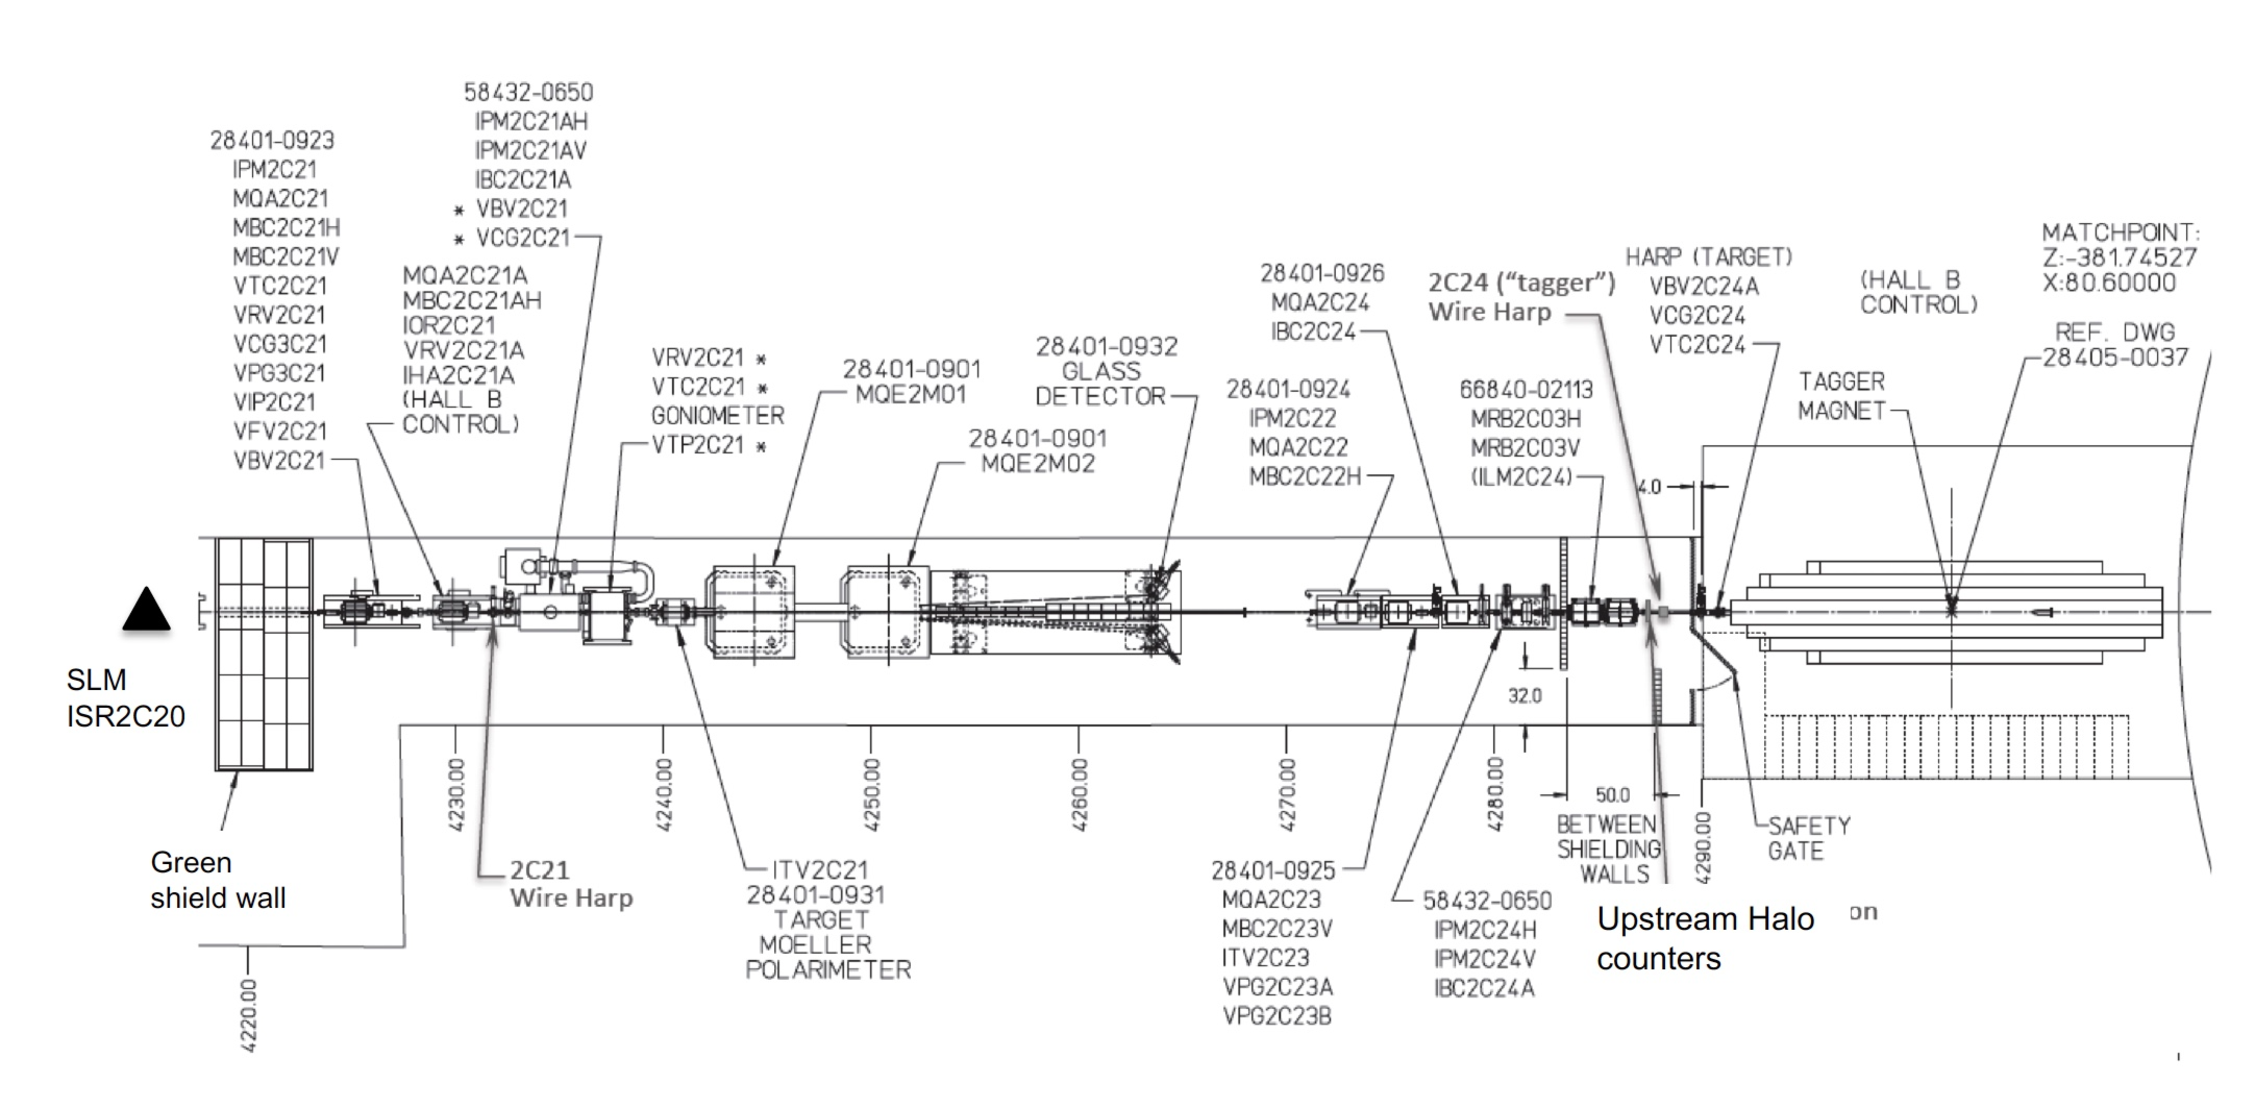
\includegraphics[width=1.\textwidth]{upstream_tunnel.pdf}
%\caption{Overhead view of the 2C beamline in the tunnel upstream of Hall B. {\color{red} Not the final figure.}}
%\label{fig:upstream}
%\end{center}
%\end{figure*}

 
This paper will discuss the design of the Hall-B beamline for CLAS12, and its performance during the 2018 experimental run. It will review the 
beamline instrumentation used to measure and monitor beam parameters and to protect CLAS12 detectors against errant beam motion. As will 
be demonstrated, excellent quality and stability of the CEBAF beams, coupled with the Hall-B beamline protection systems, allowed running the 
CLAS12 detector at the design luminosity.



%%%%%%%%%%%%%%%%%%%%%%%%%%%%%%%%%%%%%%%%%%%%%%%%%%%%%%%%%%
\begin{figure*}
\centering
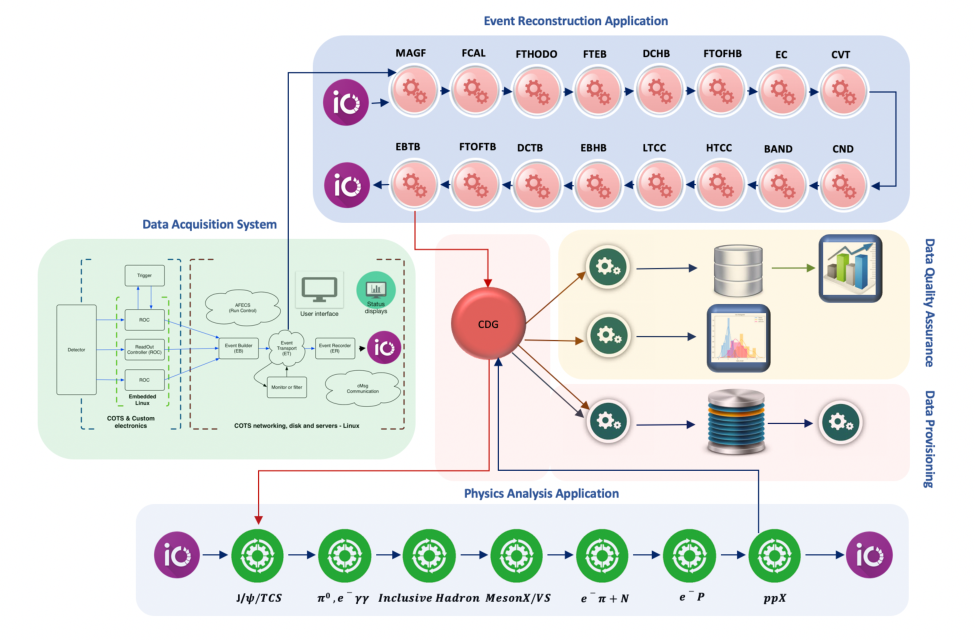
\includegraphics[width=0.8\textwidth]{pics/clara-overview.pdf}
\caption{Overview of the CLAS12 CLARA data processing framework.  Individual detector subsystem reconstruction applications can be linked to. form the full event reconstruction chain, including  data processing, data quality monitoring, and physics analysis applications.}
\label{fig:clara-overview}
\end{figure*}
%%%%%%%%%%%%%%%%%%%%%%%%%%%%%%%%%%%%%%%%%%%%%%%%%%%%%%%%%%%

\section{Software Framework and Tools}\label{sec:framework}

%Experimental physics data analysis in a collaborative environment has historically involved a computing model based on self-contained, monolithic software applications running in batch-processing mode. This model, if not organized properly, can result in inefficiencies in terms of deployment, maintenance, response to program errors, update propagation, scalability and fault-tolerance. Over time, experimental configurations have become more diverse and compute capacity has expanded at a rate consistent with Moore's Law. As a consequence, compute applications have become much more complex, with significant interaction between diverse program components.  This can lead to computing systems so complex and intertwined that the programs become difficult to maintain and extend. Modifying a feature in one class often involves changes in several other classes, thereby increasing the needed development time and effort. What starts small and simple, inevitably grows into a complicated scheme of interconnected algorithms. At some point, to prevent further growth in complexity, the software has to be shielded from contributors, preventing essential software evolution and optimization. The only way to bypass this highly guarded system is software fragmentation, making the physics data processing validation process quite arduous.

Nuclear and particle physics data processing applications must guarantee a long lifetime, larger than the multi-year duration of the corresponding experiment. The ability to upgrade and adapt technologies is therefore essential, so these applications should be organized in a way that easily permits upgrade of aged software components and inclusion of new ones, without need for major redesign or structural changes.  Support for software evolution and diversification (e.g. compatibility with heterogeneous hardware structures, such as FPGAs and GPGPUs) is important to accommodate more efficient and robust data processing applications in the future.


Following these principles, CLAS12 reconstruction and analysis relies on a data-stream processing framework called CLARA \cite{clara-2011,clara-service,framework,clara-2016}, which provides a service-oriented architecture in which to build the relevant software applications.  Such applications are composed of interlocking building blocks called micro-services, which are linked together by data-stream pipes.  The technology (e.g. a high-level programming language, or hardware deployment details) as well as the algorithmic solutions used to process data (see Fig.~\ref{fig:clara-overview},) are encapsulated.
The scope of a specific software application implemented in CLARA is determined by the micro-services that are included and by the order of their execution.

A micro-service has input data, processes it, and produces output data, where that I/O is organized in ``banks'' whose structure is configured by the specific service developer.  A micro-service reacts on a streaming data quantum in its input, processes it, and passes processed data quanta to the next micro-service in the data-flow path.  As a result, the CLAS12 data processing application is versatile and flexible, since the application building blocks can be improved individually and replaced with no need of structure changes in the framework. The CLAS12 micro-services are extensions of an abstract reconstruction engine, which includes common components such as initialization and events processing methods. This approach reduces and simplifies the development of an individual micro-service and enforces a common structure. 

%\sout{The CLAS12 data processing applications execute according to the rules of data-flow instead of a more traditional programming approach, where sequential series of instructions (lines of code) are written to perform a required algorithm. The flow of data between micro-services in the application determines the execution order of micro-services within the application. These features make the data paths between application building blocks to be the application designer’s main focus.}

The CLARA data-stream pipe is a data bus based on the xMsg messaging system that supports various protocols such as MPI, pub-sub, p2p, inproc, and shared memory. The CLARA orchestrator, i.e. the process level workflow management systems, controls the overall process execution. 

The framework enables execution of software applications in multi-threaded mode. This is implemented via event parallelization for the CLAS12 reconstruction. Figure~\ref{fig:scaling} shows the results of a scaling test on an Intel Xeon node (E5-2697A v4 @ 2.6GHz). Comparison with Amdhal's law indicates 99.5\% parallel efficiency over the 32 physical core of the machine.
{\color{red} SHOULD ADD MORE ON EVENT PARALLELIZATION AND MULTI-HW SUPPORT.}
\begin{figure}
\centering
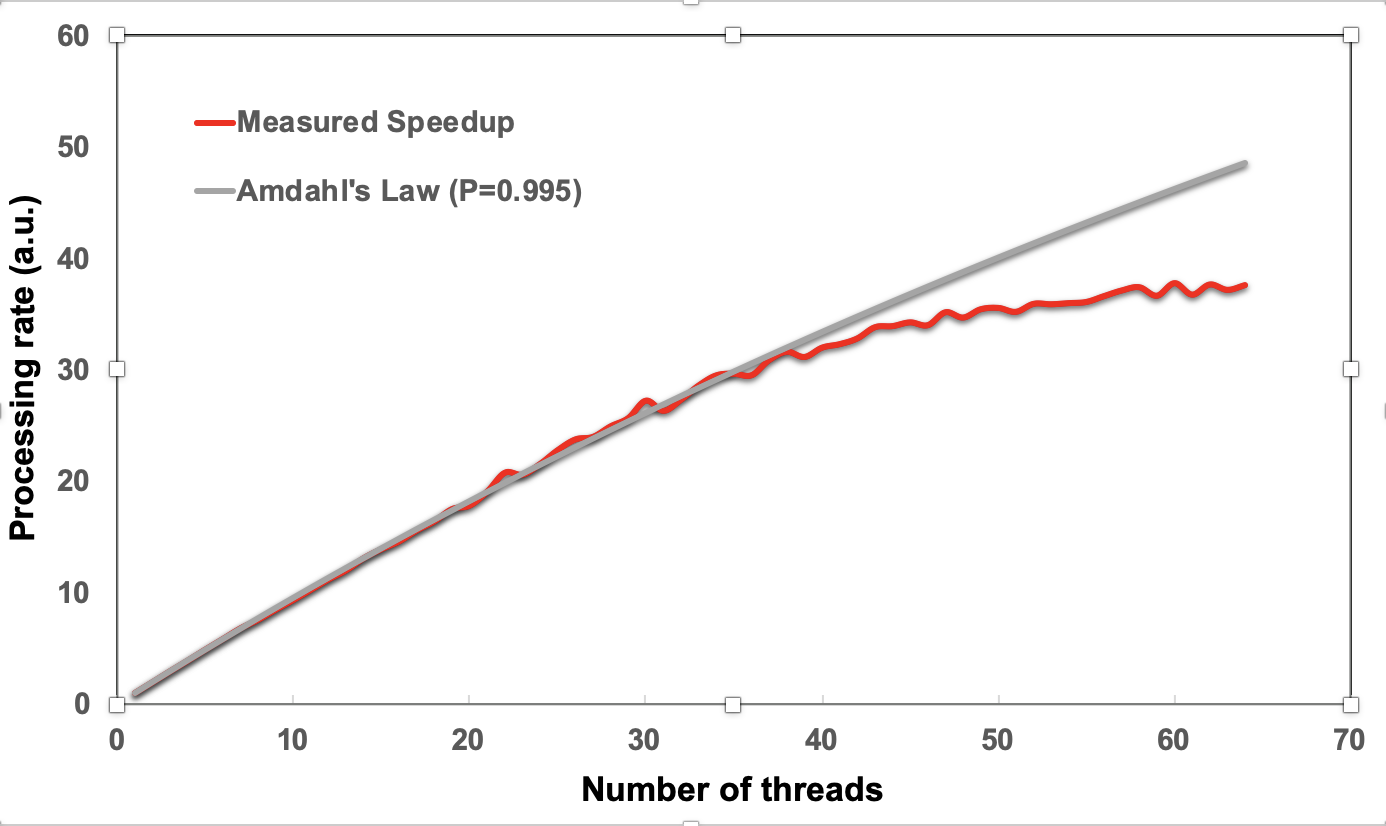
\includegraphics[width=0.48\textwidth]{pics/scaling.png}
\caption{Scaling of the CLAS12 event reconstruction application as implemented in the CLARA framework. Tests were conducted on a Intel Xeon node (E5-2697A v4 @ 2.6GHz). Comparison with Amdhal's law indicates 99.5\% parallel efficiency over the 32 physical core of the machine.}
\label{fig:scaling}
\end{figure}

\subsection{Common Tools}
\label{common-tools}

The offline software of the CLAS12 project aims at providing tools that allow design, simulation, and data analysis to proceed in an efficient, repeatable, and understandable way. Most  software engineering details are hidden from users, allowing them to concentrate on the algorithms and physics.  To facilitate code development for the detector subsystems of CLAS12, the software was designed to provide libraries that are commonly used by all the reconstruction packages.  These libraries, referred to as ``common tools'', facilitate avoiding replication and aid in software maintainability.

The common tools consist of various packages, each having a specific purpose and functionality. Below we discuss
the main packages used in the reconstruction software.

\subsubsection{Geometry}

Due to the complexity of the geometry of CLAS12 detector subsystems, an interface was developed to provide classes and software tools that are used to describe the geometry of all subsystem in an unified way.  A library of primitives provides geometrical objects needed to represent all detector subsystems (these include lines, planes and various shapes as for example cubes, trapezoids, etc.) and provide the necessary transformations to accommodate misalignments and distortions.  Furthermore, geometry tools provide methods to track particles through volumes for evaluation of track trajectories, such as line to surface intersections, ray tracing through objects, and distance of closest approach to a line or surface.

The CLAS12 geometry library is initialized from a database containing key geometry parameters and their variations for every detector.  This maximizes flexibility, supports time-dependent experiment geometry conditions, and ensures consistency between the simulation, reconstruction, and event visualization packages in Section \ref{sec:ced} \cite{sim-nim}. 

To facilitate development of new detector geometries, visualization capalities are included in the geometry library. Fig.~\ref{fig:detectorview} shows a view of part of the CLAS12 spectrometer using this functionality.


\subsubsection{Databases}

The Calibration Constant Data Base (CCDB) software package was developed at Jefferson Lab for the GlueX experiment
in HallD~\cite{gluex}.  CCDB provides the functionality for storing and accessing structured tables in MySQL-based and SQLite portable databases.
The CLAS12 reconstruction packages use the CCDB application programming interface to create and access
tables that contain detector geometry and calibration constants, as well as maps used for decoding raw data.

The CCDB package creates
tables that link constants to specific runs (using timestamps) and store different variations of constants depending on run
conditions. CLAS12 software tools employ an Application Programming Interface (API) that parses database tables and creates
structured maps of constants stored in  memory by detector sector, layer and component. This allows fast retrieving of the
constants.

The CLAS12 database access tools have been developed to avoid bottlenecks that might result from multiple multi-threaded
services accessing the database to retrieve constants.  An interface has been designed to fetch the constants
on demand and cache them for further requests. In this approach each service will request the
constants it requires on one thread and each subsequent request by a new thread will be provided by the cached values.

\subsubsection{Plotting and Analysis Tools}

For ease of integration with the reconstruction software tools and packages, the plotting tools used for data
calibration, monitoring and analysis was developed in the JAVA programming language.

The plotting software, called {\it groot}, developed at Jefferson Lab for CLAS12 is tailored to have a programming
interface similar to the CERN data analysis package, ROOT, and provides the the necessary functionalities for histogram and graphs creation, filling and manipulation as well as for fitting using the JAVA-based MINUIT library available from the JHEP repositories. This has been the base for the development of detector monitoring and calibration suites (see Sec.~\ref{sec:calibration}.

These same tools can be used for analysis purposes. In addition, the analysis package contains classes for four-vector manipulations and physics quantities extractions and
analysis methods (e.g. $Q^2, W$, boosts, etc.).

\begin{figure}
\centering
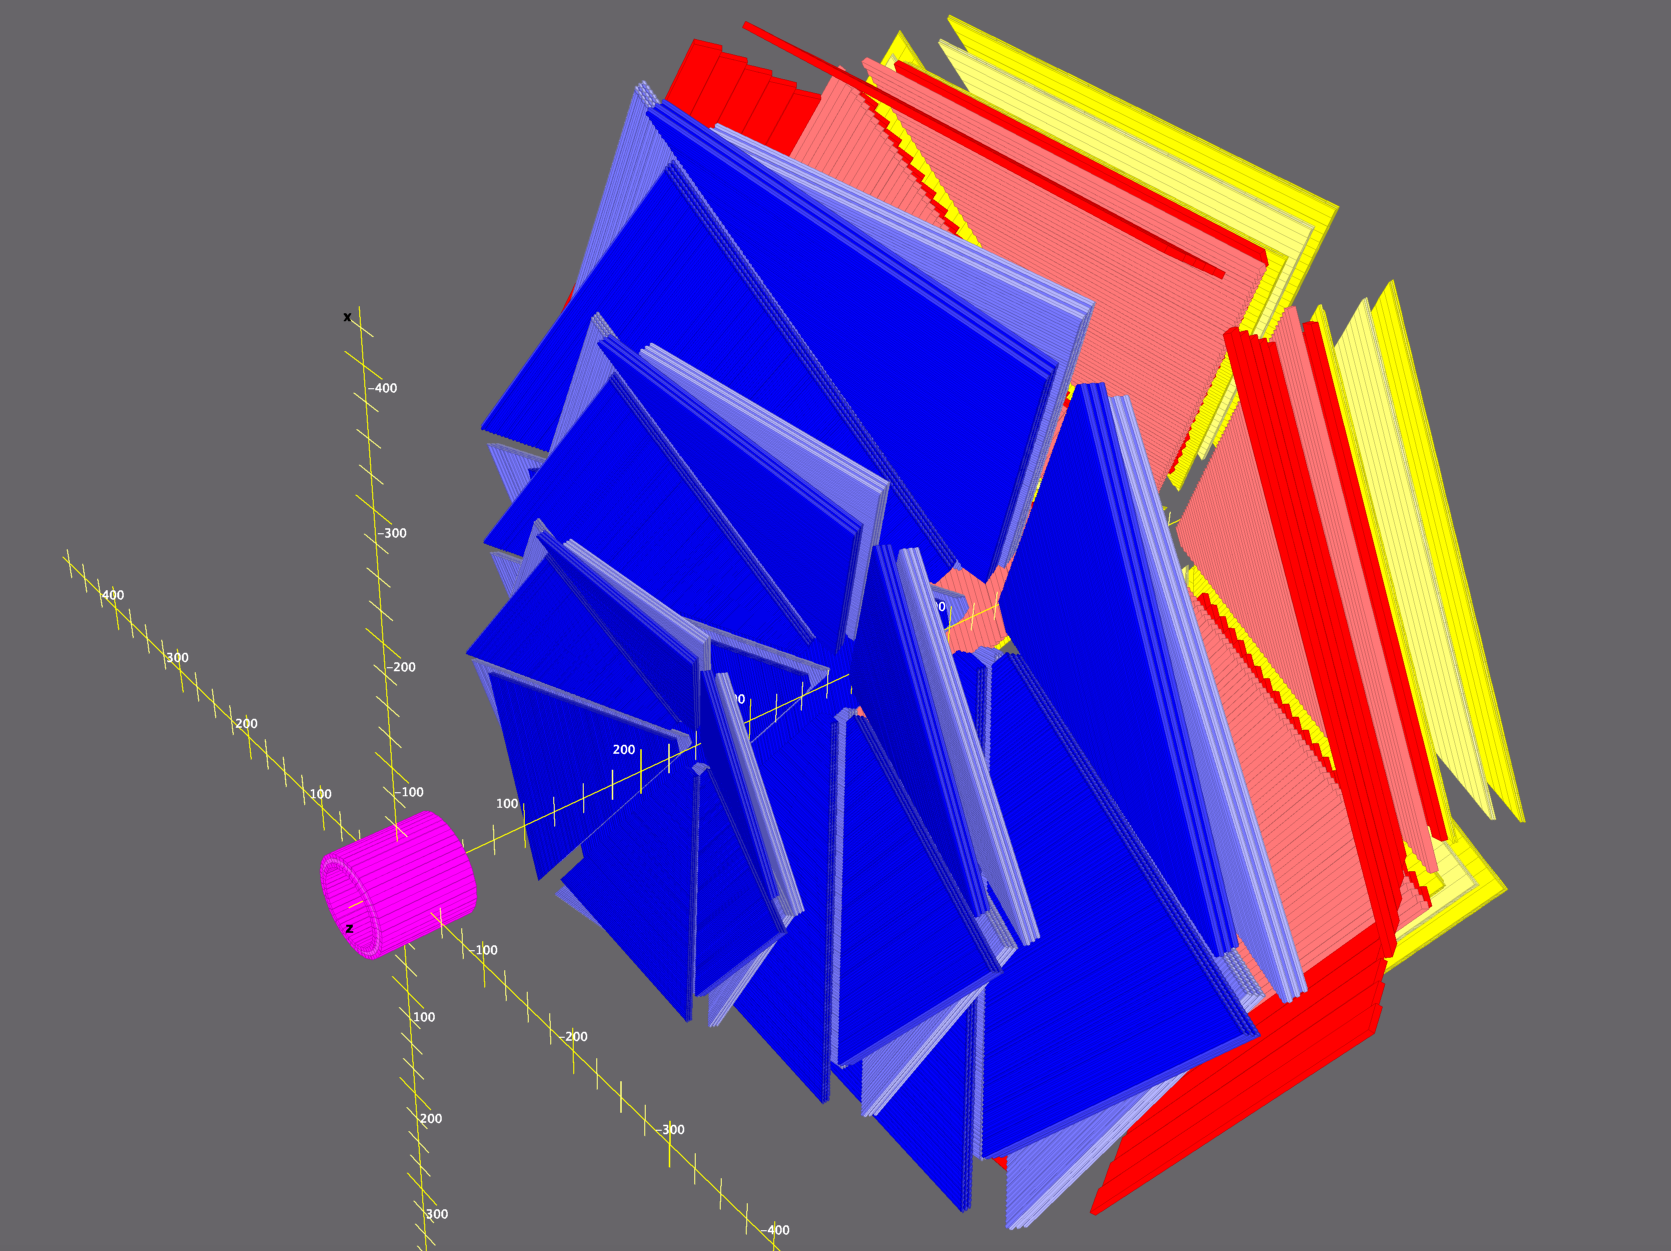
\includegraphics[width=1.0\columnwidth]{reconstruction/pics/detectorview.png}
\caption{Visualization of part of the CLAS12 spectrometer via the geometry package. From left to right, the Central Neutron Detector (CND) in magenta, the Drift Chambers (DC) in blue, the Forward Time of Flight (FTOF) in red, the Electromagnetic Calorimeter (ECAL) in yellow are shown.}
\label{fig:detectorview}
\end{figure}
\subsubsection{Magnetic Field Package}
The magnetic field package {\it magfield} used by CLAS12 reconstruction creates
binary field maps from engineering models of the CLAS12 torus and solenoid. It employs
a common self-described binary format, with a header containing meta-data describing
the pedigree of the field, its grid coordinate system, and the coordinate system
used by the field values. For example, the CLAS12 torus has a cylindrical grid
but Cartesian field components. The same magfield package provides the trilinear
interpolation of the field. Given that the field is often requested at a sequence
of points all contained within a single grid cell, magfield uses time-saving
software “probes” to cache nearest neighbors.

\subsubsection{Swimmer Package}
The swimmer package, in conjunction with the magfield package, is used by the CLAS12
reconstruction to integrate charged particles through the CLAS12 solenoid and torus.
It uses a fourth order (with 5th order corrections) adaptive step-size Runge-Kutta integrator
with single-step advancement achieved through a configurable Butcher tableau advancer.
There are a number of convenience methods for swimming to a plane, to the closest
point on a line, and to a specified value of a given coordinate such as z. For
forward swimming in CLAS12, the swimmer can reduce the dimensionality of the state
vector (and consequently run faster) by changing the independent variable from
the pathlength to the z coordinate.


\section{Data Formats}
\label{sec-formats}

EVIO (Event Input-Output)~\cite{evio} is a data format designed and maintained by the JLab Data Acquisition
Group, and is the data format of the raw data. For event reconstruction and analysis, the CLAS12 data format
was designed to provide a flexible data container structure, with features that minimize disk access for the
most common tasks performed in data analysis. The High Performance Output (HIPO) format developed for
CLAS12 was designed to provide data compression, using LZ4 (the fastest compression algorithm currently
available), and random access.

HIPO stores data in separate records (with adjustable size), with tags associated with each record. Each record
is compressed and a pointer to the record is kept in the file's index table. This feature allows separating events
during reconstruction based on the content of the event, such as the number of reconstructed particles. Users can
read portions of the file depending on the final states to be analyzed.  The meta-data of the file, describing detector
and beam conditions, are common for all analyses.

The HIPO library has both Java and C++ implementations. On the basis of the C++ implementation, a library was
developed extending ROOT base classes to allow for HIPO files to be read from ROOT frameworks. Additional
tools are available to allow users to produce plots using native ROOT syntax.

\section{Calibration}

Since the SVT modules are designed with a binary readout system, the analog channel response cannot be measured directly. Instead, the analog response is reconstructed by injecting a calibration charge on the channel and measuring the corresponding occupancy over a range of threshold values. 

\begin{figure}[hbt] 
	\centering 
	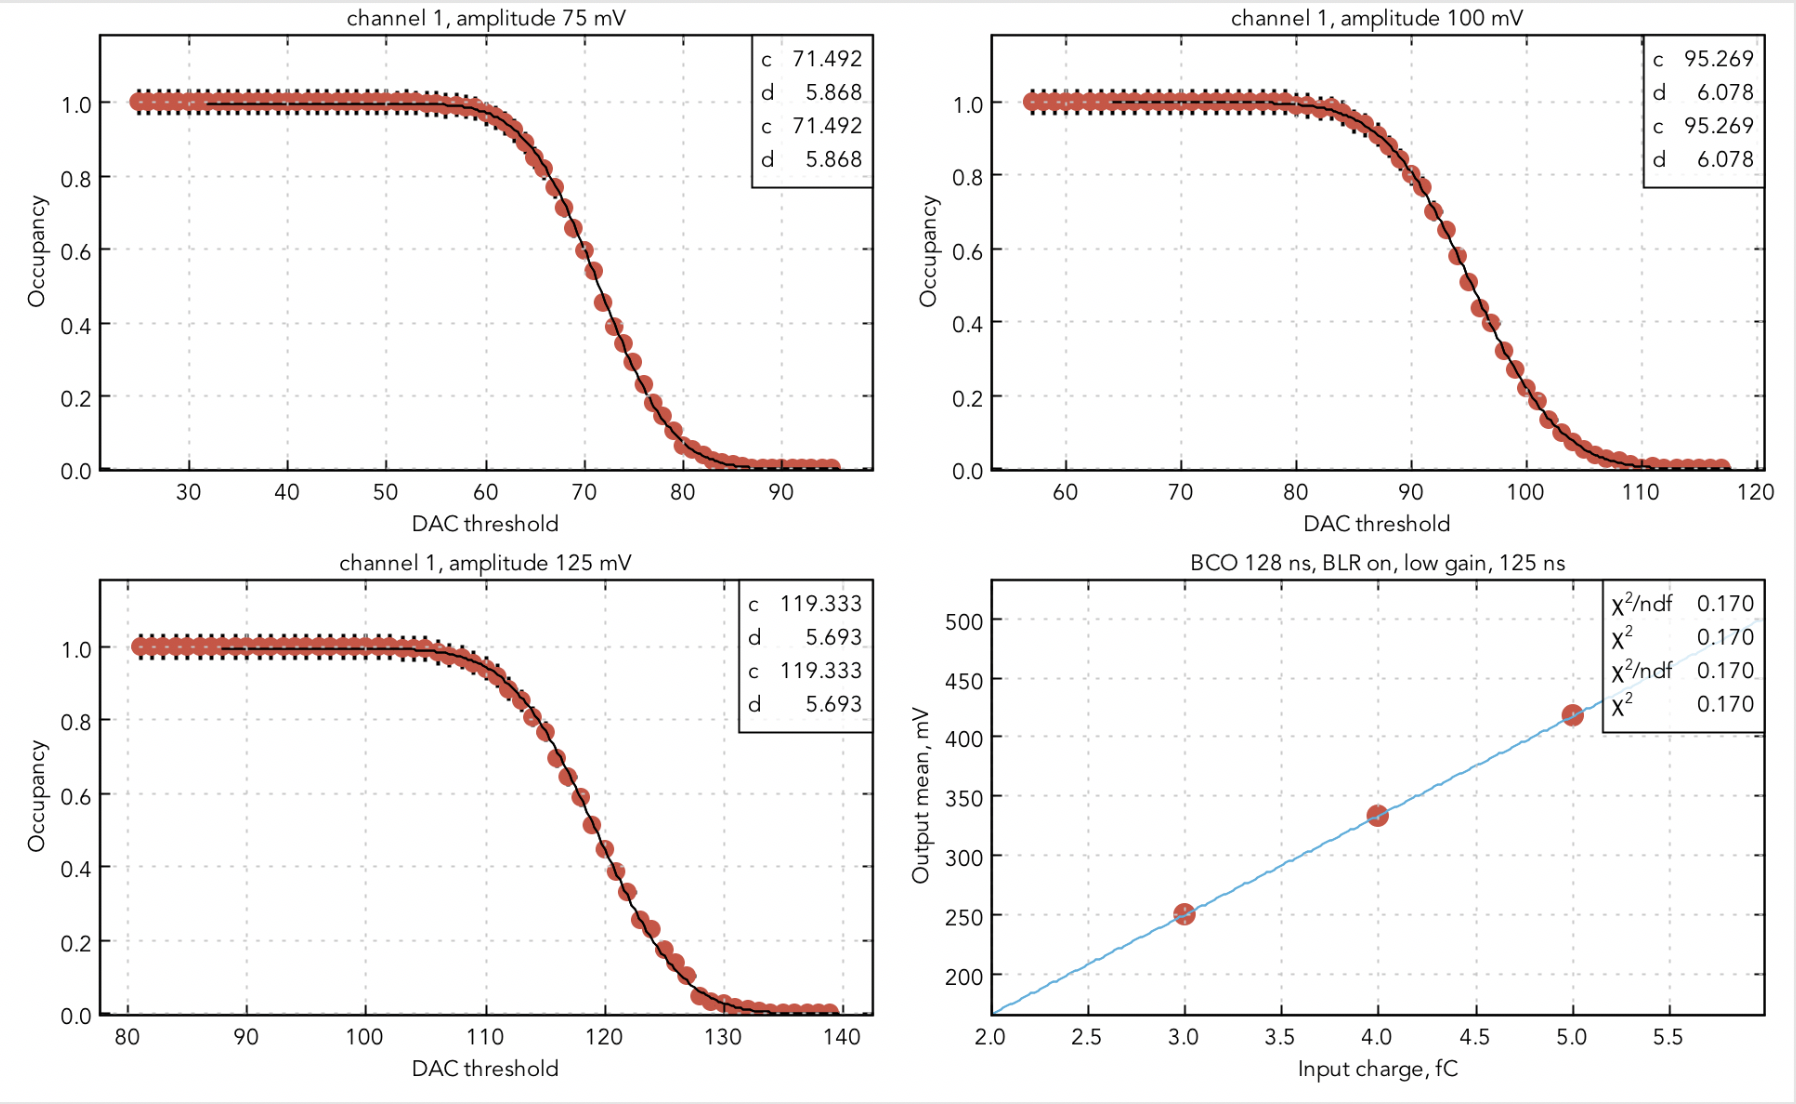
\includegraphics[width=1.0\columnwidth,keepaspectratio]{threshold-scan.png}
	\caption{Threshold scan on a single representative SVT channel.}
	\label{fig:threshold-scan}
\end{figure}

The output signals from the FSSR2 chip can be converted to charge using either internal or external calibration pulses. Because external pulser can be set to higher frequency than internal pulser without affecting the calibration process, external pulser circuit was added to the HBCB and the VSCM. Noise is measured using external, low frequency calibration charge injected in the absence of signal. The injected charge is shaped and amplified in the analog circuitry to form an output signal. The discriminator threshold determines whether or not the output signal corresponded to a hit. The probability that the injected charge produces a hit depends on the setting of the discriminator threshold. The average hit probability is measured by repeating the process of injecting charges and counting the fraction of readout triggers that produced a hit. This measurement is repeated over a range of threshold settings to produce an occupancy plot. 

The occupancy plots are measured setting the pulser amplitude at fixed values and changing the comparator thresholds. Each point of an occupancy plot represents the percentage of times that the comparator fires for a certain value of injected charge. In Fig.~\ref{fig:threshold-scan} presented three occupancy plots taken at different pulser amplitudes and the response plot showing the linear dependence of the output pulse height on the input charge in the operation region of the preamplifier. In between the high and low threshold regions, the occupancy curve is described by an error function, or S-curve, which can be fitted to the occupancy histogram for each channel, producing a mean value (discriminator threshold) and standard deviation (noise). The conversion from mV to electrons is performed considering a nominal value for the FSSR2 injection capacitance of 40~fF. 

\begin{figure}[hbt] 
	\centering 
	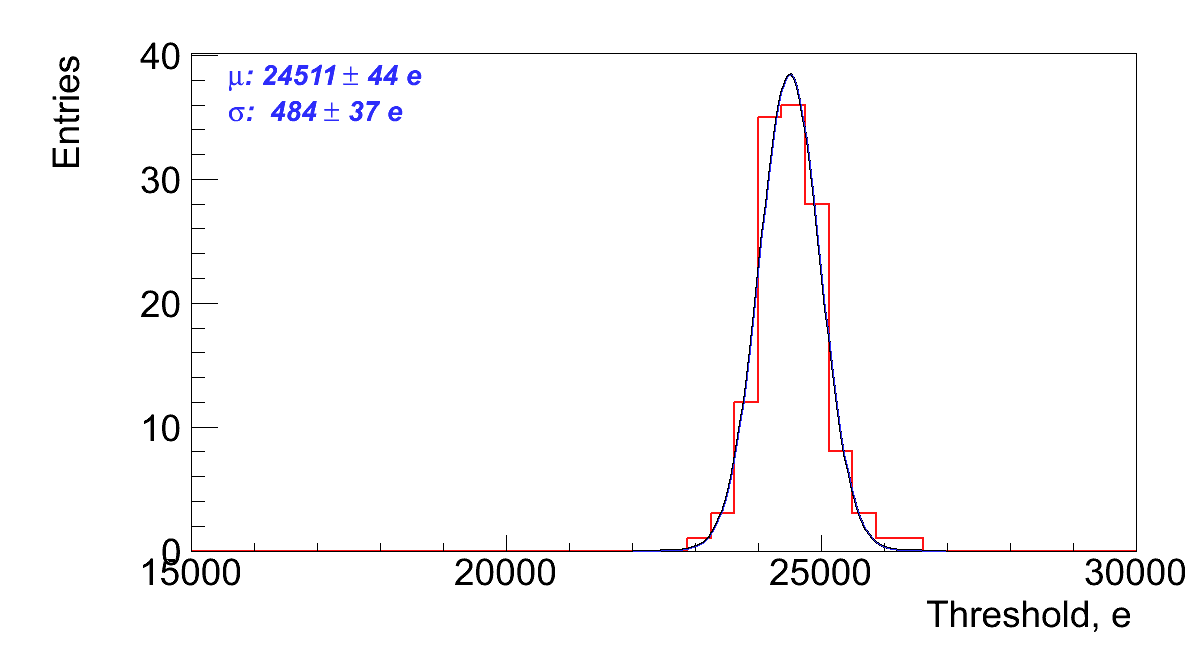
\includegraphics[width=0.8\columnwidth,keepaspectratio]{thrdisp.png}
	\caption{Typical threshold dispersion within a chip.}
	\label{fig:thrdisp}
\end{figure}

Threshold charge must be the same across the channels in a detector, otherwise the track-finding algorithms would be biased by the potential extra hits. Any spread in the response among the different channels of a chip results in a spread of the efficiency and noise occupancy which degrades effective performance. This leads to a requirement that the channel-to-channel variations in threshold and noise are kept to a minimum. Threshold dispersion is defined to be a standard deviation of the distribution of means obtained from the parameters of the complementary error function fit. The noise and threshold dispersion constants for each individual detector channel are measured and the values are used by the zero-suppression algorithms implemented in the core logic of the FSSR2 and by calibration procedures to identify defective channels. A comparison of the noise for 33~cm strips with the threshold spread demonstrates that the threshold spread is negligible compared to the noise and does not affect the efficiency and noise occupancy (see Fig.~\ref{fig:thrdisp}). The threshold dispersion agrees with expectations for the FSSR2 chip for the chosen settings.

SVT calibration data are stored in CLAS12 calibration database. The channel calibration table has columns corresponding to sector, layer, chip ID, mean, channel status (good, noisy, open, dead, or masked), ENC, gain, offset, V$_{t50}$ (threshold at 50$\%$ occupancy), and the threshold. There are 21504 rows in the channel calibration table. The ENC and gain are calculated using a calibration amplitude equal to 100 DAC.
The chip calibration table has columns corresponding to layer, sector, chip ID, ENC (electrons), gain (mV/fC), offset (mV), the threshold at 50$\%$ occupancy (V$_{t50}$, mV), threshold dispersion (electrons), chip gain (low, high), BLR mode (off, on), BCO time (ns), shaper time (ns), 8 ADC thresholds in DAC. There are 168 rows in the chip calibration table. 


\section{Event Reconstruction}

Reconstruction of the FT sub-detector information and the matching between the detectors to determine the type and
three-momentum of the incident particles is implemented in the CLAS12 Java reconstruction framework. Details on
the algorithms and implementation are provided in Ref.~\cite{reconstruction}. In the following we briefly summarize
the main steps and final outputs.

FT-Cal hits are reconstructed from the analysis of the recorded FADC information to extract energy and time;
hits are then associated based on position and time to form clusters whose energy and centroid position are used
as an initial seed to define the three-momentum of the incident particles. Similarly, FT-Hodo hits are reconstructed
from the FADC raw information and matched based on position and timing to form clusters of matching tiles in the
two layers of the detector. These are matched to clusters in the calorimeter based on position and time to distinguish
charged particles from neutrals. Finally, FT-Trk hits are also reconstructed from the raw data and geometrically
grouped to form clusters in each of the detector layers separately. Combinations of clusters in the $x-y$ layers of
each of the two sub-detectors are used to define crosses that are finally matched to calorimeter clusters to improve
the determination of the impact point of the particle.


\subsection{Tracking Overview}
The reconstruction program must reconstruct, on an event-by-event basis, the raw data coming from either
simulation or the detectors to provide physics analysis output such as track parameters and particle
identification. Charged particle tracking is separated into the reconstruction of tracks in the central
(Silicon and Micromegas Vertex Trackers) and forward (Forward Micromegas Tracker and Drift
Chambers) detectors. The forward region covers the angular range from $5^\circ$ to $40^\circ$, while
the Central Detector covers approximately $40^\circ$ to $135^\circ$. In the central region a 5~T
solenoidal magnetic field bends charged tracks into helices, while forward-going tracks are bent by a
$\sim$2~T toroidal magnetic field. For both systems, track reconstruction comprises algorithms for
pattern recognition and track fitting. Hit objects, corresponding to the passage of a particle through a
particular detector component, require the transformation of an electronic signal into a location of the
track's position in the detector sub-system geometry. A hit is thus a geometric object, for example, a
line segment. These objects then form the input to the pattern recognition algorithms. This first step
involves the identification of clusters of hits and the determination of the spatial coordinates and
corresponding uncertainties for hits and clusters of hits. At the pattern recognition stage, hits that are
consistent with belonging to a trajectory (i.e. track) are identified. This set of hits is then fit to the
expected trajectory with their uncertainties, incorporating the knowledge of the detector material and
the detailed magnetic field map.

CLAS12 has a unique magnetic field configuration that involves tracking though both a solenoidal and toroidal field. Tracks reconstructed in the forward detector are fit in the forward tracking detectors and subsequently swam to the beam line through both fields.  A view of the field intensities in the $(z,x)$ plane and overlap region for the torus and solenoid fields is shown in Fig.~\ref{fig:fields}.

\begin{figure}
\centering
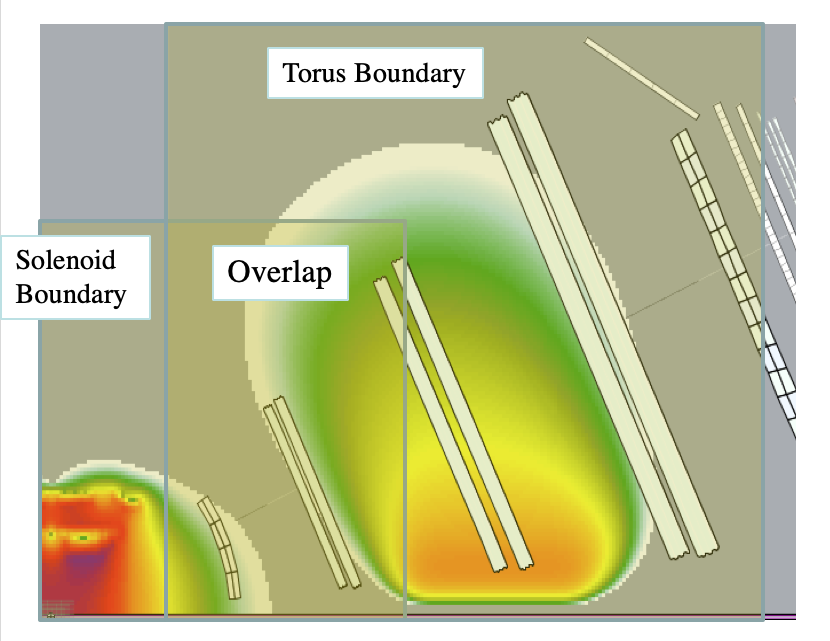
\includegraphics[width=0.5\textwidth]{pics/Bfields.png}
\caption{Event display of the CLAS12 magnetic fields. 
}
\label{fig:fields}
\end{figure}

\subsection{Forward Tracking}

\subsubsection{Hit Reconstruction}

The Drift Chamber (DC) wire hit information is given by the wire geometrical location and the drift time
to the wire. Track-dependent corrections to the hit, such as left-right ambiguity and time-walk must then
be performed. 
Pattern recognition for the DC is priori done using only wire position information and searching for groups of hits forming clusters.  This portion of the algorithms is called ``hit-based'' tracking.  In hit-based
tracking, a hit is defined as a wire with a recorded signal.  No timing information is incorporated at the
preliminary stage of the reconstruction.  
After a ``hit-based''  track has been found, corrections to the raw TDCs of the hits on track resulting from the propagation time along the hit wire, the signal time of flight, the event start time and the cable delays are applied to determine the hit time.  A distance of closest approach (DOCA) to the hit wire is estimated from the time.  At this stage the tracking is redone using the calculated DOCAs in order to fit the track (see Fig.~\ref{fig:docas}.  This portion of the DC reconstruction phase is called ``time-based'' tracking.  The calibration parameters entering in the function used to convert distance to time that is inverted in reconstruction (see Ref. DC paper) are extracted from the distance of local fits to the DOCAs using a linear function to the wire position. 

\begin{figure}
\centering
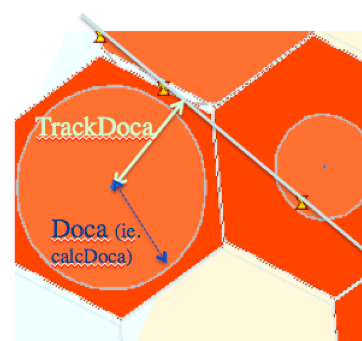
\includegraphics[width=0.2\textwidth]{pics/dcPattern10.png}
\caption{
Illustration of DOCA computed from the corrected time and of the distance from the wire to the track (TrackDoca).
}
\label{fig:docas}
\end{figure}

In hit-based
tracking, uncorrelated hit noise in the DC are identified by a Simple Noise
Removal (SNR) algorithm and rejected. SNR stores all the data for a drift chamber layer (112 sense wires)
bitwise in an extended 128-bit word, with "set" bits corresponding to hits. The algorithm is configured
through parameters specifying the maximum tilt of a track segment and the number of missing layers
allowed in the formation of a segment. Using bitwise operations on the extended words, the algorithm
essentially operates as a parallel processor on all 112 sense wires in layer. This parallelism precludes the
need of a wire for-loop, enabling the algorithm to run in a negligible fraction of the total time for
reconstruction. More to the point, SNR actually saves time by reducing the combinations that must be
explored in the pattern-recognition phase of the ensuing track-finding.
An illustration of the SNR hit categorization in the DC is displayed in Fig.~\ref{fig:snr}.
\begin{figure}
\centering
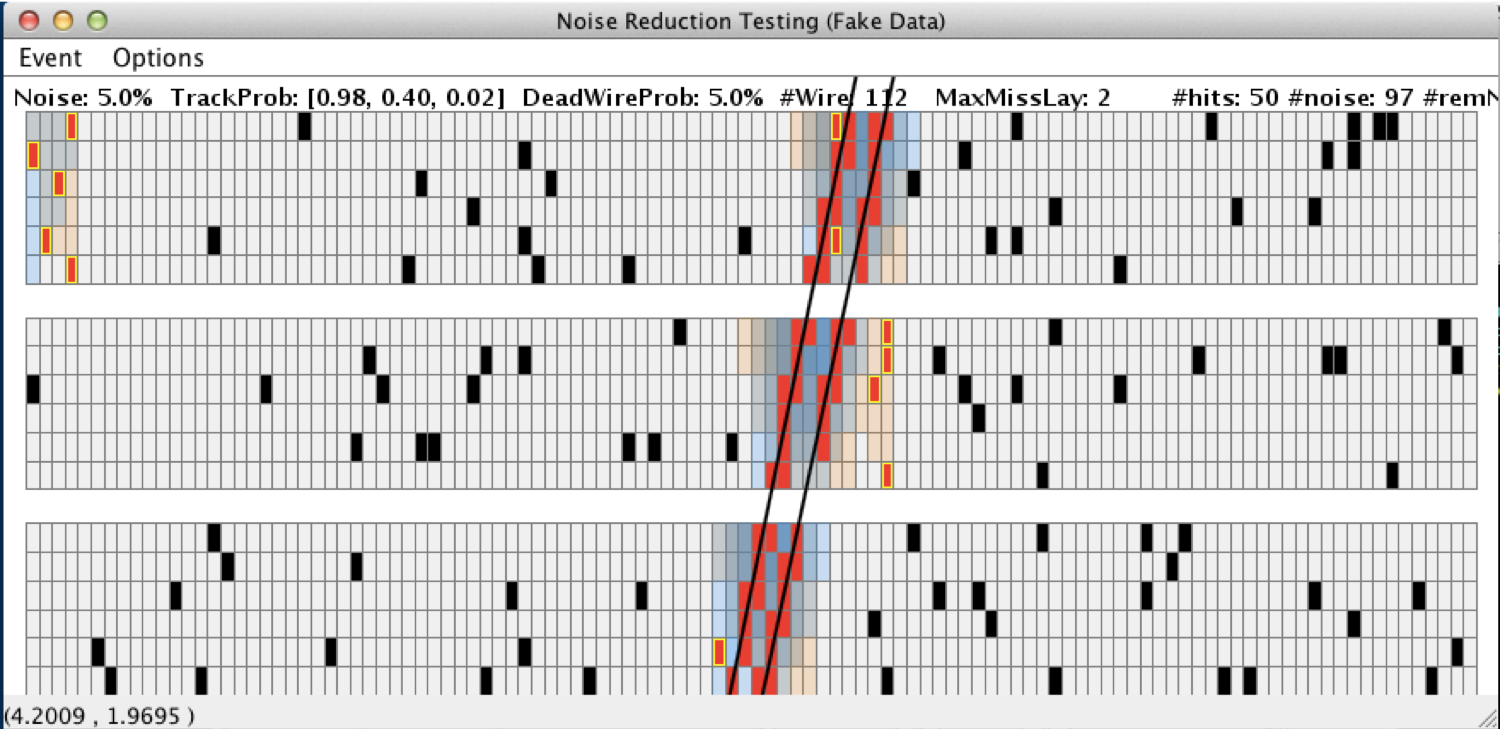
\includegraphics[width=0.48\textwidth]{pics/dcPattern9.png}
\caption{
Illustration of DC hits categorized by the SNR algorithm.  
Black hits are identified as noise and discarded.
Red hits are saved for further evaluation by the subsequent hit selection algorithms. 
Red hits with yellow frames are saved noise (false alarms).  Shaded areas correspond to 
possible clusters.  The darker shades correspond to a higher quality factor, hence a higher probability for hits on track.
}
\label{fig:snr}
\end{figure}

\subsubsection{Hit Clustering}
The hits remaining after the SNR
algorithm are grouped into clusters.
Clusters are groups of adjacent hits in a group of 6 layers forming a DC superlayer.  There can be at most
two hits in a layer, forming a ``double-hit''~\footnote{An additional hit in a layer is mostly out of time and has 
a drift time that when converted to a drift distance exceeds the cell size. }  However, up to four layers can be missing in a superlayer
when attempting to form a cluster.  This is to reduce tracking inefficiencies resulting from possible wire malfunctions or
intrinsic inefficiencies. It was found that using 4 out of 6 layers to form a cluster is good enough
to determine the cluster shape which is subsequently used in tracking to determine the track trajectory. 
\begin{figure}
\centering
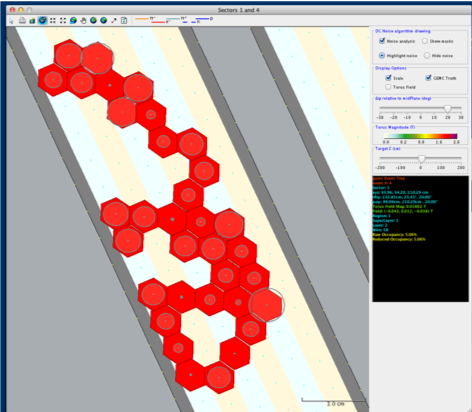
\includegraphics[width=0.4\textwidth]{pics/elooper.png}
\caption{
Illustration of typical noise patterns in the DC displayed with the CLAS12 Event Display (CED). 
The hits shown in the display correspond to electrons from a MC sample.
}
\label{fig:eloop}
\end{figure}

Additional ``noise rejection'' algorithms are applied to the clusters to remove spurious hits
that do not come from a real track. 
So-called ``curlers'' patterns as show in Fig~\ref{fig:eloop} are typical for low energy electrons  in the DC.   So a pruning algorithm was designed to remove them at an early stage of the reconstruction. The  algorithm is a counting method of the number of contiguous hits in a layer of a superlayer.  In Figs.~\ref{fig:eloop} and ~\ref{fig:strings} we also see another typical noise pattern that looks like horizontal ``strings'' of hits along a layer.  The algorithm was developed following  the observation that high-momentum tracks from hadrons typically cross the superlayers at a large angle,
while ``curlers'' from low-momentum background follow curling trajectories with a significant part of the
pattern being along layers.
Subsequent algorithms  are employed for resolving overlapping segments.   
\begin{figure}
\centering
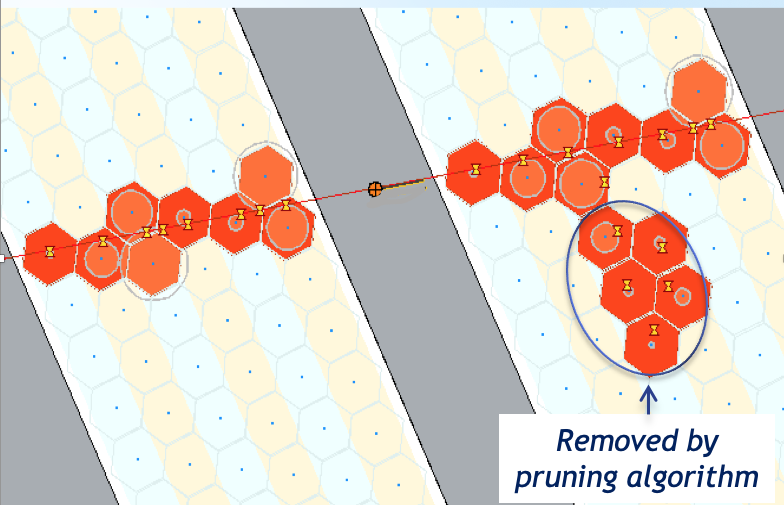
\includegraphics[width=0.4\textwidth]{pics/dcPattern2.png}
\caption{
Illustration is hits rejected by the pattern recognition algorithm in a MC sample corresponding to electron tracks generated at 4.5 GeV at the center of the sector ($\phi = 0\deg$ with a polar angle of $10\deg$. 
The circles superimposed on top of the DC cells indicate the DOCAs computed from the fully corrected times.  The yellow hourglass symbols show the simulated track positions along the trajectory.   
The algorithm looks for ``strings'' of hits such as shown in the the third column of hits in the right-most superlayer in the figure.  
In this instance, the middle hit would be rejected, leaving a set of four attached hits which would subsequently be rejected since they would no longer be attached to the main cluster. 
}
\label{fig:strings}
\end{figure}


Overlapping segments are produced when the trajectories of tracks cross each other
or when the tracks are almost parallel and very close to each other in a given region.
A Hough transform is employed to find hits on a line in the cluster which allows splitting the cluster into
segments.  The resulting trimmed clusters are then fit to a straight-line hypothesis, and those hits with
acceptable residuals are kept and identified collectively as a ``track segment''. An illustration of the Hough Transform cluster selection algorithm is shown in Fig.~\ref{fig:hough}.

Subsequent hit pruning algorithms are employed at ``time-based'' level.  
Figure~\ref{fig:dcsegs} illustrates the selected hits belonging to a cluster (orange) and the hits
rejected by the noise-finding algorithms.

\subsubsection{Pattern Recognition}
Fits to the segments with a linear function are a preliminary step to estimating
a track trajectory. Track parameters are estimated in the local coordinate system of the chamber sector from
this trajectory.

\begin{figure}
\centering
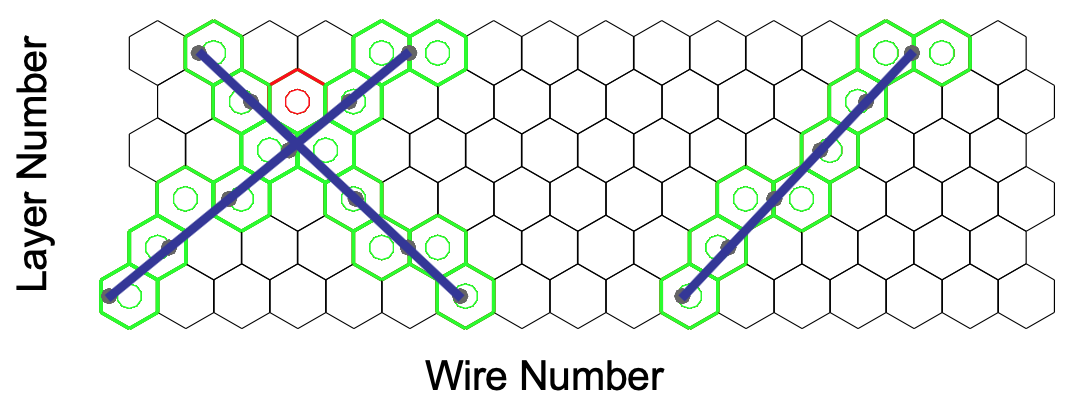
\includegraphics[width=0.45\textwidth]{pics/dcPattern14.png}
\caption{
Illustration of selected clusters (left-most selected hits with superimposed lines) using a Hough Transform.  Two track segments cross each other.  The hits are separated into cluster candidates and fit using a local coordinate system as a function of layer and wire number.  The selection is done without employing timing information. 
}
\label{fig:hough}
\end{figure}
Using the wire direction in a given superlayer along with the line fit to a segment in that superlayer, a plane can be constructed.
Thus pairs of segments in
neighboring superlayers within one chamber (with superlayers of $\pm$6$^\circ$ stereo angle) represent the
intersection of two planes, that is a line whose coordinates are evaluated midway between the two
superlayers, and is a 6-dimensional object (x,y,z and 3 angles) which we call a ``cross''.
A segment slope coincidence algorithm is used to match neighboring segments in a region (see
Fig.~\ref{fig:dcsegs}).  Selection cuts are subsequently applied on the
reconstructed cross to ensure that it is within the fiducial sector volume within resolution.

\begin{figure}
\centering
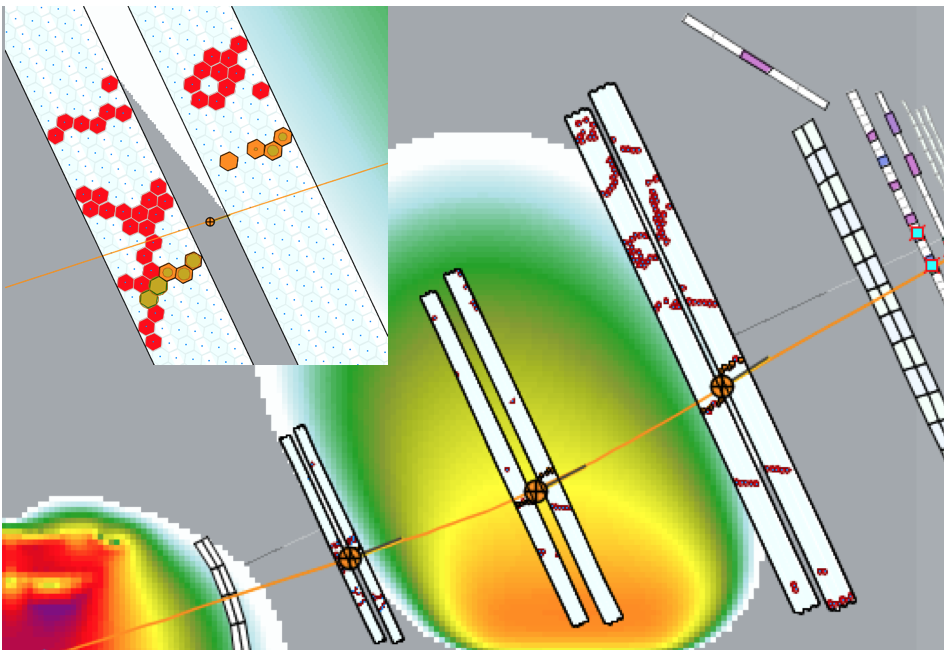
\includegraphics[width=0.4\textwidth]{pics/dcPattern13.png}
\caption{
Illustration is hits (red hexagons) rejected and accepted (orange hexagons) by the pattern recognition algorithm in a MC.  
The red cells correspond to hits not rejected by the SNR algorithm.  The circles represent the calculated DOCAs.  The superimposed lines show the local fits to the DOCAs.  The filled circle in the middle of the two superlayers represents the 3-dimentional point (i.e. ``cross'') obtained from the local fits to the DOCAs taking into account the direction along the wires.
The offset between the segments composing the cross comes from the projection at the $y=0$ plane (midplane).
The cluster shown on the right-most superlayer is an example of a ``looper'' and shows how this category of cluster has the potential to bias the track.  The second cluster used to form the cross yield an incorrect slope resulting from a wrong hit used in the fit.  Subsequently, the ``looper'' searcher algorithm rejects the entire cluster and only the first cluster is used to fit the track.  The fitted track trajectory is represented by the orange line. 
The upper figure is a zoomed view into the track trajectory in region 1.
}
\label{fig:dcsegs}
\end{figure}


An additional  pattern reconstruction algorithm  matches segments within even and odd superlayers, respectively, to form
a track candidate where an entire superlayer can be missing.  The matching algorithm returns an estimates of where the missing
superlayers hits should be and forms a pseudo-segment from the wire locations corresponding to these hits.  Subsequently
a pseudo-cross is formed using the pseudo-segment and the neighboring reconstructed segment in that region.

The first stage of
pattern-recognition consists of finding a track candidate, from a set of 3 crosses (one each in R1, R2 and R3) that
are fit to a parabolic functional form to give us a ``track candidate''.
Using the parameters of the parabolic function between the first and the third cross and obtaining the magnetic field
intensity at each step along this trajectory we obtain an estimate for $\int B dl$.
From the local angles of the crosses in the $x-z$ plane for R1 ($\theta_1$) and R3 ($\theta_3$) we estimate the track momentum ($p$)
and the particle's charge ($q$),
as follows:
\begin{equation}\frac{q}{p} = \frac{\theta_3 - \theta_1}{v\int{B dl}},\end{equation} where the angles are in radians, the magnetic field
intensity ($B$) is in Tesla, and the pathlength ($dl$) in cm.
The conversion factor  $v = 0.002997924580 (GeV/c) T^{-1} cm^{-1}$  corresponds to the speed of light.
The cross position and angles in region 1 together with the
momentum and the charge provide all the necessary information to define the track parameters at a given location in the detector,
and therefore to start track fitting.


\subsubsection{Track Fitting}
The output of the pattern recognition
is a seed with initial parameters used to start the track propagation from one measurement site to the next in the fit.
Track fitting uses a Kalman Filter method with a 5-parameter track representation ($x$, $y$, $tx$, $ty$, $q$/$p$), defined
in a local coordinate system with the z-axis perpendicular to the chambers wire planes; where $q$ is the
track charge, $tx=px$/$pz$,
$ty=py$/$pz$, with $px,py,pz$ resenting the $x,y,z$ components of the track momentum in that (analysis) frame.
In the analysis frame the state vector (representing the track parameters) and the measurement are defined at each layer
at which there is a hit on track.
Hence, as in ref~\cite{spiri} we can express the equations of motion of the track in the torus field
and the propagation of the state vector covariance matrix as derivatives with respect to $z$.
In the drift chambers, the magnetic field components are mostly along the $y$ coordinate in the analysis frame.
The trajectory of the particle in the analysis frame is given by the following equations:

\begin{eqnarray*}
%\systeme{
dx/dz  &=& tx, \\
dy/dz  &=&  ty, \\
dtx/dz &=& q \cdot v \cdot \sqrt{1 + {t_x}^2 + {t_y}^2}\cdot [t_y\cdot (t_x B_x + B_z)\\ &-& (1 + {t_x}^2 ) B_y], \\
dty/dz  &=&  q \cdot v \cdot \sqrt{1 + {t_x}^2 + {t_y}^2}\cdot [-t_x\cdot (t_y B_y + B_z) \\&+& (1 + {t_y}^2 ) B_y], \\
q  &=&  q_0,
%}
\end{eqnarray*}


where, and the initial values at the initial plane $z = z_{0}$ are
$x = x_{0}, y = y_{0}, t_x = t_{x0}, t_y = t_{y0}, q = q_{0}$.

we solve the above equations
numerically using a fourth order Runge-Kutta integration method in order to propagate the state vector from
the drift chamber plane at $z_{0}$ to the next one at $z$.  The state covariance matrix is propagated along with it
by computing the Jacobian matrices as in ref~\cite{spiri} (again, solving using a fourth order Runga-Kutta method).
The Jacobian matrix terms contribute to the propagator matrix used to compute the Kalman gain.
The propagated covariance matrix takes into account multiple scattering.

The non-zero components of multiple scattering matrix are:
\begin{eqnarray*}
Cov (t_{x} , t_{x}) &=& (1+{t_x}^{2} )\cdot (1+{t_x}^{2} + {t_y}^2 )\cdot {\theta_{0}}^{2} , \\
Cov (t_{y} , t_{y}) &=& (1+{t_y}^{2} )\cdot (1+{t_x}^{2} + {t_y}^2 )\cdot {\theta_{0}}^{2} , \\
Cov (t_{x} , t_{y}) &=&  t_{x} t_{y}\cdot (1+{t_x}^{2} + {t_y}^2 )\cdot {\theta_{0}}^{2} ,
\end{eqnarray*}
where,
\begin{eqnarray*}
{\theta_{0}} &=& \frac{13.6}{\beta pc}\sqrt{\frac{t}{X_{0}}\sqrt{1+{t_x}^2+{t_y}^2}}\\ &\times&\left[ {1+0.038 ln \left({\frac{t}{X_{0}}\sqrt{1+{t_x}^2+{t_y}^2}}\right) }\right].
\end{eqnarray*}
as given by the Highland-Lynch-Dahl formula [ref.].
The radiation length $X_0$ is computed as an effective radiation length corresponding to the gas mixture in the DC.
Air is assumed outside of the DC volumes. The term $t$ represents the pathlength traverse by the track.

At each plane the state vector is mapped onto a measurement, which corresponds to the drift distance to the
wire at a given drift chamber plane.  In instances where there are two hits in a given wire (i.e. the track
goes in between the wires), the information from both hits is included in the fit.
The measurements used in the fit
take into account the left/right position of the track with respect to the wire.

Time corrections are applied
after ``hit-based'' tracking to account for the event start time, cable delays, propagation times along the
wires, event flight times to the hit location along the wires, beta-dependent corrections, and the effect of
the magnetic field on the cell isochrones which modify the drift times.

After the times are corrected, the drift distance is computed using a tabulated distance-to-times
multi-dimentional arrays.  The drift distances are computed using a multi-dimentional interpolation method
using the segment local angle, the value of the magnetic field at the location of the hit and the corrected
times.  The Kalman fit is redone at ``time-based'' level using hits with corrected times and computed drift
distances.

A graphical representation of tracks in the CLAS Event Display is shown in Fig.~\ref{fig:dcTracks}.  
This is a typical event for the nominal running conditions for CLAS12.  The
display shows a longitudinal view of the chambers trapezoidal shapes. The field intensity is represented by a
color gradiant. The drift chamber hits correspond to the maroon shapes.  The bottom track goes through a
characteristic noise pattern in Region 1 (R1). Only the first superlayer in R1 is used to fit this track.  The
tracks hit the Forward Time-Of-Flight system and the Calorimeters.  The top track leaves a hit in the HTCC
and is identified as an electron (see section on the event builder).

\begin{figure*}
\centering
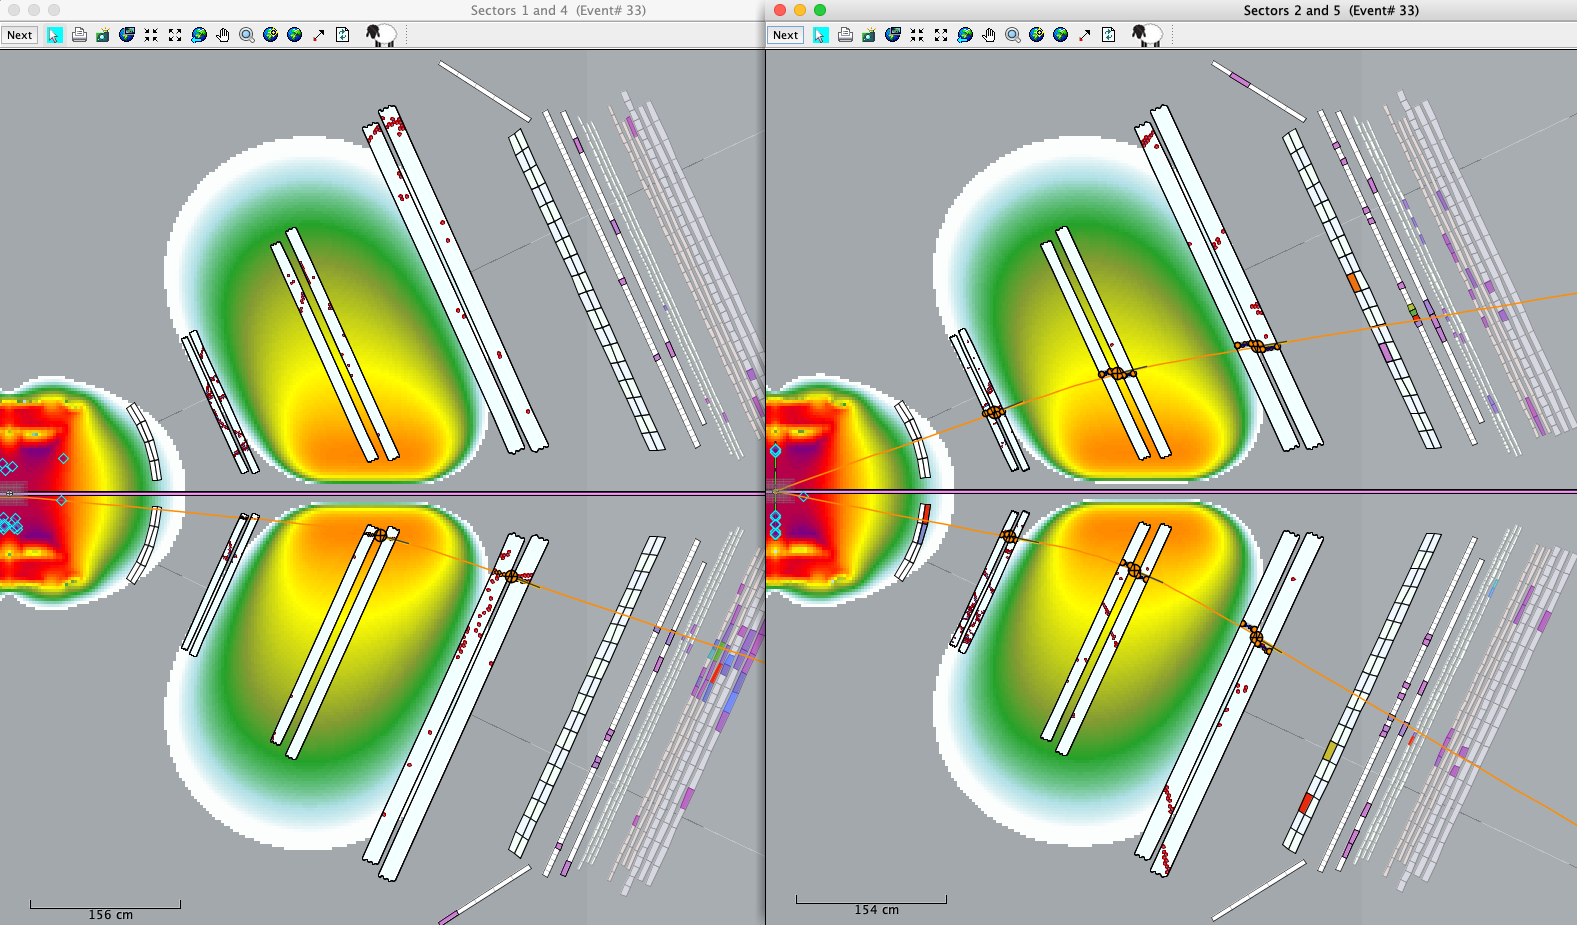
\includegraphics[width=0.95\textwidth]{pics/dcTrack3.png}
\caption{Event display of charged particle tracks in the Drift Chambers.  The reconstructed 
track in the bottom left view is an example of the use of the five-out-of-six-superlayer tracking. 
The second superlayer segment is missing in this case.  The track on the bottom right is identified 
as an electron and leaves a hit in the HTCC (red shape at the exit of the solenoid. 
}
\label{fig:dcTracks}
\end{figure*}

\subsection{Artificial Intelligence Assisted Forward Tracking}
\subsubsection{Motivation}
Recent progress in machine learning field offer a promising alternative to conventional
algorithmic tracking methods. While the conventional
methods provide algorithms that are well understood and well studied, there are some algorithms
in data reconstruction process that can be substituted with neural networks to reduce data
processing times. For CLAS12, tracking is the most time consuming process in experimental data processing.
Tracking in the DC takes up to 94\% of total data processing time, which includes finding
track candidates and iterating through track forming segments combinatorially to find the best
combinations of segments that can form a track. This time increases with luminosity as noise
segments increase and can lead to processing time degradation with higher luminosity. We have started 
to address this issue by employing machine learning techniques to find best track candidates in
each event and reduce the number of combinatorics.
\begin{figure*}
\centering
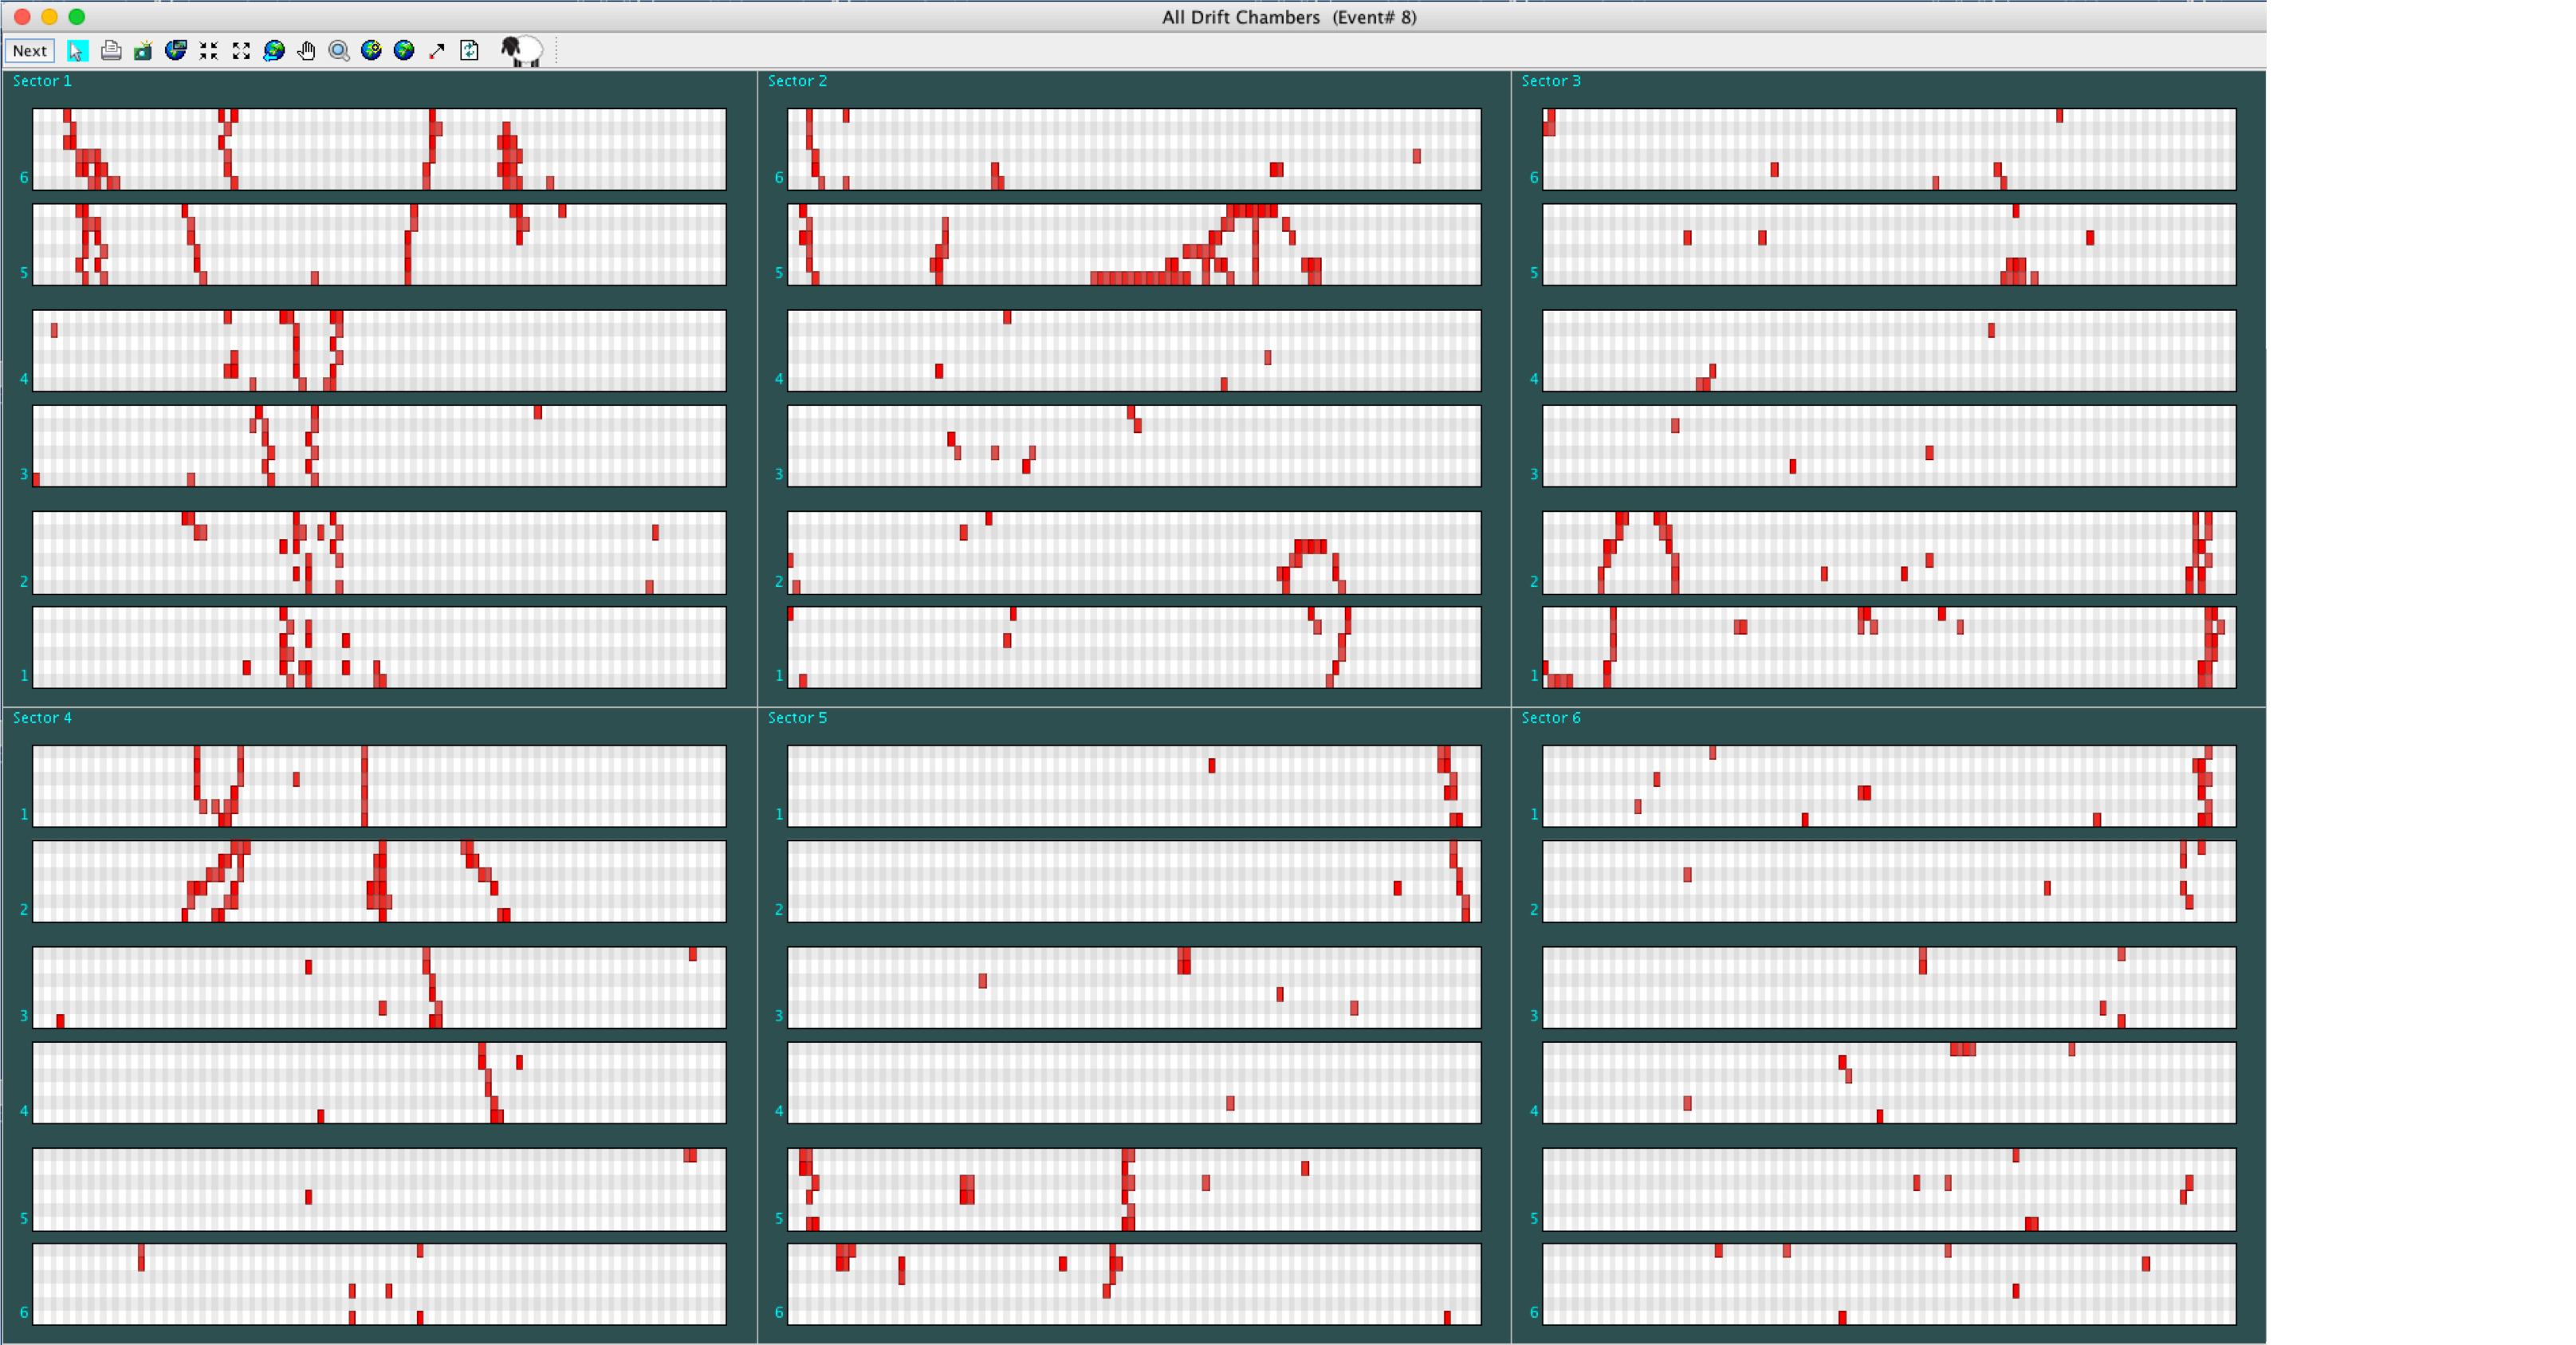
\includegraphics[width=0.95\textwidth]{pics/nn1.png}
\caption{Event display of track segments in the DC. 
}
\label{fig:nn1}
\end{figure*}
\subsubsection{Development}
With increased luminosity the number of potential DC cross candidates
increases.  This implies that the  Kalman Filter fitting algorithm must be run for all possible
combinations crosses.  Fig.~\ref{fig:nn1} shows a typical example of drift
chamber data is shown in a longitudinal projective view using CED. 
This figure illustrates the potential of combinatorial trials to identify tracks. 
We are developing a classifier convolutional neural network that can
identify which segments from each region of CLAS12 drift chambers can potentially form a
good track. We intend to use this network in reconstruction process to reduce the number of
combinatorial fitting.
Reconstructed track segments from both positive and negative tracks from the currently reconstructed data samples are used to train the Neural Network. 
We are currently testing three types of Neural Networks: boosted decision tree, multilayer perceptron, convolutional neural network.  
The accuracy of the network is measured using 4 quantities:
\begin{itemize}
\item{The ratio of valid tracks (correctly detected) to the total number of tracks in the sample. }
\item{The ratio of valid tracks and  invalid tracks (miss-predicted as valid ones; i.e. False Positives) to the total number of tracks in the sample. }
\item{The ratio of valid tracks (correctly detected with highest probability) to the total number of tracks in the sample. }
\item{The ratio of invalid tracks (False Positives) to the total number of tracks in the sample. }
\end{itemize}
Accuracy scores where determined for different training set and for the 3 types of Neural Networks studied.  Preliminary results indicated that the Convolutional Neural Network performed competitively with the Multilayer Perceptron with about 97\% accuracy and 3\% False Positives. 

The hits identified as On-Track by the Neural Network are saved in a bank and the DC reconstruction package was adapted to read these data as an input to hit-based tracking.

Benchmark results of reconstruction speed for hit-based tracking are shown in Fig.~\ref{fig:nn2}

\begin{figure}
\centering
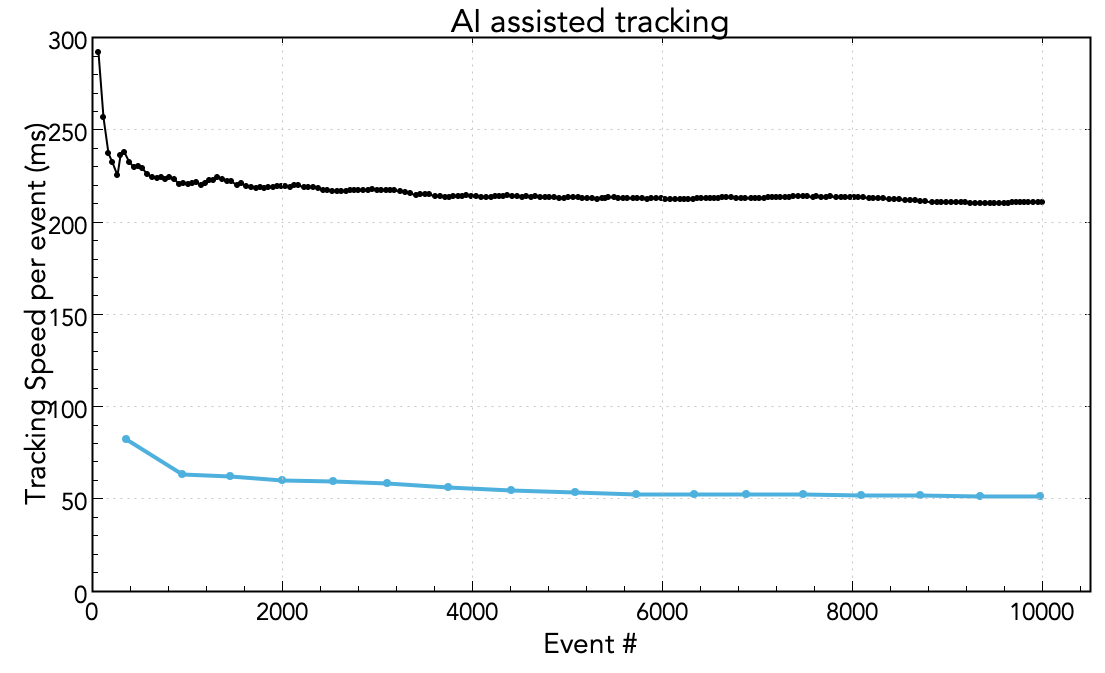
\includegraphics[width=0.5\textwidth]{pics/nn2.png}
\caption{Benchmark results of reconstruction speed for hit-based tracking.  
The (black) blue curve correspond to the (non) AI-assisted reconstruction processing time as a function of event number. 
}
\label{fig:nn2}
\end{figure}

The implementing the Neural Network software into the CLAS12 reconstruction workflow is under development. The second stage of the Machine Learning project will concentrate on efficiency improvements using AI-assisted tracking.

\subsection{Central Tracking}\label{sec:cvt}

Tracks whose angle with the beam direction is between $40^\circ$ and $135^\circ$ are reconstructed by the so called
Central Vertex Tracker (CVT). The CVT consists of twelve cylindrical layers of tracking detectors, numeroted from 1 for
the most inner layer to 12 for the most outer layer. The subset of tracking detectors forming layer 1 to 6 are silicon
strip detectors and will be referred as the Silicon Vertex Tracker (SVT) described in~\cite{svt-nim}. The layers from 7
to 12 are made of micromegas detectors and will be referred as the Barrel Micromegas Tracker (BMT) described
in~\cite{mm-nim}. The entire CVT surrounds the target and sits in a solenoid magnet able to produce a 5T-magnetic
field.

The revolution axis of the CVT coincides with the ideal beam axis which defines the z-axis of the CVT frame. The y-axis
points upward in the laboratory frame and the x-axis is defined such as the unit vectors of each axis form an direct
orthogonal basis. The origin of the CVT frame matches the center of the experimental Hall B.

An illustration of the CVT detector with CED 3-D is shown in Fig.~\ref{fig:cvt}.

\begin{figure}
\centering
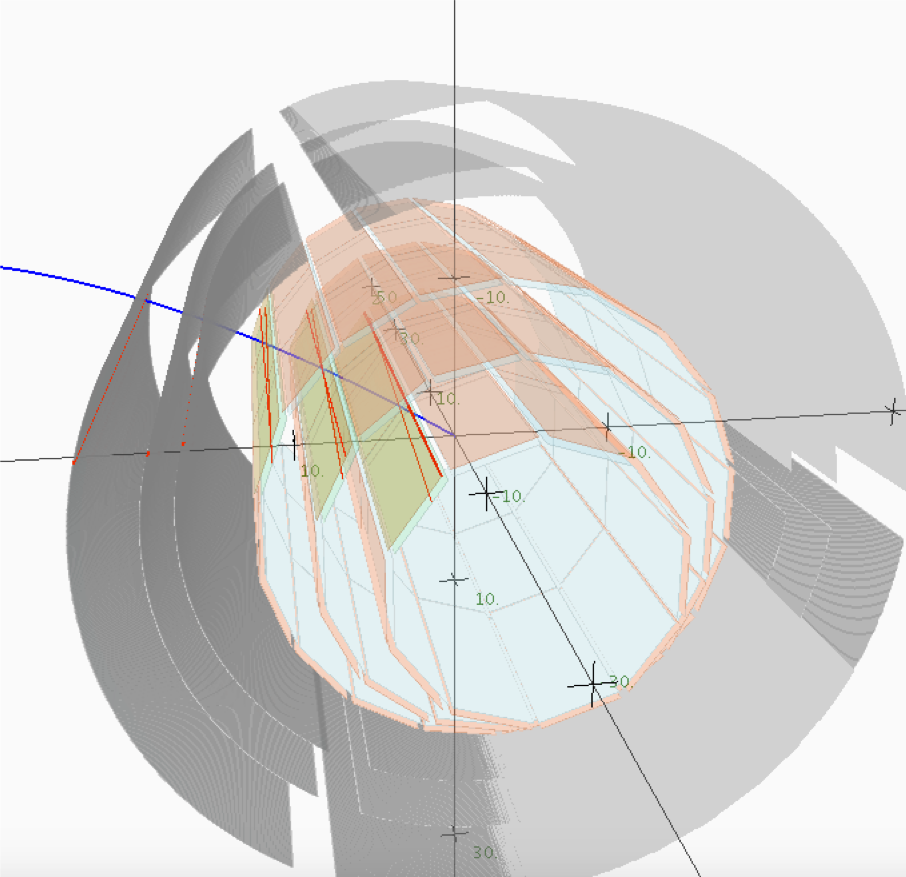
\includegraphics[width=0.5\textwidth]{pics/cvt.png}
\caption{Event display of the CVT detector. The red lines represent active SVT strips corresponding to hits on track. 
}
\label{fig:cvt}
\end{figure}

\subsubsection{Hit Clustering}
The first step of the tracking algorithm is the formation of clusters from the raw hits. The SVT raw 3-bit ADC values
are transformed into deposited charge by randomly sampling a Landau distribution fitted on test-bench data. A cluster
is a collection of contiguous hit strips. Its centroid is either given by a spatial information (a z-coordinate for
BMTC, xy-coordinates for BMTZ) or an averaged strip number for SVT. This centroid is derived by performing an average of
the relevant strip information, weighted by the maximum of the ADC pulse for micromegas strips or the equivalent
deposited charge for the SVT.
The time information associated to each hit is not used at the moment.

Before feeding all the CVT clusters to a pattern recognition algorithm, spatial coordinates must be associated to the
SVT clusters. As described in~\cite{svt-nim}, SVT layers are mechanically paired and consequently form three regions.
The readout strips of the inner and outer layer of each region make a $3^\circ$-stereo angle. By associating one
cluster of the inner layer with one cluster of the outer layer, and by assuming that an infinite momentum track crossed
perpendicularly the two layers, a preliminary candidate of the xyz-coordinates of the particle between the two layers
is derived for this cluster pair. This pairing is performed over all clusters of inner layer with all clusters of the
outer layer. Pairs whose xyz-coordinates lives outside of the SVT sensor are automatically removed from the list of
xyz-candidate list. If one of the two layer of a region has not seen the particle, then the information of the active
layer is simply ignored for the remaining of the reconstruction process.

\subsubsection{Pattern Recognition}
The trajectory of a charged particle in a solenoidal magnetic field is an helix. Because BMT detectors offers either
xy- or z-coordinates but never both, the pattern recognition cannot be performed in 3 dimensions. For particles of
large enough momentum ($p_\perp \gtrsim 0.25$ GeV/c for a 5T-solenoidal magnetic field), the xy-projection of an
helix is a circle, and the $rz$-projection is a straight line (where $r = \sqrt{x^2 + y^2}$). Therefore, a first
pattern recongition algorithm is run in xy-plane to look for circles and then a second pattern recognition algorithm is
run in rz-plane to search for straight lines.

The two pattern recognition algorithms are a modified version of the cellular automaton (CA) algorithm developed by the
Hera-B collaboration~\cite{CA-HeraB}. Here, the elementary cell of the CA is defined as a segment that connects two
2D-points.
In the $(x,y)$ plane, cells are formed with SVT and BMTZ xy-information. Two xy-clusters form a cell if the angular
distance between them is lower than a threshold. This threshold has been derived by maximizing the reconstruction
efficiency on a single track Monte-Carlo simulation with background extracted from the data. Two clusters cannot form a
cell if they are separated by more than one layer. Finally,The CA is run sector-by-sector in the BMT and, as a
consequence, a cell cannot be formed with two clusters living in different BMT sectors.
The subsequent step is the neighbor finding. A cell ``a'' is neighbor of a cell ``b'' if they share one cluster and if
the layer numbers in ``b'' are higher than the ones in ``a''. Tuned on single-track Monte-Carlo simulation without
background, cuts on the dot product between the cell directions are applied  as neighbor-forming criteria.
Now that the neighborhood of a cell is defined, the CA is evolved over $N$-evolution stage: For evolution stage $n$,
the state of all cells is updated according to $S_n = max(S_{n-1}^j) + 1$, where $S_{n-1}^j$ is the state of the
j$^{th}$-neighbor of the considered cell at evolution time $n-1$. Therefore, at evolution stage $N$, the cells with the
highest state are outer than the cells with a smalle state.
\color{red} \textbf{Caption of a figure to be produced to explain CA evolution} \color{black}

Track candidates in the $(x,y)$ plane are then formed starting from the highest state cells and following the neighbor
chain with $\Delta S = 1$. In case of multiple neighboring cells with the same state, the one that has the lower dot
product with the original cell is chosen.

Due to the poor $z$-resolution of the preliminary SVT 3D-points, the search for candidates in the $(z,r)$ plane is
performed by only using
the z-clusters of BMT. The CA algorithm trivially returns the track segments of two or three BMTC clusters.
Due to the orthogonality of the BMTC and BMTZ, all the $(z,r)$ segments of a BMT sector are combined with the $(x,y)$
candidates in the same sector. A line is fitted on the BMTC hits and its intersections with the three SVT regions are
computed. If the distance between the expected intersection and the preliminary 3D-point in the SVT region is greater
than two millimeters, then the two SVT clusters forming this preliminary point are removed from the track candidate.

\subsubsection{Track Fitting}

Each track candidate is then passed to a Kalman filter. The state vector to describe an helix is formed by five
parameters $(\varphi_0, d_0, \kappa, z_0, tan(\theta_{dip}))$, where:
\begin{itemize}
\item $d_0$ is the $(x,y)$ distance of closest approach to the CVT revolution axis,
\item $\varphi_0 = atan(p_y/p_x)$ at closest approach the the CVT revolution axis,
\item $\kappa=Q/p_\perp$ and $Q$ is the electric charge and $p_\perp=\sqrt{p_x^2+p_y^2}$,
\item $z_0$ is the distance along the $z$ axis to the CVT center,
\item and $\theta_{dip}$ is the polar angle between the track and the xy-plane.
\end{itemize}

To initialize the Kalman Filter, a first estimate of these parameters are obtained from:
\begin{itemize}
\item a circle fit in the xy-plane with SVT preliminary 3D-points and BMT xy-clusters for $d_0$, $\varphi_0$ and
$\kappa$. To improve the initialization of the fit, the point (0,0) is included in the fit with an accuracy of 100~$\mu
m$.
\item a line fit in rz-plane using only z-clusters of Micromegas to initialize $z_0$ and $\theta_{dip}$.
\end{itemize}
The covariance matrix of the two fits are merged into a 5$\times$5 matrix to initialize the covariance matrix for the
Kalman filter. Following transport equations in~\ref{ILC-Tracking}, the state vector is propagated from the CVT
revolution axis to the most outer layer of CVT, filtering at each measurement composing the track candidate. Once the
last measurement is reached, state vector and covariance matrix are brought back to the CVT revolution axis as they are
and the transport/filtering process is re-run. A maximum of five iterations is performed to make sure of the
convergence of the filtering process.

\subsubsection{Tracking Performance}

The momentum resolutions in the central and forward trackers as a function of the momentum reach
in these detectors is shown in Figs.~\ref{fig:respcvt} and~\ref{fig:respdc}, respectively.  The distributions are fit with a function of the form $\sqrt{a+b x^{2}+c/(1+d/x^{2})}$.  The resolutions achieved are well within specs and the difference in magnitude between the central and the forward trackers is due to intrinsic resolutions of these detectors.  For the forward detector, the momentum resolution in the DC is evaluated using  tracks simulated at $\theta =15\pm 5$ deg, and at $\phi = 0 \pm 5$ GeV (sample 1), to ensure that most tracks are within the sensitive volume.
Furthermore, the DC momentum resolution is correlated to the polar angle since the tracks' curvature is determined from the magnetic field intensity that is higher at lower angles in the torus field, as can be seen from Fig.~\ref{fig:restheta}, corresponding to tracks simulated at $p=4\pm 1$ GeV, $10\leq \theta\leq 25$ and $\phi = 0 \pm 5$ deg(sample 2).

These resolutions are obtained from a MC sample that does not include out of time backgrounds nor misalignments of the tracking volumes.   
A dedicated study that involves merging random background date with low luminosity data is described in [overview paper].

\begin{figure}
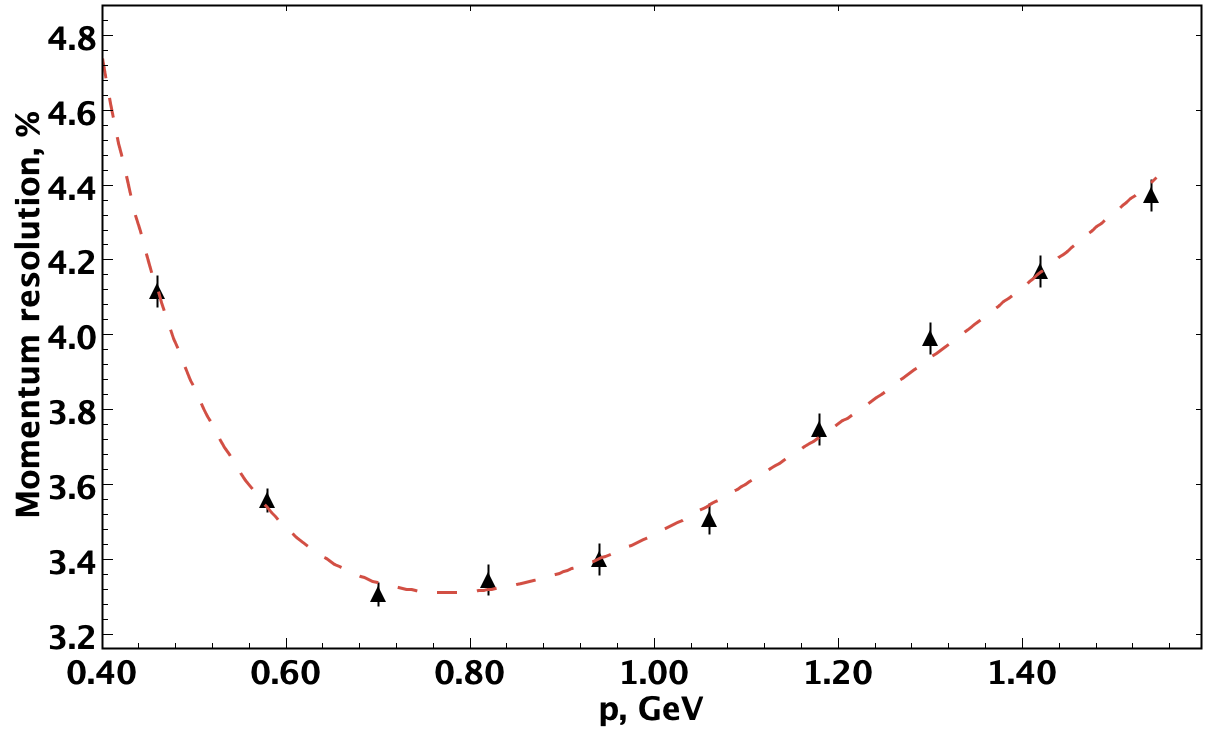
\includegraphics[width=0.45\textwidth]{pics/fddegipekmpjjiho.png}
\caption{Momentum resolution of simulated protons in the CVT.  
}
\label{fig:respcvt}
\end{figure}
\begin{figure}
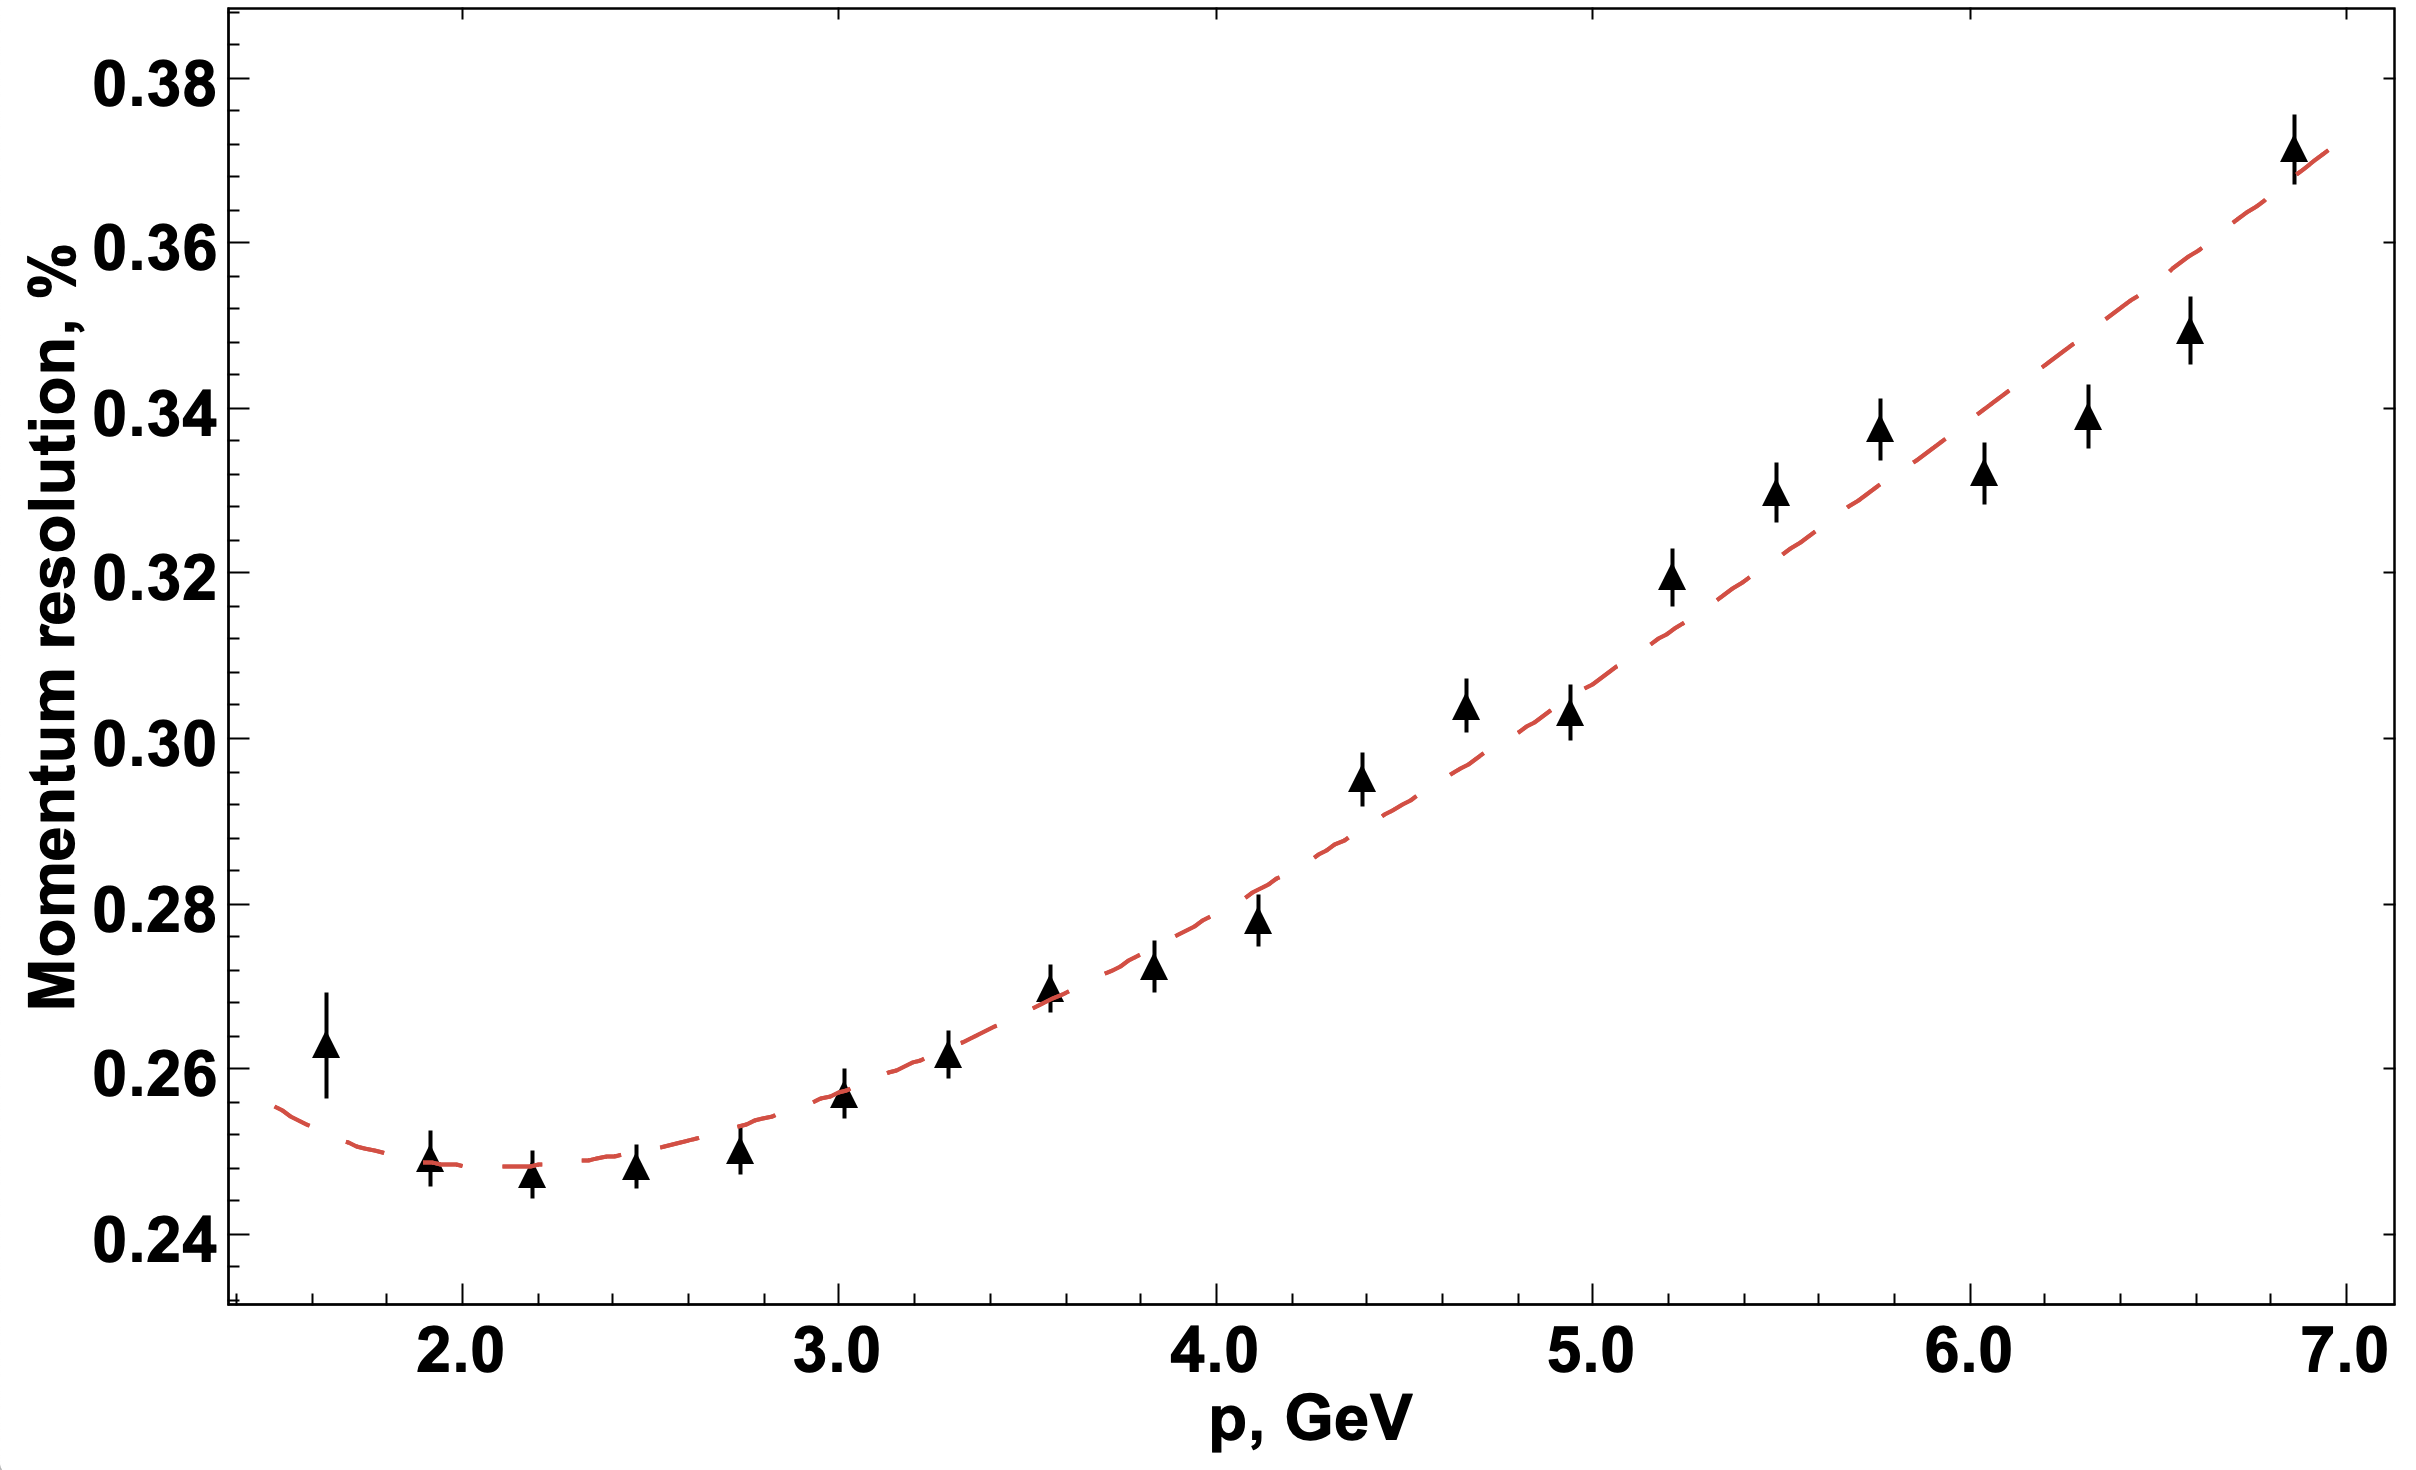
\includegraphics[width=0.45\textwidth]{pics/DCRes.png}
\caption{Momentum resolution in the DC evaluated using pions  simulated at $\theta =15\pm 5$ deg, and at $\phi = 0 \pm 5$ deg.
}
\label{fig:respdc}
\end{figure}

\begin{figure}
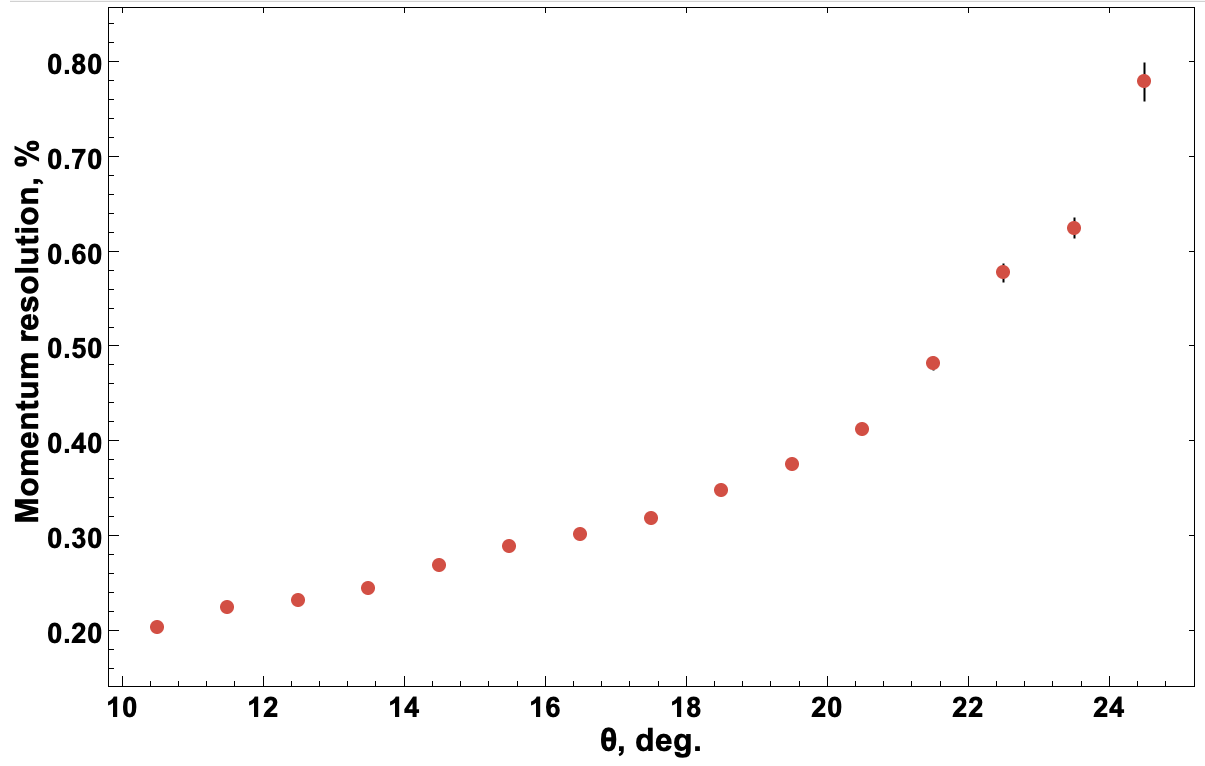
\includegraphics[width=0.45\textwidth]{pics/DCRes2.png}
\caption{Momentum resolution in the DC evaluated using  pions  simulated at $p=4\pm 1$ GeV, $10<\leq \theta\leq 25$ and $\phi = 0 \pm 5$ deg.
}
\label{fig:restheta}
\end{figure}

The tracking efficiency for in- and out-bending tracks calculated from sample 1 is shown in  Figs.~\ref{fig:trkeff}.  In-bending tracks suffer from a loss in tracking efficiency for momenta generated below 1.8 GeV at time-base level due to lack of matching with the outer detectors.  These tracks miss the sensitive volumes of the Time-of-Flight system which is required to extract time correction information needed for time-based tracking.  They do however pass the hit-base requirement.  The efficiency loss due to the afore mentioned effect can be seen by comparing the (light) blue distribution to the (dark) red one.  In the momentum range from 1.8 to 7.5 GeV, the time-based tracking efficiency is 98\%, while in the range from 1.4 to 7.5 GeV, the hit-based tracking efficiency is 99\%.  For out-bending tracks (Fig.~\ref{fig:trkeff}(bottom)), both the hit-based and time-based tracking efficiencies are flat as a function of momentum and of the order of 99\%. 


\begin{figure}
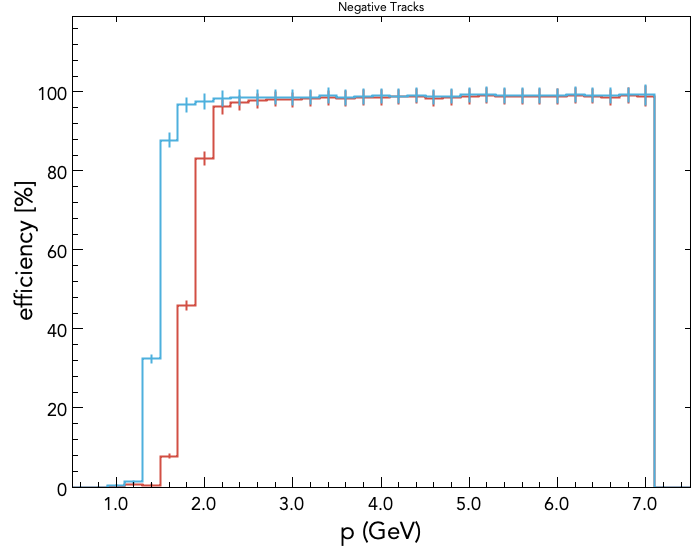
\includegraphics[width=0.45\textwidth]{pics/DCTrkgEffNegTrks.png}
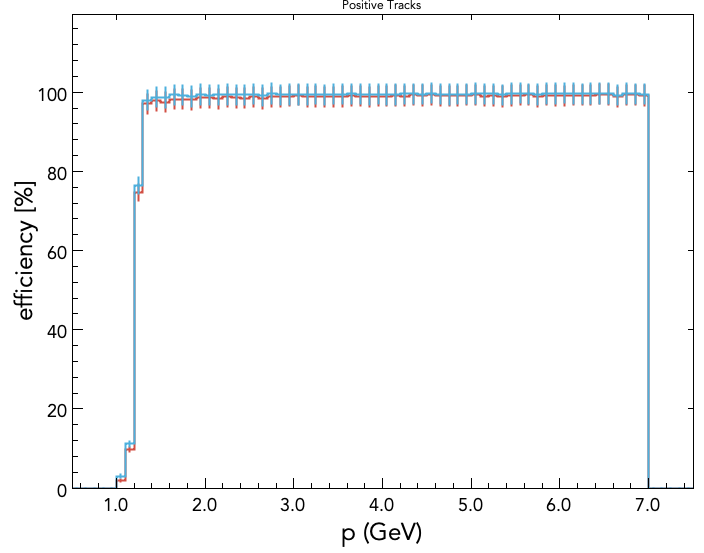
\includegraphics[width=0.45\textwidth]{pics/DCTrkgEffPosTrks.png}
\caption{DC tracking efficiency as a function of momentum evaluated using  (top) negative and (bottom) positive pions simulated at $\theta =15\pm 5$ deg, and at $\phi = 0 \pm 5$ deg. The (light) blue and (dark) red distributions correspond to the hit- and time-based tracking efficiencies, respectively.
}
\label{fig:trkeff}
\end{figure}


The polar angular dependence of the tracking efficiency obtained from sample 2 is shown in Fig.~\ref{fig:trkeffinoutb}.   The (light) green spectrum corresponds to out-bending tracks.  The efficiency is flat in the angular range from 10 to 25 deg. for outbending tracks while there is a loss of tracks below 15 deg.  As before, this is due to tracks missing the outer detectors.  

\begin{figure}
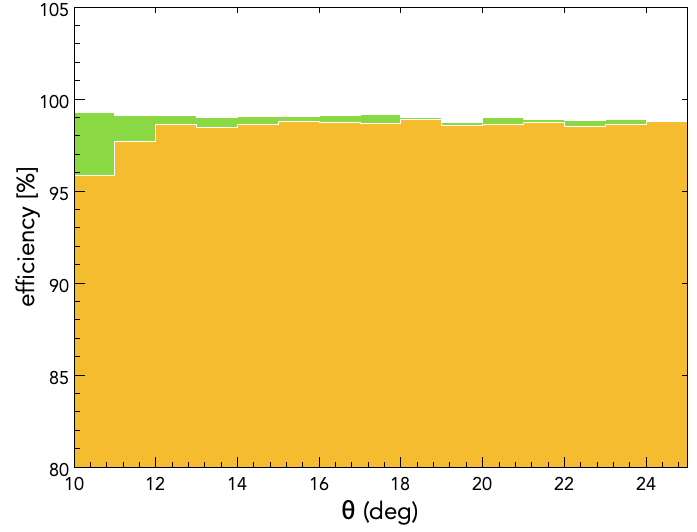
\includegraphics[width=0.45\textwidth]{pics/DCTrkEffvsThetaInandOutbenders.png}
\caption{DC tracking efficiency as a function of polar angle evaluated using  pions  simulated at $p=4\pm 1$ GeV, $10\leq \theta\leq 25$ and $\phi = 0 \pm 5$ deg.
}
\label{fig:trkeffinoutb}
\end{figure}

\subsection{Electromagnetic Calorimeters}

The Electromagnetic Calorimeters (ECAL)~\cite{ecal-nim} of the CLAS12 Forward Detector downstream of the
torus and the FTOF are lead-scintillator strip sampling calorimeters used for the detection of electrons, photons,
and neutrons. A pre-shower calorimeter (PCAL) is positioned in front of the EC calorimeter, which consists of two
parts, EC-inner (ECIN) and EC-outer (ECOU). The ECAL reconstruction service provides a fast
and efficient algorithm for grouping scintillator {\it strips} with {\it hits} into multiple {\it peaks} and {\it clusters}
within the three submodules, PCAL, ECIN, and ECOU, for each of the six ECAL modules, while leaving cluster
matching and particle identification to the Event Builder service.

Within the ECAL reconstruction service, these various elements exist as objects with methods, structures, and data
members designed for calibration, pattern recognition, diagnostics, and serial output. For example, the service applies
run-dependent calibration corrections for conversion of the raw ADC and TDC digitized data to energy and time, and
also provides formatted output banks used by external services.  Energy thresholds and cluster identification criteria
can also be configured to optimize the reconstruction efficiency, suppress backgrounds, and avoid false or duplicate
clusters arising from fluctuations at the fringes of the electromagnetic showers.

The cluster finding algorithm makes use of the unique geometry and stereo readout features of the ECAL. As
discussed in Ref.~\cite{ecal-nim}, each triangular scintillator layer in the ECAL lead:scintillator sandwich is
transversely divided into strips, with the shortest strip at the corners. The slice direction rotates by 120$^\circ$
for each successive layer, providing three {\it views} labeled $U$, $V$, and $W$.  For each strip within a view,
layers are optically ganged together into a stack.  Individual photomultiplier tube (PMT) readout of each PCAL,
ECIN, and ECOU stack provides a pulse proportional to the summed energy deposited in the stack.

The algorithm begins by finding collections of contiguous stacks having signals above a user-defined threshold for
each of the three views. These groupings are called {\it peaks} and their member stacks are referred to as
{\it hits}.  Peak objects may be further subdivided based on the hit energy profile of the groupings. Each peak
object is associated with one or more stacks of strips that belong to it, and the three-dimensional geometry of each
stack is stored along with the peak data. The service uses this geometry data to determine which collection of
peaks belong to {\it clusters}.

\subsubsection {Cluster Position}
\label{ec-cluster}

The criterion for defining a cluster requires the spatial intersection of three peaks, one from each of the $U$,
$V$, and $W$ views. Candidate peaks for a cluster search are based on a user-defined threshold for the
summed peak raw energy. Each peak is represented geometrically as a directed line segment determined by the
energy-weighted average of the mid-lines of each member strip. The degree of intersection of each $U$, $V$,
and $W$ peak triplet is determined by calculating the line of closest distance between a $U$ and $V$ peakline,
followed by the line of closest distance between the midpoint of the $UV$ line and the $W$ peakline. A
user-defined cut on this final $UV$-$W$ distance identifies the cluster, and the midpoint of the $UV$-$W$
line defines the transverse $(x',y')$ coordinates of the cluster in the local coordinate frame (with the $z'$
axis perpendicular to the ECAL planes). The longitudinal coordinate $z'$ is set to coincide with the layer of
maximum energy deposition to minimize parallax effects for tracks that are not perpendicular to the detector
surface~\cite{ecal-nim}. As the cluster reconstruction is performed before the matching with the other CLAS12
detectors that can provide particle identification, the same algorithm is applied to clusters originating from
charged or neutral particles.

\subsubsection {Cluster Energy}

Once the cluster is localized, the path from the cluster position to the PMT readout end is calculated for each $U$,
$V$, $W$ peakline and the peak energies are corrected for scintillator light attenuation. For isolated clusters,
the cluster energy is then defined as the sum of the corrected energy from each of the $U$, $V$, and $W$ peaks
that define the cluster.

More complicated scenarios arise from the triangular geometry of the ECAL hodoscope, which creates the
possibility of a single peak in the $U$, $V$, or $W$ view that shares the summed energy from two or more
clusters. For these cases, the energy in each cluster that shares that peak is assumed to be proportional to the
relative partial energies of the multiple clusters as measured in the other views. For example, if there are two
clusters, both of which share the same $U$ peak, the summed energy $V+W$ is determined for each of the
clusters, and the ratio of these summed energies determines how much of the $U$ peak energy is assigned to
each of the two clusters.

Finally, the clusters to be reported to external services are selected with a user-defined energy cut, and these
clusters are sorted according to energy. Typical software thresholds applied at the stacks, peak, and cluster level
are 1, 3, and 10~MeV, respectively.

\subsubsection {Cluster Time}
\label{ec-time}

Once the cluster is localized, the path from the cluster position to the PMT readout end is calculated for each
$U$, $V$, $W$ peakline and the peak timing is corrected for the propagation delay of the light, using the effective
velocity of light determined for each scintillator from the calibration procedure. For isolated clusters, the cluster
timing is then taken from the $U$, $V$, or $W$ peak with the largest uncorrected raw ADC value. This minimizes
the effect on the timing resolution from both the time-walk correction (i.e. the signal amplitude dependence of the
hit time) and the photoelectron statistical fluctuations.

\subsection{Threshold Cherenkov Counters}

The CLAS12 Forward Detector includes two threshold Cherenkov detectors for particle identification. The
High Threshold Cherenkov Counter (HTCC)~\cite{htcc-nim} is located upstream of the torus and is used for
identification of the scattered electron in conjunction with the ECAL. The Low Threshold Cherenkov Counter
(LTCC)~\cite{ltcc-nim} is positioned upstream of the FTOF and is used mainly to separate pions from kaons.
Both the HTCC and LTCC are large gas-filled volumes (CO$_2$ for the HTCC, C$_4$F$_{10}$ for the LTCC)
with mirrors that direct light collection to the PMTs. The goal of the HTCC and LTCC reconstruction algorithms
is to calculate the signal strength, time, and position from the raw ADC signals (read out with flash ADC boards
- FADCs). The algorithm takes into account the properties of the HTCC and LTCC geometries, namely, the
possibility for the signal from the single track to split into up to four mirrors. Hence, up to four separate
signals (or hits) are produced. The final signal reconstruction is done in three steps: decoding, hit reconstruction,
and cluster reconstruction. For each hit, the signal strength ($nphe_{hit}$ - the number of photoelectrons) is
determined from the pedestal-subtracted integral of the FADC pulse and the associated time ($T_{hit}$) is
determined from a fit of the position of the FADC signal threshold crossing time.

At the hit reconstruction stage, individual signals in terms of the ADC channels are converted into the number of
photoelectrons ($nphe_{hit}$) for each hit using gain constants derived from the detector calibration and stored
in CCDB:

\begin{equation}
nphe_{hit} = \frac{ADC}{gain}.
\end{equation}

\noindent
Geometry information on the PMT location is used to associate the angular coordinates ($\theta_{hit}$, $\phi_{hit}$)
to the hit.

In order to reconstruct the real signal strength ($nphe_c$), split signals (hits) have to be combined into a single
cluster. The algorithm starts by selecting the hit with the largest $nphe_{hit}$, which is used as a seed for the
cluster. Adjacent hits within a certain time window are then searched iteratively and, if found, added to the
cluster. The total signal strength is determined as the sum of the individual signals, and the signal time is
determined as the average between the individual signal times, weighted by the corresponding number of
photoelectrons. The cluster angular coordinates are determined as the average between the individual hits forming
the cluster. The cluster quantities are defined by:

\begin{eqnarray}
nphe_c &= \frac{\sum_{i=1}^N{nphe_{hit}}}{N} \nonumber \\
T_c &= \frac{\sum_{i=1}^N{N*T_{hit}}}{\sum_{i=1}^N{nphe_{hit}}} \nonumber \\
\theta_c &=\frac{\sum_{i=1}^N{\theta_{hit}}}{N} \nonumber \\
\phi_c &= \frac{\sum_{i=1}^N{\phi_{hit}}}{N}.
\end{eqnarray}

\noindent
The clustering algorithm is run iteratively until the full list of $N$ hits is exhausted.

In the HTCC, the cluster coordinates, required for the matching of the hit with the reconstructed track in the
Event Builder, are reconstructed by projecting  ($\theta_c$, $\phi_c$) of the cluster on the surface of the
ellipsoidal mirror of the detector. In the LTCC, an estimated cluster position is calculated based on a
parameterization extracted from Monte Carlo simulations. The track that passes the closest to the cluster
position is then chosen as the match for this cluster.

\subsection{Ring-Imaging Cherenkov (RICH)}

One of the six CLAS12 Forward Carriage sectors has been equipped with a Ring Imaging Cherenkov detector \cite{rich-nim}.

\subsubsection{Geometry}
The RICH mirror geometry is implemented through both of the native GEMC geometry API and imports from the engineering model STEP files.
The spherical mirrors are made through Geant4 boolean intersections of spheres and planes.
Since the array of 391 PMTs is inside the CLAS12 acceptance, particular care went into implementing in the
simulation the details of the PMT hardware and materials: the PMTs are Geant4 aluminum boxes containing the electronics components
(including the adapter, ASIC and FPGA boards), the window, the photocathodes.
Each PMTs contain 64 pixel. The identification of the pixel is done in the process identification routine.
The aerogel are Geant4 boxes.
The RICH box, mirror support structure, and additional support hardware are imported directly from the engineering CAD models.
\F{richGeometry} shows details of the geometry implementation.

\begin{figure}
	\centering
	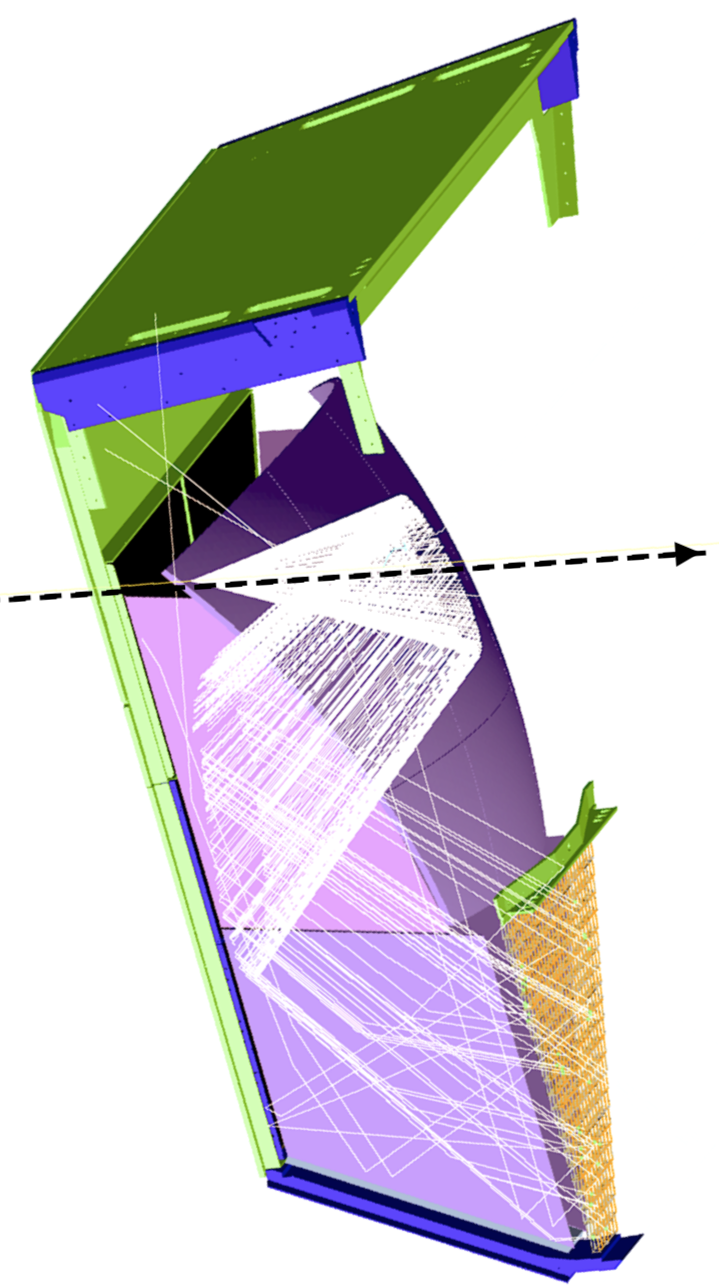
\includegraphics[width=0.99\columnwidth, keepaspectratio]{img/richGeometry.png}
	\caption{The implementation of the RICH geometry. Beam is incident from the left. A 4 GeV kaon produces a Cherenkov light cone.
			 Part of the cone reflects onto the spherical mirror and into the PMT array. The remaining photons go through the aerogel tiles
			 and bounce off the planar mirror onto the PMT array. All inefficiencies are taken into account by using the aerogel refractive index
			 and its transparency. }
	\label{fig:richGeometry}
\end{figure}

The refractive index of the aerogel and its transparency is included in the material optical properties and taken
into account during the Geant4 transportation of the photons.
Similarly for the reflectivity of the mirrors. The quantum efficiency associated with the PMT photocathodes is taken into account in the digitization routine.

\subsubsection{Process ID}
At each Geant4 step, the local coordinates in the PMT volume are used to calculate the pixel number within that PMT.

\subsubsection{Digitization}

Photons that impinge on the PMT faces are processed with the digitization routine.
Each photon collected is input to the quantum efficiency algorithm at its wavelength to decide if it is detected.
The ADC energy is calculated and smeared using the single photo-electron peak position and width from the calibration database.
The time average of all the photons is saved in the output.
The digitized output bank variables are summarized in Table \ref{tab:richBank}.

\begin{table}[h]
	\begin{center}
		\begin{tabular}{| c | c | c |}
			\hline \hline
			Variable & Description                                         \\
			\hline
             sector  &                                     CLAS12 sector   \\
                pmt  &                                        PMT number   \\
              pixel  &                       pixel number within the PMT   \\
                ADC  &                                               ADC   \\
               time  &                           average time of the hit   \\
               nphe  &                  number of photoelectrons arrived   \\
              npheD  &                 number of photoelectrons detected   \\
               hitn  &                                        hit number   \\
			\hline \hline
		\end{tabular}
	\end{center}
	\caption{The digitized RICH bank.}\label{tab:richBank}
\end{table}

The time window  of the RICH is set to 5 ns: all Geant4 steps within the same PMT pixel and time window are collected in one hit.

\subsection{Time-of-Flight Systems}
\label{tof-sys}

The time-of-flight (TOF) detectors for CLAS12 include the Forward Time-of-Flight system (FTOF)~\cite{ftof-nim}
and Central Time-of-Flight system (CTOF)~\cite{ctof-nim}. The FTOF consists of planes of scintillator counters
located between the RICH/LTCC and the ECAL. Two parallel counter arrays in each Forward Detector sector are
employed to achieve the desired time resolution in the polar angle range from 5$^\circ$ to 35$^\circ$. The arrays are
referred to as panel-1b (closer to the target) and panel-1a (farther from the target). A third set of counter arrays
referred to a panel-2 covers polar angles from 35$^\circ$ to 45$^\circ$. The different FTOF arrays can be seen in
Fig.~\ref{fig:dcTracks}. The CTOF consists of a barrel of scintillator counters located just outside of the CVT within
the solenoid.

The raw data from the detector PMTs read out during data acquisition include an ADC charge and hit time from a
fitted flash ADC (FADC) waveform and a TDC time. The ADC and TDC information is read out and recorded only for
those channels that are above the $\sim$1~MeV hardware readout threshold for the FADCs and discriminators of
both systems. 

As the FTOF and CTOF counters employ double-ended PMT readout, the calibration procedures for these
systems (described in detail in Refs.~\cite{ftof-nim,ctof-nim}) allow the reconstruction to report accurate hit
times and deposited energy associated with both PMT signals above threshold. At this point the event reconstruction
combines the PMT hit times and energies to give a hit time and energy deposition associated with the scintillation
counter. In a second phase, hits in adjacent counters, due to particles that pass through multiple counters in the
FTOF and CTOF systems (so-called ``corner clippers''), are combined into clusters with an associated time,
coordinate, and deposited energy. The algorithms for the hit and cluster definitions are detailed in the next sections.

\subsubsection{Raw Counter Hits}

Raw hits for the TOF systems are defined by matching the ADC and TDC information reported for each counter. This
matching is based on the comparison of the TDC time with the time from the FADC waveform analysis. The latter is
derived from fitting the leading edge of the FADC pulse shape during data decoding. Due to the choice of fast timing
PMTs for the detector readout and the use of 250~MHz FADCs, the number of samples on the leading edge of the
PMT pulses is only 3 to 4, hence the FADC timing resolution is only $\sim$1~ns. The FADC and TDC times are then
required to be within a selected window. The windows parameters, position, and width, as well as all other constants
used by the reconstruction package, are loaded at run time from CCDB. Currently the window width used is 10~ns,
which was found to be sufficient to reduce the probability of a mismatch of the ADC and TDC data for a given
scintillation bar hit. This is especially important for the FTOF as the ADC value of the hit is used to compute the
time-walk correction.

\subsubsection{Reconstructed Counter Hits}
\label{rec:hits}

Raw hits are processed to determine reconstructed hits with energy, time, and position information.  The
reconstructed hit times from the individual PMTs need to account for the time delays along the readout path
that include the PMT signal transit time, the signal propagation times through the signal cables and the electronics,
and any time-walk effects associated with the readout discriminators. For the FTOF readout, leading-edge
discriminators are employed, while for the CTOF readout, constant fraction discriminators are employed and no
external time-walk corrections are required. The hit times reconstructed by the TDC readout of the PMTs at the
ends of each scintillation bar (referred to generically here as 1 and 2) are given by:

\begin{multline}
t_{1/2} = (CONV \cdot TDC_{1/2}) - t_{1/2}^{walk} \\ \mp \frac{C_{12}}{2} + C_{RF} + C_{p2p},
\end{multline}

\noindent
where $CONV$ is the TDC channel-to-time conversion factor (0.024~ns/bin), $TDC$ is the measured PMT TDC
value relative to the trigger signal, $t^{walk}$ is the time-walk correction that accounts for the pulse amplitude
dependence of the crossing times of the discriminator threshold (used only for FTOF), $C_{12}$ is a time offset
to center the PMT TDC difference distribution about 0, and $C_{RF}$ and $C_{p2p}$ are the time offsets to
align all of the counter hit times with respect to the accelerator RF time and to each other, respectively. The
paddle-to-paddle time offsets $C_{p2p}$ mainly account for the signal delays along the cable lengths from the PMT
output to the readout electronics.

The FTOF and CTOF particle hit times relative to the trigger signal can be determined separately from the times
$t_1$ and $t_2$ measured by the PMTs of a given scintillation bar using:

\begin{equation}
\label{thit-1}
t_{hit}^{1/2} = t_{1/2} - \frac{d_{1/2}}{v_{eff}},
\end{equation}

\noindent
where $d_{1/2}$ represents the distances along the bar from the hit point to the PMT given by:

\begin{equation}
d_{1/2}= L/2 \pm y,
\end{equation}

\noindent
with $y$ the hit coordinate along the bar (determined from forward tracking for the FTOF and central tracking
for the CTOF) and $L$ is the counter length. The average counter hit time is given by:

\begin{equation}
\label{thit-2}
\bar{t}_{hit} = \frac{1}{2} ( t_{hit}^1 + t_{hit}^2 ) = \frac{1}{2} \left[ t_1 + t_2 - \frac{L}{v_{eff}} \right],
\end{equation}

\noindent
where $v_{eff}$ is the effective speed of light in the scintillation bar.

Using the timing information from the PMTs at the ends of each bar, the hit coordinate along the bar with respect
to the center of the bar can be defined from the FTOF or CTOF information alone using:

\begin{equation}
\label{tof-coor}
y = \frac{v_{eff}}{2} (t_1 - t_2 - C_{12}).
\end{equation}

\noindent
It is this coordinate determination that is compared against the projected coordinate from tracking to determine
if the time-of-flight hit matches to a projected track.

The algorithm detailed above and currently in use requires good ADC and TDC information for the PMTs at both
ends of the counter to be available. However, if one of the PMTs of a counter is malfunctioning, Eq.(\ref{thit-1})
shows that the hit time recorded from the working PMT alone can be used to reconstruct the particle hit time using
tracking information to correct for the light propagation delay along the counter. The loss of one PMT involves a
$\sqrt{2}$ worse timing resolution for the counter. Algorithms to address these cases are already implemented in
the reconstruction service but are presently disabled.

The reconstructed energies from the ADC values of the PMTs (1 and 2) for a given scintillator bar are given by:

\begin{equation}
E_{1/2} = (ADC_{1/2} - PED_{1/2}) \left [ \frac{\left( \frac{dE}{dx} \right )_{MIP} \cdot t}{ADC_{MIP}} \right ],
\end{equation}

\noindent
where $(ADC-PED)$ is the measured pedestal-subtracted ADC integral, $ADC_{MIP}$ is the ADC value for
normally incident minimum-ionizing particles (MIPs) at the center of the scintillation bar,
$\left( \frac{dE}{dx} \right)_{MIP}$ is the energy loss for MIPs in the scintillation bars (2.001~MeV/cm), and
$t$ is the scintillation bar thickness. The deposited energy is computed as the geometric mean of the deposited
energy as determined from the two counter PMTs as:

\begin{equation}
E_{dep} = \sqrt{E_1 E_2}.
\end{equation}

\subsubsection{Hit Clustering and Matching}
\label{sec:tof-cluster}

If there are multiple scintillation bar hits associated with a single incident charged particle track, a hit cluster
can be defined. These clusters have associated with them a hit coordinate, deposited energy, and hit time. Hits
are assigned as part of a cluster in either the FTOF or CTOF if their hit positions and hit times fall within selected
matching windows. The clustering algorithm looks to define hit clusters matched to tracks separately in each of the
counter arrays.

With hit clusters defined, the associated cluster coordinate along the counter length is defined as the
energy-deposited weighted average of the reconstructed $y$ coordinate from Eq.(\ref{tof-coor}) as:

\begin{equation}
y_{cluster} = \sum_{i=1}^{N} y_i \cdot \Delta E_i.
\end{equation}

\noindent
Note that in both the FTOF and CTOF systems, the maximum cluster size is practically limited to $N=2$. For the
coordinate transverse to the counter length along the counter width, the coordinate is defined as the average of
the coordinates associated with the middle of the bar.

The assigned cluster energy is the sum of the deposited energies in the counters associated with the defined
cluster,

\begin{equation}
  E_{cluster} = \sum_{i=1}^N E_{dep}^i.
\end{equation}

In the FTOF when there is a defined hit or a defined cluster in both panel-1b and panel-1a, a second cluster matching
algorithm is applied to determine if the hit or cluster in panel-1b and the hit or cluster in panel-1a are associated with
the same incident track matched to the panel-1b hit or cluster. If they are associated, a corrected FTOF hit time based
on the panel-1a and panel-1b cluster times is computed using a time resolution weighting according to the counter in
each cluster with the largest energy deposition using:

\begin{equation}
  t_{corr} = \frac{\displaystyle \frac{\displaystyle t_{1b}^{cluster}}{\displaystyle \delta_{1b}} +
    \frac{\displaystyle (t_{1a}^{cluster} - \Delta r/\beta c)}{\displaystyle \delta_{1a}}}
  {\displaystyle \left( \frac{\displaystyle 1}{\displaystyle \delta_{1b}} +
    \frac{\displaystyle 1}{\displaystyle \delta_{1a}} \right)}.
\end{equation}

\noindent
Here $\delta_{1a,1b}$ are the effective time resolutions measured for the counters determined during the
FTOF calibration procedure and $t_{1a,1b}^{cluster}$ are the cluster hit times in panel-1a and panel-1b. The term
$\Delta r/(\beta c)$ accounts for the path length difference between the panel-1b cluster hit coordinate and
the panel-1a cluster hit coordinate and comes from forward tracking information. As $\beta$ depends on the
FTOF time, it is assumed that it is based on the panel-1b time information (the array with the better timing
resolution).

Given the effective FTOF counter resolutions, the overall FTOF hit time resolution is improved by 15-20\%
when combining the times from panel-1b and panel-1a in this manner. Of course, if the track interacts with only
panel-1a or with only panel-1b due to the slightly different solid angles of coverage of the arrays, then only the
single plane hit time is used in the event reconstruction. 

Note that employing the cluster times has not yet been fully validated in the event reconstruction but is currently
under test using Monte Carlo data samples. While this validation is in progress, the information passed from the
time-of-flight systems to the Event Builder is based on reconstructed hits.

\section{Central Neutron Detector (CND)}


The CLAS12 CND geometry is created using the native gemc geometry API.
The geometry directory is "cnd"

\subsection{Geometry}

\subsubsection{Geometry Git Location}

\subsection{Process ID}

\subsection{Digitization}

\subsubsection{Summary of CCDB Table used}

\subsection{Digitized Bank}

\subsubsection{Time Window}

\subsubsection{Process Routine Git Repository Location}



\subsection{Forward Tagger (FT)}


\subsubsection{Geometry}

The FT consists of three subsystems:

\begin{itemize}
	\item a micromegas tracker (FT-TRK);
	\item a hodoscope (FT-HODO);
 	\item a calorimeter (FT-CAL).
\end{itemize}

The three subsystems are implemented in GEMC using the native perl API script, except for the inner shield (see Section \ref{sec:beamline}),
which comes from the CAD engineering model.
The FT geometry is shown in \F{ftGeometry}.

\subsubsection{Digitization}

\begin{figure}
	\centering
	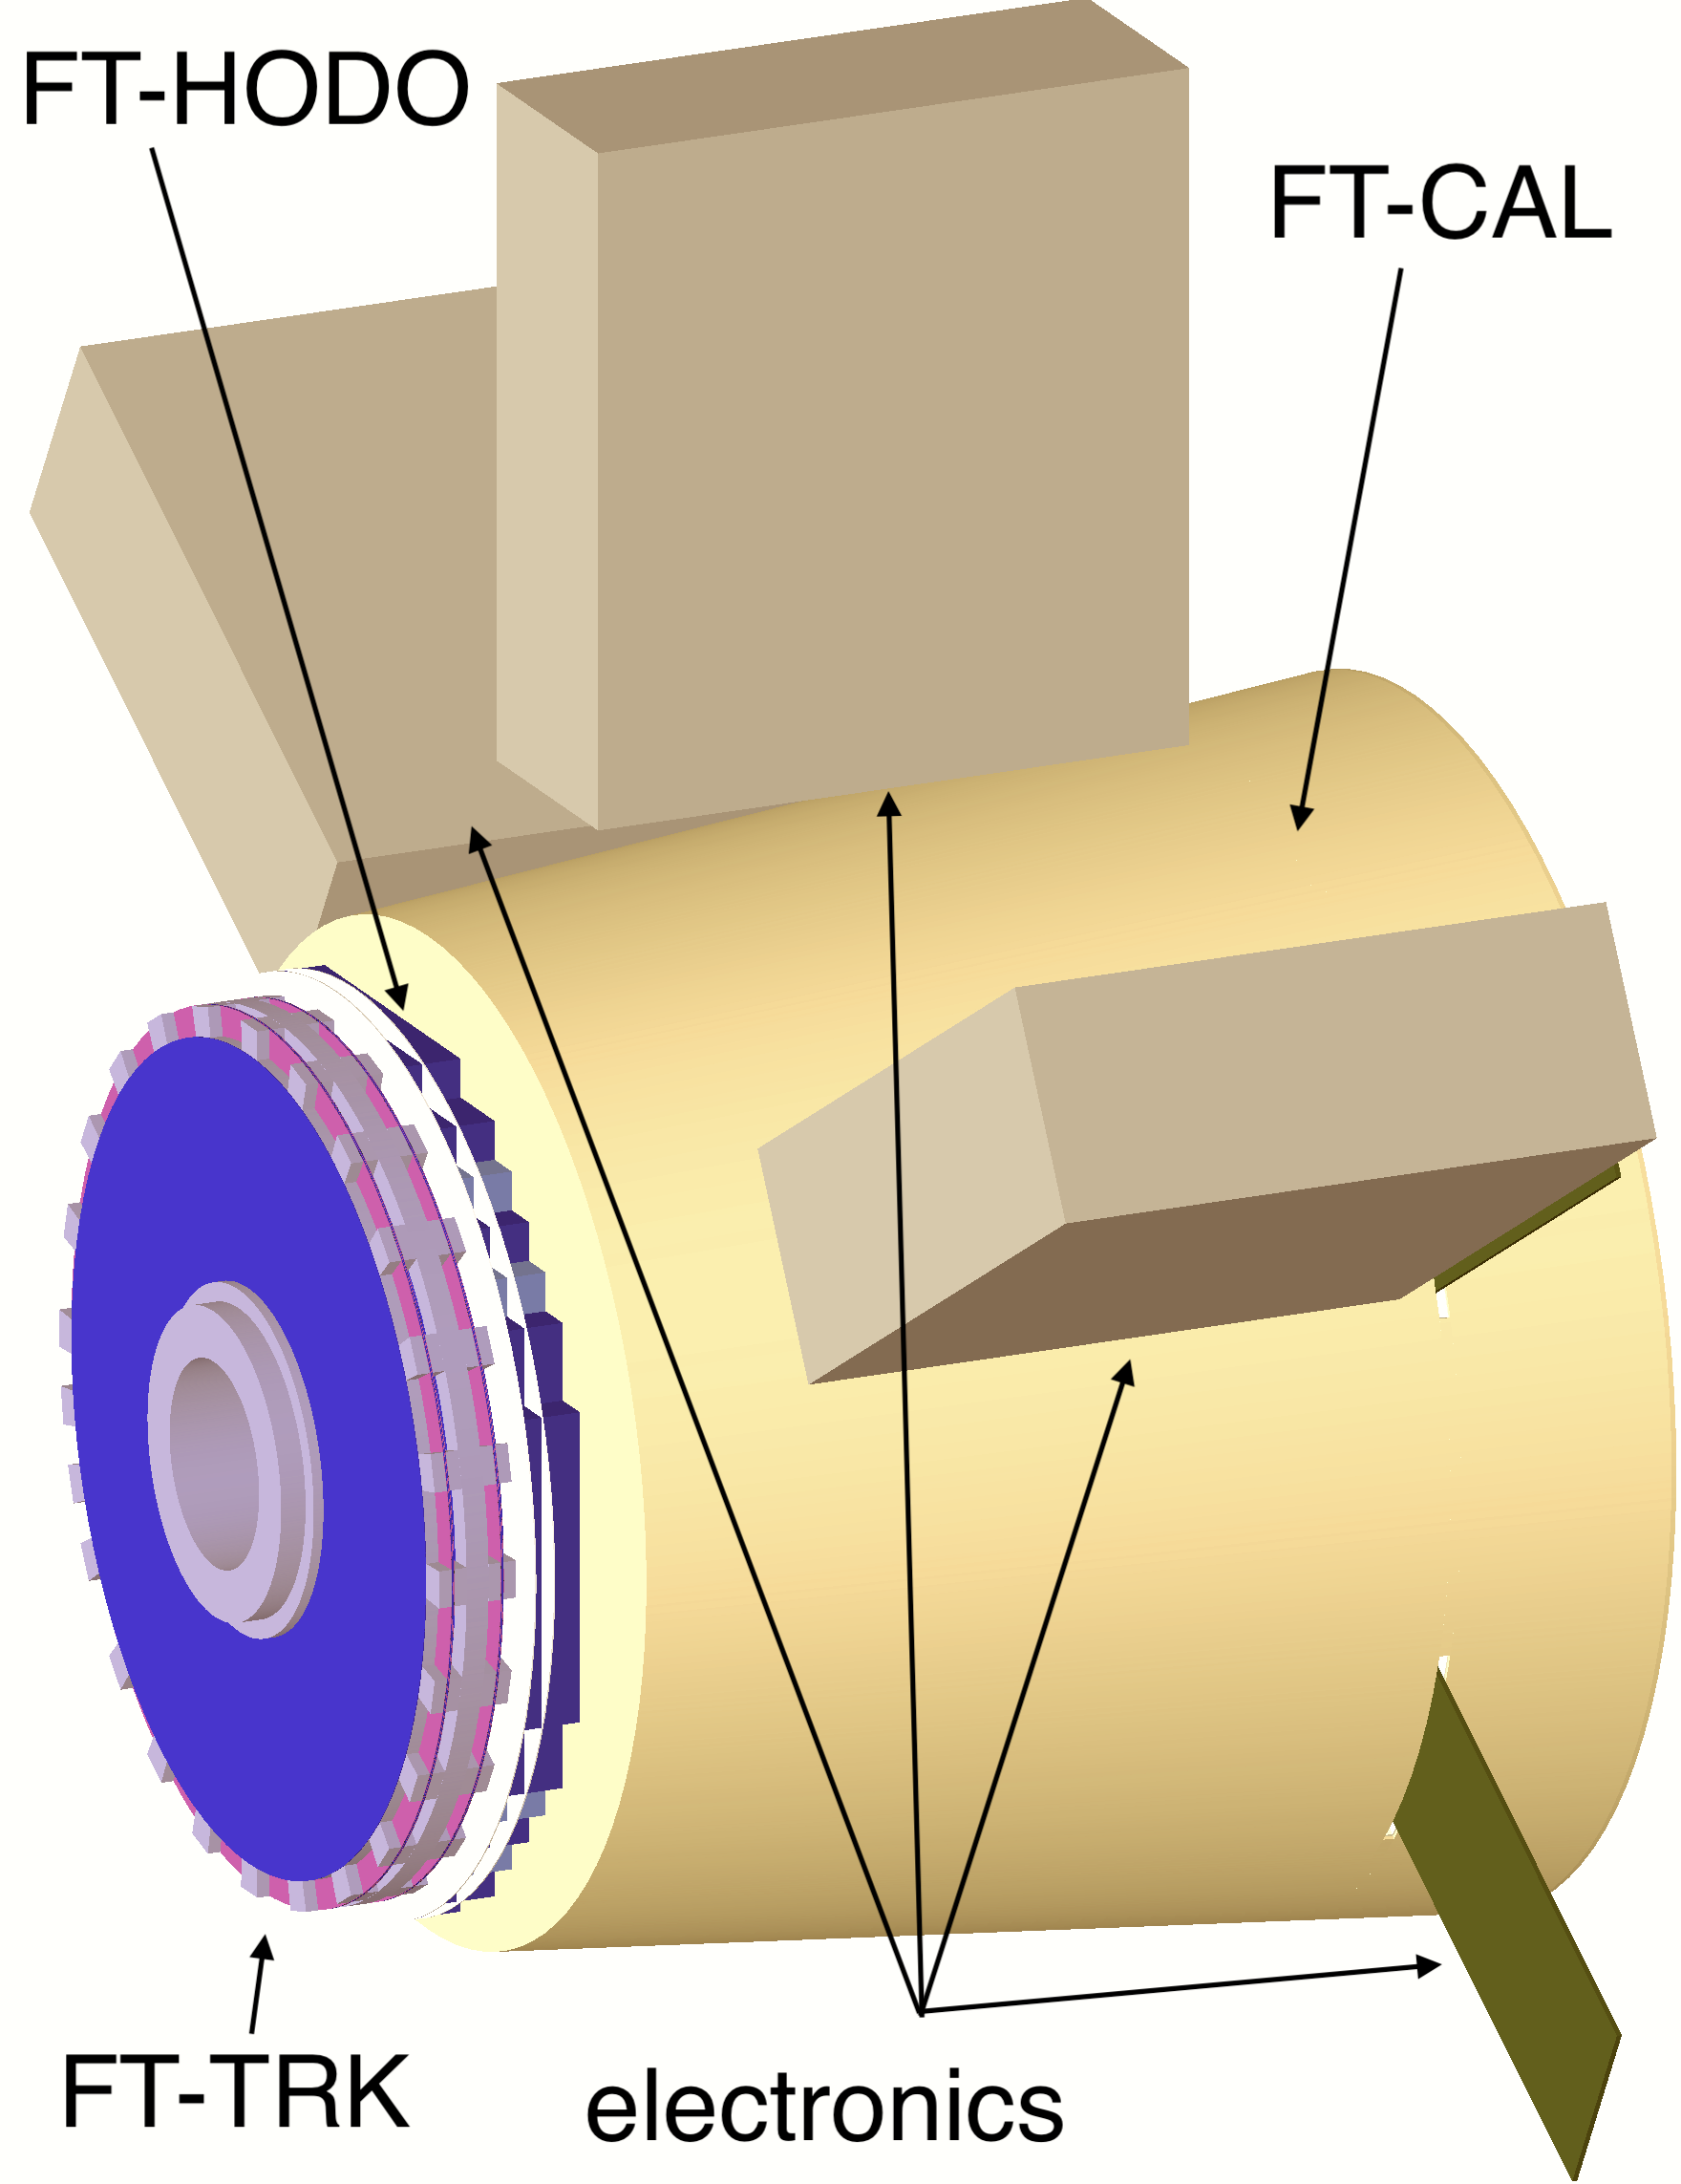
\includegraphics[width=0.99\columnwidth,keepaspectratio]{img/ftGeometry.png}
	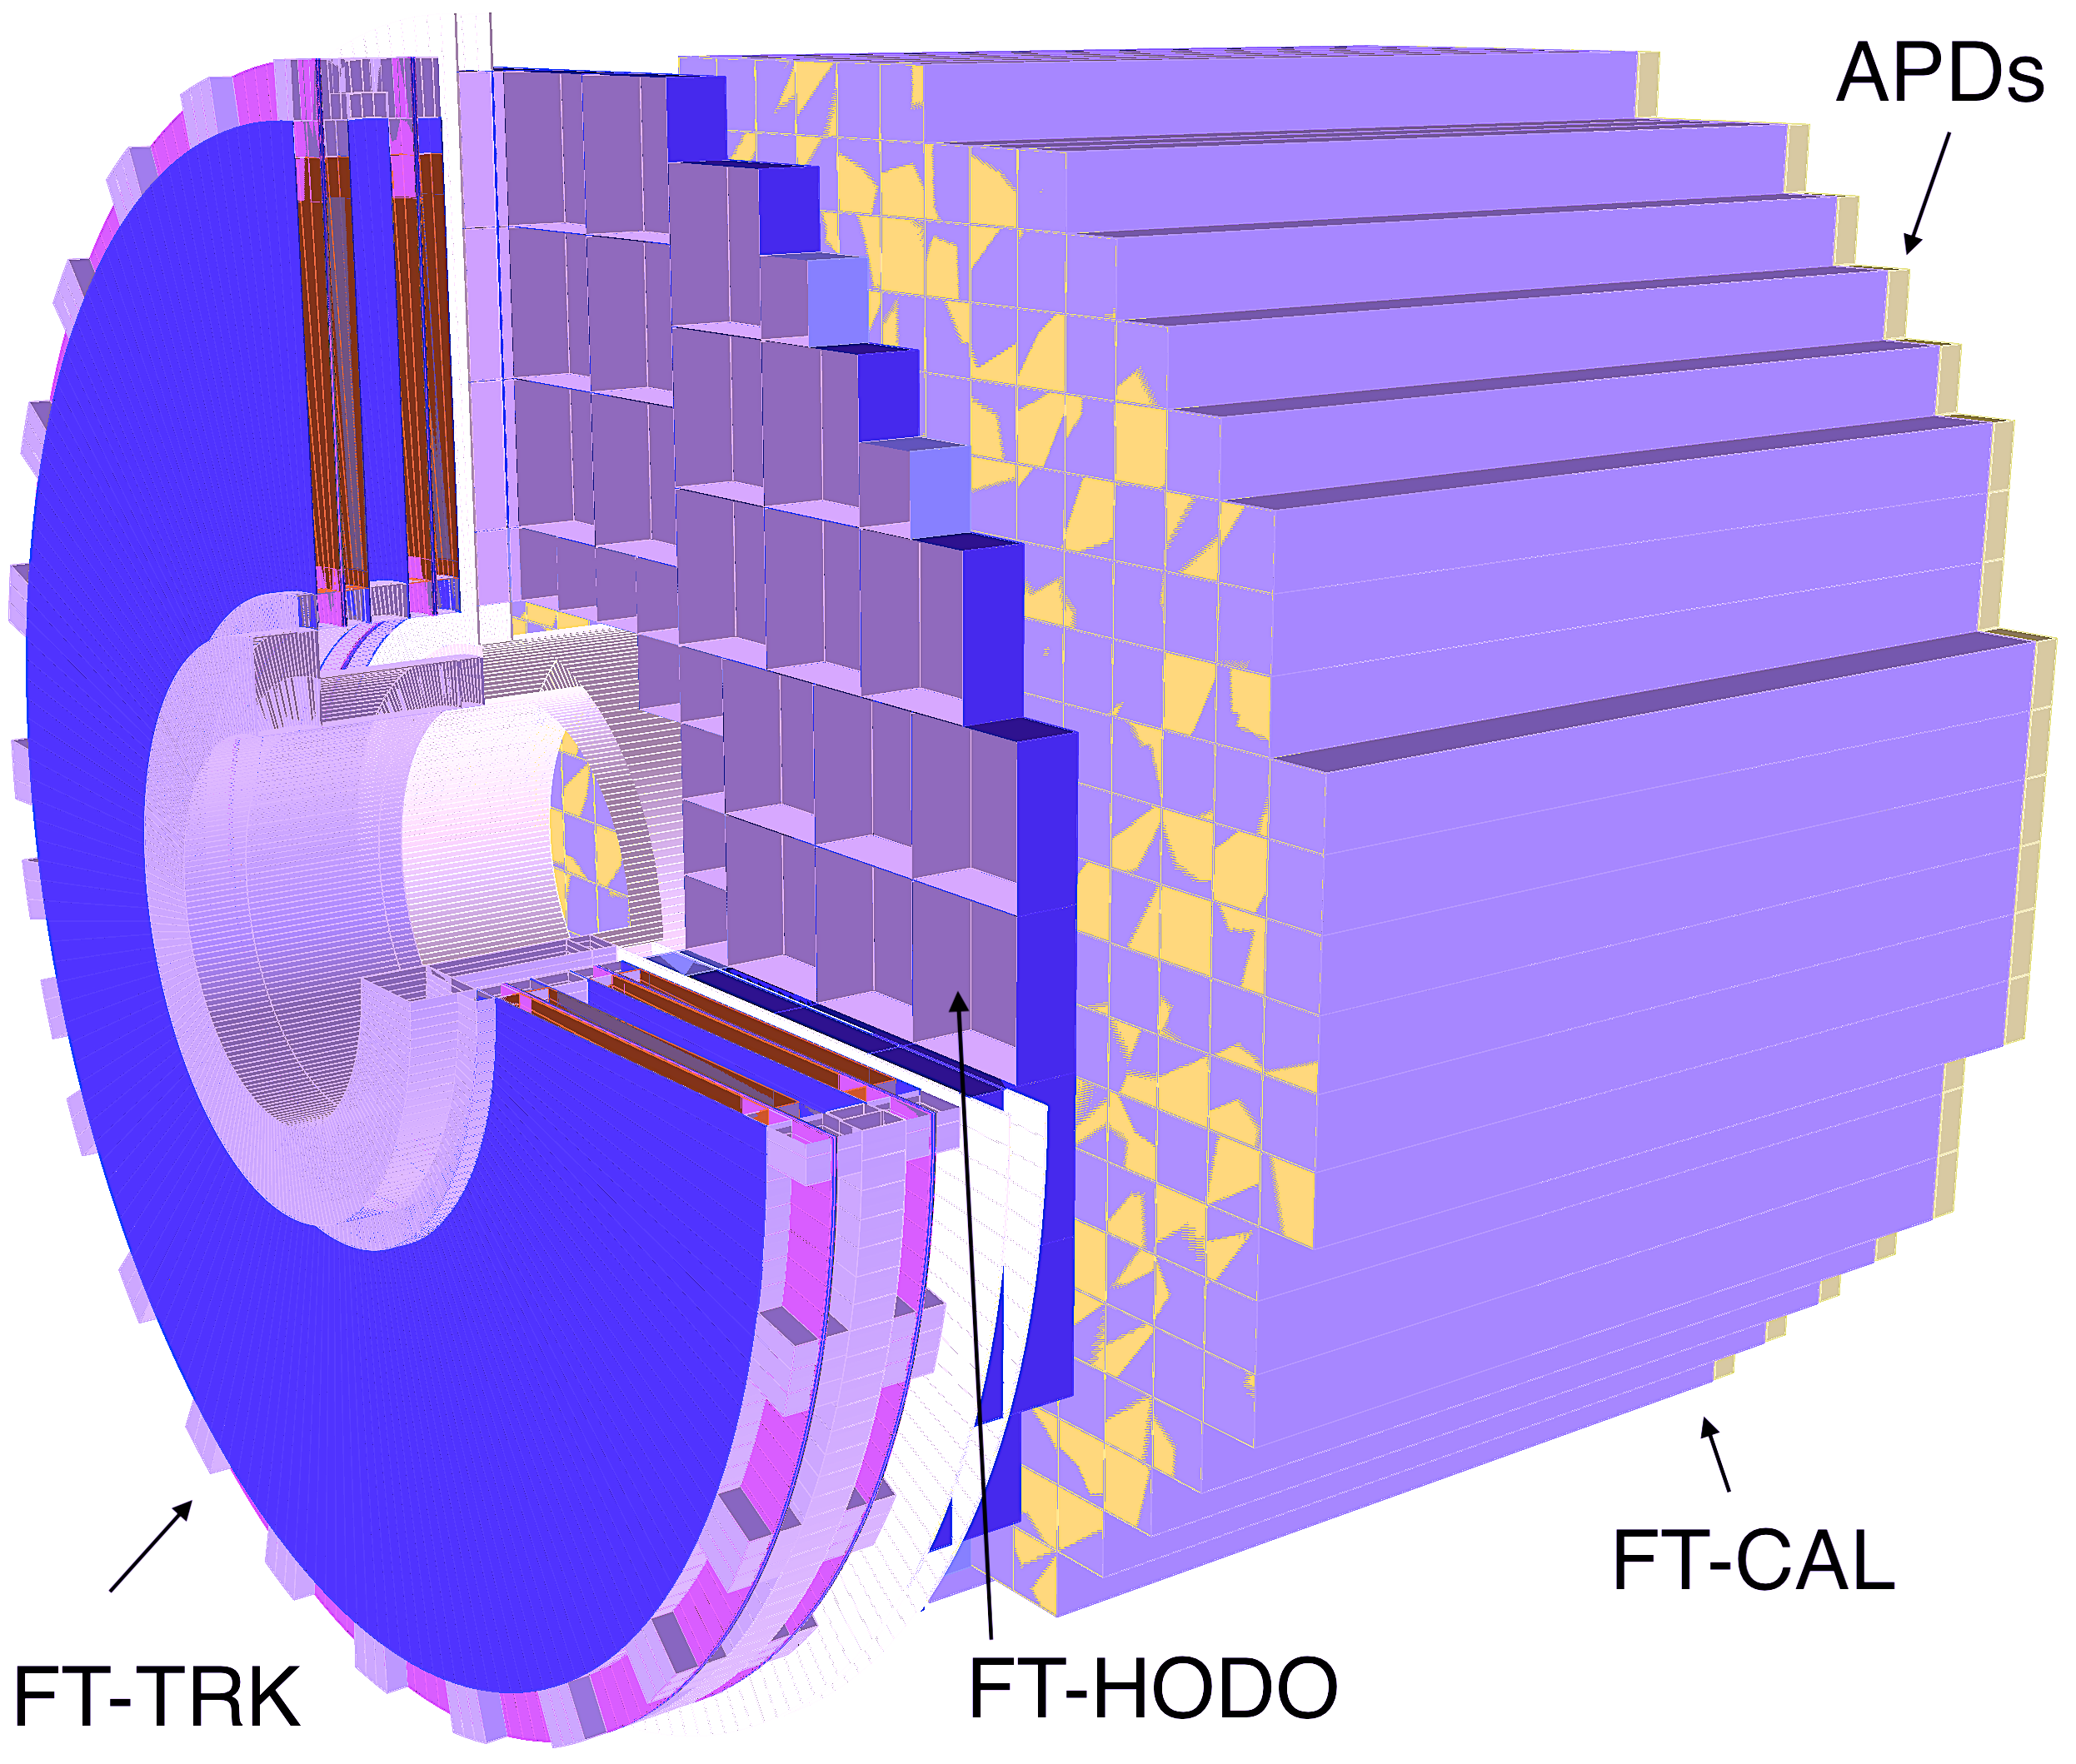
\includegraphics[width=0.99\columnwidth,keepaspectratio]{img/ftDetails.png}
	\caption{Top: the FT detector implementation in GEMC. The boxes surrounding FT-CAL contain the electronics.
			 Bottom: details of the the three subsystems implementation. As seen by the beam (impinging from the left):
             the disks form the FT-TRK; the FT-HODO scintillators just behind the tracker;
			 and the FT-CAL crystals. }
	\label{fig:ftGeometry}
\end{figure}

The FT-TRK digitization provides the ADC value calculated using the total energy deposited (after hit sharing).
There is no timing information in the FT-TRK output.

For FT-CAL hits, the energy deposited is converted first to the charge produced at the end of the electronics chain composed
by an avalanche photodiode (APD) and pre-amplifier, and then to an ADC.
The first conversion is based on the measured charge for cosmic rays that deposit a known energy in the crystals,
while the second conversion is based on the FADC conversion factor. A smearing on the final ADC values is added,
accounting for the Poisson distribution of photo-electrons produced by the photosensor, the Gaussian noise of the
photosensor, and of the preamplifier. All parameters, the number of photo-electrons per MeV of energy deposited,
the RMS width of the APD noise, and of the preamplifier input noise, have been tuned to the experimental data.

The same approach is adopted to process FT-HODO hits, in which the deposited energy is first converted to charge and then to ADC.
The smearing in this case accounts only for the Poisson distribution of the measured number of photo-electrons,
which dominates over other sources because of the relatively small number of photo-electrons per MeV of energy deposition.

The TDC of FT-CAL hits is computed from the time of the energy deposition, accounting for the speed of the scintillation light in
the crystal and the distance to the photosensor, assuming a known time-to-TDC conversion factor. A Gaussian smearing on the
resulting TDC is added based on a fixed RMS resolution derived from the experimental measurements.

Similarly, the TDC of FT-HODO hits is derived from the time of a given energy deposition, adding a fixed offset before the
conversion from time to TDC and a Gaussian smearing. As in previous cases, all relevant parameters have been tuned to the
observed detector response.
The digitized output bank variables are summarized in Table \ref{tab:ftBank}

\begin{table}[h]
	\begin{center}
		\begin{tabular}{| c | c | c |}
			\hline \hline
			Variable            & Description      \\
			\hline
		                         & Tracker         \\
			\hline
                         sector  &     sector      \\
                          layer  &      layer      \\
                      component  &  component      \\
                            ADC  &        ADC      \\
			\hline
		                         & Hodoscope       \\
			\hline
						 sector  &     sector      \\
                          layer  &      layer      \\
                      component  &  component      \\
                            ADC  &        ADC      \\
                            TDC  &        TDC      \\
			\hline
								 & Calorimeter     \\
			\hline
				         sector  &     sector      \\
				   	      layer  &      layer      \\
					  component  &  component      \\
							ADC  &        ADC      \\
							TDC  &        TDC      \\
			\hline \hline
		\end{tabular}
	\end{center}
	\caption{The digitized FT banks for the tracker, hodoscope, and calorimeter}\label{tab:ftBank}
\end{table}

\noindent The time window  of the Tracker is set to to 132 ns: all Geant4 steps within the same strip and time window are collected in one hit.
The time window of the hodoscope and calorimeters are set to 400 ns: all Geant4 steps within the same paddles and time window
will be collected on one hit in each system.

\subsection{Event Builder}
\label{sec:eb}

The Event Builder is the last service in the reconstruction algorithm, and performs a series of functions:

\begin{itemize}
    \item collects information from the upstream services;
    \item correlates information from the sub-detectors into particles;
    \item performs a general particle identification scheme;
    \item organizes the resulting information into a standardized, persistent data bank structure.
\end{itemize}

The service is run twice with identical algorithms, once using hit-based tracks, and later with time-based tracks,
where the results of the hit-based Event Builder are used to initialize time-based tracking.

\subsubsection{Forming Particles}

In defining a reconstructed charged particle in CLAS12, the Event Builder assumes that an assignment will be
made for each reconstructed track in both the Forward Detector and the Central Detector. The associated
calorimeter, scintillator, and Cherenkov detector responses are then assigned to that particle based on
geometric coincidences between the detector responses and the track, with matching criteria corresponding
to the resolution of a given detector. The geometric matching is based on the distance of closest approach
between the track and the response, where an example is shown in Fig.~\ref{fig:ebmatch}.

A similar procedure is followed for creating neutral particles, except the seeding is presently with
unassociated ECAL (for the Forward Detector) and CND (for the Central Detector) responses instead of tracks.

\begin{figure}
\centering
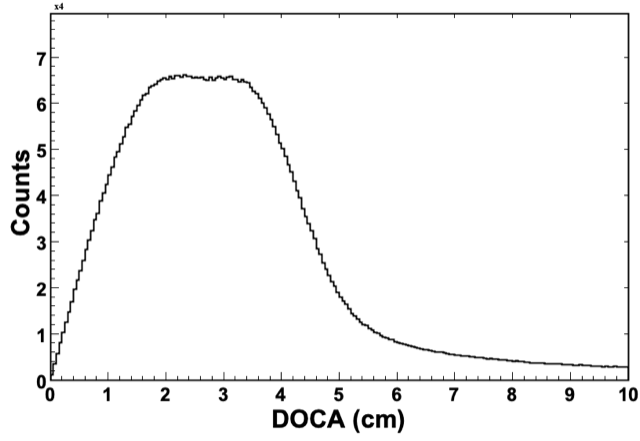
\includegraphics[width=0.45\textwidth,height=0.2\textheight]{pics/pcal-doca.png}
\caption{Example of the geometric matching criteria showing the distance of closest approach between a charged
  track from the DC extrapolated to the ECAL and the cluster positions in the ECAL.}
  \label{fig:ebmatch}
\end{figure}

\subsubsection{Event Start Time}

A start time is assigned to the entire event and serves as our most precise reference time on which all time-based
particle identification relies. This is based on the optimal charged particle candidate in the Forward Detector with
an associated FTOF timing response. The Event Builder assigns the start time based on the highest energy electron
in the ECAL. If there is no electron in the ECAL, it next looks for a positron in the ECAL. If there is no lepton, the
next track in the priority list is a forward-going positive track (assumed to be a $\pi^+$). Finally, if there is no
forward-going positive track, it looks for a forward-going negative track (assumed to be a $\pi^-$). When looking
for $\pi^+$ or $\pi^-$ tracks, only the candidate with the highest momentum in each group is considered.

A parallel event start time is determined from the FT to facilitate physics analyses and triggers where the
primary scattered electron is at very forward angles in the FT. In this case, all combinations of charged particles
in the FT and the Forward Detector are considered. The particle in the FT is assumed to be an electron, whereas
all hadron mass hypotheses are considered for the Forward Detector tracks. The combination with the best time
coincidence is chosen. The timing of the resulting FT electron is then used to assign the start time.

A correction to the start time is then performed using the RF signal from the accelerator, combined with the
reconstructed event vertex position. This effectively aligns the event start time to our best measure of the
beam-bunch arrival time at the target.

The uncorrected, measured vertex time of a particle, $t_v$, can be written as
\begin{equation}
    t_v = t-\frac{P_L}{\beta c},
\end{equation}

\noindent
where $t$ is the measured time response (e.g. in a scintillator), $P_L$ is the path length between the primary
interaction vertex and that response, and $\beta c$ is the speed of the particle.  We can then construct a
correction to align this time with the closest beam bunch time at the target:

\begin{eqnarray}
\Delta t_{RF}\!\!\!\!&=&\!\!\!\! t_v + (z_0-z_v)/c - t_{RF} - N/(2 f_{RF}),\\
\Delta t'_{RF}\!\!\!\!&=&\!\!\!\! mod(\Delta t_{RF},1/f^{RF})-1/(2 f_{RF}),  \nonumber
\end{eqnarray}

\noindent
where $f_{RF}$ is the frequency of the accelerator, {\color{red}249.5~MHz or 499~MHz, corresponding to 2.004~ns or 4.008~ns bunch
spacings}, $t_{RF}$ is the measured, calibrated RF time for the event, and $z_0$ is the target center and enters
due to its use as a position calibration reference. The resulting RF- and vertex-corrected start time for the event
is then given as

\begin{equation}
  \label{eq:starttime}
t'_v = t_v - \Delta t'_{RF}.
\end{equation}

\subsubsection{Particle Identification}

The next stage is a basic particle identification scheme.  This is intended to be loose to accommodate a variety of
physics analyses, while persisting the necessary information to easily tighten and improve the criteria later.

For charged particles, first calorimetry and Cherenkov information is used to positively identify $e^-/e^+$
candidates in the Forward Detector. If the measured energy deposition is consistent with the expected sampling
fraction of the ECAL, and the photoelectron response from the HTCC is consistent with $\beta\sim1$, the particle
is assigned as an $e^-$ or $e^+$ depending on sign of the curvature of the track from forward tracking with the
DCs through the torus magnetic field. {\color{red}\sout{In a subsequent particle identification stage, additional information from the
ECAL shower profile must be considered for momenta above $\sim$4.5~GeV where the HTCC becomes sensitive to
charged pions. The basic particle identification scheme in this regime is insufficient to separate $e^-/\pi^-$ and
$e^+/\pi^+$.}}

The remaining charged particles are then assumed to be hadrons and assigned an identity based solely on timing
information, where the $p/K/\pi$ candidate giving the smallest time residual is assigned. This time residual is
computed from the difference between the measured particle flight time and that computed for a given mass
hypothesis. Figure~\ref{fig:betavsp} shows reconstructed $\beta$ vs. momentum distributions from beam data
for forward-going positively charged hadrons using information from the FTOF and DC subsystems, where the
electron is reconstructed either in the Forward Detector (Fig.~\ref{fig:betavsp}(top)) or in the Forward Tagger
(Fig.~\ref{fig:betavsp}(bottom)). The computed curves for the different mass hypotheses are overlaid.

{\color{red}\sout{ Due to the inherent time resolutions of the FTOF and CTOF systems, the charged particle bands seen in the
$\beta$ vs. $p$ plots (e.g. see Fig.~\ref{fig:betavsp}) begin to overlap for $\pi/K$, $\pi/p$, and $K/p$ as
the track momentum increases. Therefore, the basic particle identification scheme is not sufficient to rely on
for physics analyses. The identification scheme must be supplemented by information from other detector
subsystems where available, for example using the LTCC and RICH detectors in the forward direction. Further
improvements in the particle identification assignments can be made using constraints from exclusive event
reconstruction using the missing mass technique and/or event kinematic fitting. Of course it is essential for
physics analyses that the Monte Carlo simulation of CLAS12 is matched closely to the actual detector energy and
timing responses in order to match the particle identification responses for misidentification and purity.}}

\begin{figure}[t]
\centering
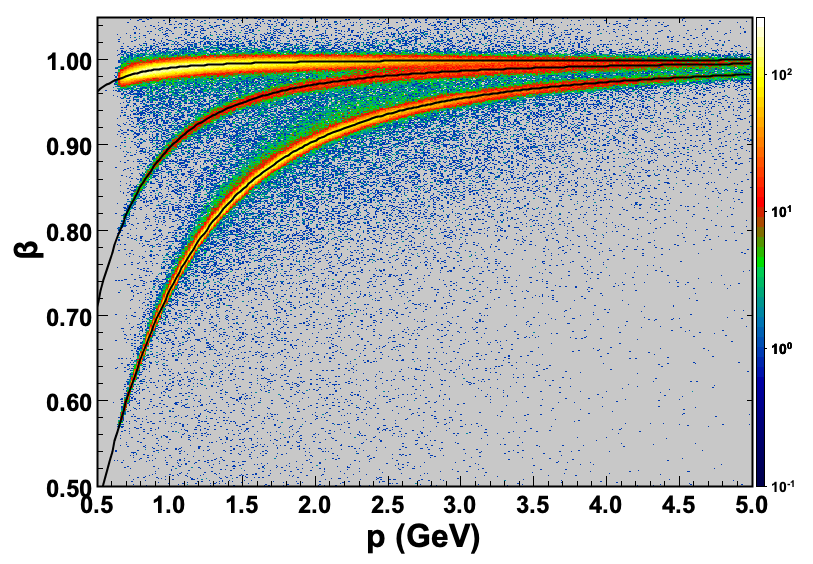
\includegraphics[width=0.45\textwidth]{pics/ftof_betap.png}
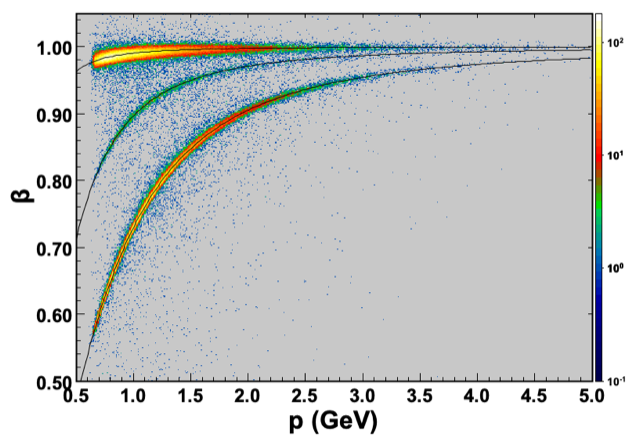
\includegraphics[width=0.45\textwidth]{pics/ft_betap.png}
\caption{Particle $\beta$ vs. momentum from simulation data for positively charged tracks with their start time
  from an electron in the Forward Detector (top plot) or in the FT (bottom plot).}
\label{fig:betavsp}
\end{figure}

For neutral particles, particle identification is assigned only for neutrons and photons, based only on timing and
topological information. {\color{red} For the Forward Detectors this is presently based on the ECAL, while for the Central
Detector it is presently based on the CND. The reconstructed cluster position is used to compute the particle
travel path from the vertex of the event, defined as the vertex of the trigger particle (an electron or charged hadron n the Forward Detector).
If the particle timing and travel path results in $\beta\sim$1, it is assigned as a photon, otherwise it
is assigned as a neutron. The $\beta$ threshold for the PID assignment is a parameter read from the database.} For photons in the Forward Detector, the momentum is then assigned
using the reconstructed ECAL energy and accounting for the calorimeter sampling fraction~\cite{ecal-nim}. For
neutrons, the momentum is assigned based on the measured $\beta$ and the neutron mass.
Figure~\ref{fig:neutbeta} shows an example of $\beta$ reconstructed for neutrals in the Forward Detector
showing separation of photons and neutrons.

\begin{figure}
\centering
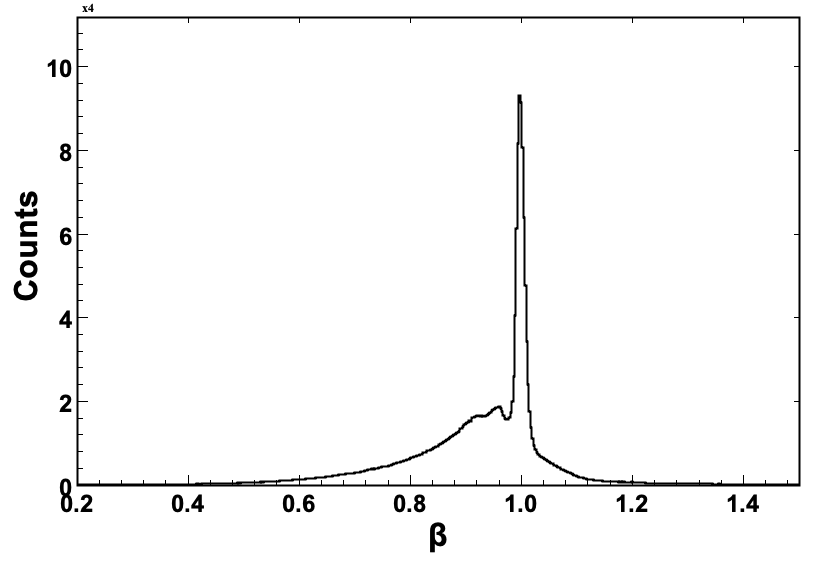
\includegraphics[width=0.45\textwidth]{pics/neutral_beta.png}
\caption{$\beta$ distribution for neutral particles as measured by the ECAL from simulation data, showing a sharp
  peak at $\beta=1$ from photons and a broader, slower distribution from neutrons.}
\label{fig:neutbeta}
\end{figure}

A particle identification quality factor in the form of a signed-$\chi^2$ is assigned based on the individual
contributing detector subsystem responses and their resolutions. For $e^-/e^+$ identification the
resolution-normalized distance from the expected ECAL sampling fraction is used, while for charged hadrons the
resolution normalized time-difference is used. The resulting information is organized into standardized output
bank structures for physics analysis, see Section~\ref{sec:dsts}. This includes the particle four-vectors, the
associated detector responses, and global event information such as beam RF and helicity information.

\subsubsection{Particle Identification Performance}

The accuracy of the particle identification algorithm that is currently implemented can be estimated from
Monte Carlo simulations where the assigned particle identification can be compared to the true one.
Tables~\ref{table:pidmatrix} and~\ref{table:pidmatrix2} show the particle identification matrix for the Forward
and Central Detectors, respectively. The values are based on simulations of electron-hadron or electron-photon
pairs with hadron and photon momenta in the range from 1 to 2.5~GeV and electron momenta in the range from 1 to
9~GeV. The diagonal elements correspond to the cases where the particle is correctly identified and the off-diagonal
elements to the cases where the particle is misidentified. It should be noted that the resulting values are strictly
related to the assignment algorithm currently in use and on the timing resolutions implemented in the Monte Carlo
simulation~\cite{sim-nim}. An increase of the diagonal element values and a corresponding decrease of the
misidentification probability is expected as, for example, information from the threshold Cherenkov detectors and
the RICH in particular are integrated into the algorithm and isolated hits in the FTOF and CTOF detectors are
incorporated into the neutral particle identification algorithm.

\begin{table}[ht]
  \begin{center}
    \begin{tabular}{|c|cccccc|}\hline
          & \multicolumn{6}{c|}{Truth}\\        
          & $e$  & $\pi$ & $K$  & $p$  & $n$  & $\gamma$ \\\hline
  $e$     & 0.98 &       &      &      &      &          \\ 
  $\pi$   &      &  0.93 & 0.10 & 0.00 &      &          \\ 
  $K$     &      &  0.03 & 0.80 & 0.00 &      &          \\ 
  $p$     &      &  0.03 & 0.02 & 0.98 &      &          \\ 
  $n$     &      &       &      &      & 0.66 &   0.01   \\ 
 $\gamma$ &      &       &      &      & 0.14 &   0.95   \\\hline 
    \end{tabular}  
    \caption{Particle identification matrix for the CLAS12 Forward Detector based on simulated hadrons and
      photons with momentum between 1 and 2.5~GeV, and electrons up to 9~GeV. The diagonal elements are
      correctly identified, while the off-diagonal elements are misidentified. Detector inefficiencies are included.}
  \label{table:pidmatrix}
  \end{center}
\end{table}

Another measure of the particle identification performance for neutrals is given by the reconstruction of $\pi^0$
decays to two photons. Figure~\ref{fig:pi0mass} shows the $\gamma \gamma$ invariant mass reconstructed from
the ECAL and from the Forward Tagger.

\begin{table}[ht]
  \begin{center}
    \begin{tabular}{|c|cccc|}\hline
          & \multicolumn{4}{c|}{Truth}\\        
          & $\pi$ & $K$  & $p$  & $n$  \\\hline
  $\pi$   &  0.84 & 0.14 & 0.00 &      \\ 
  $K$     &  0.11 & 0.80 & 0.01 &      \\ 
  $p$     &  0.03 & 0.04 & 0.95 &      \\ 
  $n$     &       &      &      & 0.11 \\ 
 $\gamma$ &       &      &      & 0.00 \\\hline 
    \end{tabular}  
    \caption{Particle identification matrix for the CLAS12 Central Detector based on simulated hadrons with momentum
      between 0.3 and 1.1~GeV. The diagonal elements are correctly identified, while the off-diagonal elements
      are misidentified. Detector inefficiencies are included.}
  \label{table:pidmatrix2}
  \end{center}
\end{table}

\begin{figure}[t]
\centering
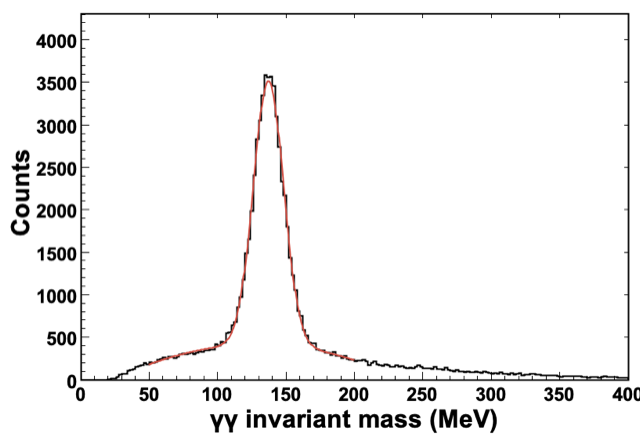
\includegraphics[width=0.45\textwidth]{pics/ecal_pi0.png}
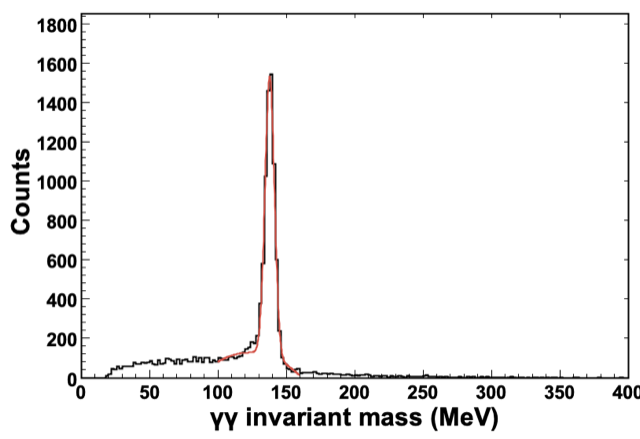
\includegraphics[width=0.45\textwidth]{pics/ft_pi0.png}
\caption{Reconstructed $\pi^0 \to \gamma \gamma$ candidates using photons detected in the ECAL (top plot) and
  the FT (bottom plot). The plots are based on simulations of semi-inclusive deep inelastic scattering events
  generated based on the PYTHIA event generator~\cite{clasdis}.}
\label{fig:pi0mass}
\end{figure}


\section{Data Processing}
\label{sec:dataproc}

\subsection{Workflow}

The raw data is currently first preprocessed.  This is an I/O-heavy, single-threaded process and involves
extracting hits from waveforms, translating data-acquisition/hardware nomenclature to physical detector objects,
performing special analyses dependent on serial event access, and converting from the input EVIO format to the
HIPO data format.  This phase includes registering beam helicity state changes and special scaler events, and
populating their results into tag-1 HIPO events to facilitate later analysis.  The result is a factor of $\sim$5
reduction in size and a file format optimized for I/O.

The second stage is a CPU-heavy reconstruction phase, including all of the tracking, clustering, calorimetry,
time-of-flight, and event building in the previous sections.  It runs multi-threaded in the CLARA framework and
can be configured to output various data schema depending on the purpose, see Section~\ref{sec:dsts}, during
full-scale data processing, or larger, special-purpose banks during preliminary calibration phases.

The final stage of data processing involves the running of I/O-heavy analysis trains that perform event skimming
(e.g. filtering out specific final state event topologies),  and accommodate various corrections and common analysis
plugins.  It splits the data into multiple output files based on different event selections, each optimized for a
group of physics analyses. An example schematic is shown in Fig.~\ref{fig:train}. This stage is designed to be run
repeatedly as selection criteria and physics analyses mature.

\begin{figure}
    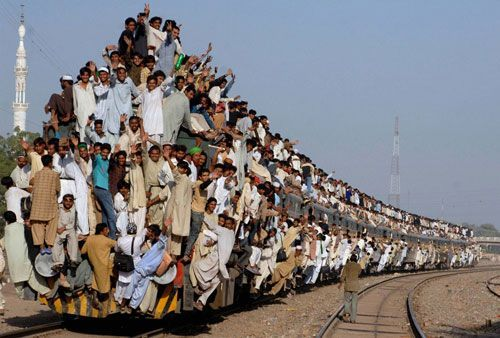
\includegraphics[width=0.45\textwidth,height=0.2\textheight]{pics/train.jpg}
    \caption{Schematic flow of analysis trains.\label{fig:train}}
\end{figure}

\subsection{Data Summary Tapes}
\label{sec:dsts}

The final data output is provided by the Event Builder in the form of data summary tapes (DSTs), a standardized
selection of HIPO banks for physics analysis. These include:

\begin{itemize}
\item global event information, e.g. run number and event timestamp, integrated beam charge, beam helicity state,
  event start time;
\item particle information, e.g. momentum four-vector and vertex position, particle type and identification quality,
  and status words that encode information on the sub-detectors involved in the particle formation;
\item high-level detector response information associated with each particle, e.g. detector identifier, response
  position and time, and track trajectory in each detector layer.
\end{itemize}

\noindent
The DST banks are organized such that the large, detector information can easily be dropped to leave only the data
essential for a high-level physics analysis, without leaving dangling references or unnecessary information.

\subsection{Computing Resources}

Reconstruction of all CLAS12 data is performed on Jefferson Lab's batch computing system~\cite{jlab-batch-farm}.
It currently consists of about 400 compute nodes of various flavors, with a total of about 21,000 available jobs
slots and half as many cores.  The input raw data and analyzed output data are stored on JLab's tape silo
\cite{jlab-tape-silo}, which provides sufficient cold storage for all of JLab's activities.  Data for physics analysis is
also stored live on JLab's Lustre filesystems~\cite{jlab-lustre}, which is currently about 2~PB of disk, but will be
increased to almost 7~PB in the near future. Analysis of reconstructed data is performed on the JLab batch and
interactive farm nodes, and also exported to other institutions for final physics analysis.

\section{Code Management}

\subsection{Repositories}
The software is managed in a github repository \cite{recon-github}, and branches and forks are utilized to accommodate parallel development by many groups.  Two main branches, {\it master} and {\it development}, are utilized to store code ready for production and for validation, respectively. For the main branches, all modifications are made only through pull requests after passsing the automated tests in Section \ref{sec:tests} and require a approval by a software expert.

\subsection{Releases}
There are four release types; major release, interface change release, bug-fix
and test releases.  A numbering scheme is implemented to indicate the type of change.
Releases that are ungoing a validation period carry a letter that indicates the type of validation:
for production or a special algorithm study.

Major release:
- Previous productions likely are obsolete.
- Introducing new technology, major algorithmic improvements, or
schema changes that make previous productions obsolete.
- Impact for users: maximal
- Impact for developers: maximal

Interface change release
- The release contains changes that make the program not backwards compatible.
- Releases for clean-up operation with changes in users' interfaces of
packages, for design iteration that affect the users' interface, and
for re-packaging and simple schema changes.
- Not backwards compatible
- Impact for users: large (Need adapt their code to new interfaces.)
- Impact for developers: large (Need adapt their code to new interfaces.)

Bug-fix and new feature release
- Extensions of interfaces and new implementations are allowed, while
backwards compatibility of interfaces is guaranteed.
- Impact for users: small (Need to compile against a new area.)
- Impact for developers: small

Fast bug-fixes and test releases
- Impact for users: none
- Impact for developers: If their development depends on the fix, they will checkout
and compile the fixes in their local area.
- bug-fixes are at the at sub-system level.
- they are reflected in sub-system level letter tags only.

Fast fixes are collected in regular intervals into bug-fix releases.

\subsection{Code tests and validation}\label{sec:tests}
In addition to automatic builds, the software includes both basic unit tests and advanced tests for several packages. Unit tests are designed to verify the correctness and reproducibility of the reconstruction output for a specific package. This involves for example reconstructing a simulated track or particle hit in a specific detector and comparing the result to the true information. Advanced and extended tests are, on the contrary, designed to verify the correctness and reproducibility of the overall event reconstruction on both simulated and real data sample by comparing to the true information in the first case or to the results obtained in previous releases in the second case. A portion of the tests are run automatically at the build time, using the TravisCI system linked to the github repositories.  These automatic tests take about 30 minutes to run and have proven invaluable in overseeing and improving software development.

In addition to unit and advanced tests, every new release is subject to extensive validation on both simulated and real data. For this purpose, samples of Monte Carlo and real events for different beam energies and detector configuration were chosen to provide an extensive test of event reconstruction over the whole detector acceptance. Reconstruction of these samples is performed and results are compared to previous code releases. The comparison focuses on several parameters, from processing time, to resolution and efficiencies for particle reconstruction. A new release is accepted for production only if it is meeting predefined criteria on these observables and is globally giving improved performances. 
% CLAS12 Software must be accurate. Under the software, we assume physics data processing (PDP) applications like reconstruction, simulation and calibration. PDP applications, developed using the CLAS12 software framework, consist of services that run in a context that is agnostic to the global application logic. So, the CLAS12 software accuracy depends on accuracy of services used in designing the PDP application. In order to be part of the production service inventory, each service must have self accuracy and efficiency testing routines.
\section{Ongoing Developments}

The software framework and event reconstruction described in the previous sections are based on the code that
is currently being utilized for data processing or will be deployed in the near future in an upcoming release.
Nevertheless, as CLAS12 data are being analyzed, several potential improvements have been identified and are
either in the process of being implemented or planned for the near future. In this section, we discussed the most
relevant developments.

\subsection{Artificial Intelligence Assisted Forward Tracking}

Recent progress in the field of machine learning offers a promising alternative to conventional algorithmic tracking
methods. While the conventional methods provide algorithms that are well understood and well studied, there are
some algorithms in the data reconstruction process that can be substituted with neural networks to reduce data
processing times. For CLAS12, tracking is the most time-consuming aspect of experimental data processing.
Tracking in the DC takes up to $\sim$90\% of the total data processing time, which includes finding track
candidates and iterating through track-forming segments to find the best combinations of segments that can form
a track. This time increases with luminosity as the number of noise segments increases and can ultimately lead to
processing time degradation. We have started to address this issue by employing machine learning techniques
to find the best track candidates in each event and to reduce the number of combinatorics.

With increased luminosity, the number of potential DC cross candidates increases. This implies that the Kalman
Filter fitting algorithm must be run for all possible combinations of crosses. 

Reconstructed track segments from both positive and negative tracks from the currently reconstructed data
samples are used to train the neural network. We are currently testing three types of neural networks: boosted
decision tree~\cite{bdt}, multilayer perceptron~\cite{mp}, convolutional~\cite{cnn}. 

Preliminary results indicate that the convolutional neural network performed competitively with the multilayer
perceptron with about 97\% accuracy and 3\% false positives. 

The hits identified as on-track by the neural network are saved in a bank and the DC reconstruction package was
adapted to read these data as an input to hit-based tracking. Benchmark results of reconstruction speed for
hit-based tracking show a factor of $\sim$5 improvement.

Implementing the neural network software into the CLAS12 reconstruction workflow is under development.
The second stage of the machine learning project will concentrate on efficiency improvements using artificial
intelligence assisted tracking.

\subsection{Improvements to Event Reconstruction}

The CLAS12 detector began beam operations for physics in early 2018 after a several month commissioning
phase. Since that time the event reconstruction code has continued to improve to meet issues as they have
arisen. However, the code and the framework are already performing well enough for advanced physics
analysis of the collected data to proceed. A broad survey of reconstruction results using the current CLAS12
software framework and event reconstruction code are presented based on beam data in Ref.~\cite{clas12-nim}.
As might be expected, there are still areas where development, testing, and validations are in progress in
order to continue improvements. In this section, several areas of ongoing work are highlighted.

\subsubsection{Improvements to Central Tracking}

Improvements to tracking in the CVT are currently being studied. These include:

\begin{itemize}
\item improvements to the tracker geometry implementation and fitting algorithm - the combination of these
  code modifications is expected to improve the fit residuals, which are indicative of a bias in the current
  version of the code as seen through systematic shifts in their distributions;
\item implementation of geometrical distortions derived from detector alignment;
\item the use of the beam offset information (relative to the nominal beam $z$-axis) in the track fit initialization;
\item the use of SVT clusters instead of crosses in the seeding.
\end{itemize}

These updates aim at enhancing the robustness of the tracking algorithm and improving resolution and efficiency.

\subsubsection{Improvements to Time-of-Flight Reconstruction}

As discussed in Section~\ref{tof-sys}, the output of the time-of-flight reconstruction are hits that are used
as input to the Event Builder algorithms. The use of clusters for particles that go through two adjacent TOF
paddles (either in the FTOF or CTOF systems) is expected to yield improved timing resolution, as is combining
the hit times in FTOF for tracks that go through both forward counter hodoscopes as discussed in
Section~\ref{sec:tof-cluster}. A quantitative estimate of the timing resolution improvements and a validation of
the clustering algorithm are currently ongoing using on Monte Carlo simulations.

\subsection{Improvements to the Event Builder}\label{sec:eb:improvements}

The matching of tracks to detector responses is currently based on the distance of closest
approach between the tracks and the response coordinates. Improvements to this matching may be obtained using
track trajectories, i.e. intersections of the track with the relevant detector planes where the responses are reported,
potentially reducing the uncertainty on the path length determination that relies on the response
coordinates.  Additionally, the use of timing information in matching will reduce the effect of accidentals in high rate detectors
such as the HTCC.

In the future, the particle identification scheme will be improved by exploiting additional detector information. This
includes the ECAL shower profile to improve electron-pion separation for momenta above $\sim$4.5~GeV where the
HTCC becomes sensitive to charged pions, and RICH responses to improve charged-particle identification in the
forward direction.


\section{Conclusions}

We have presented the software framework and event reconstruction that are currently being utilized for the processing of data collected by the CLAS12 experiment, in Hall B at Jefferson Lab.  

The framework was developed to allow processing of CLAS12 data for reconstruction and analysis purposes with an elastic, eclectic, and expandable approach thanks to the service-oriented architecture. The specific software applications leverage on an extensive set of common libraries for handling I/O, geometry, databases and magnetic field, designed to support data monitoring, calibration, reconstruction and analysis.

Full event reconstruction is implemented in the framework as a chain of micro-services that perform reconstruction of the individual CLAS12 sub-systems and whose output information is collected by the Event Builder service to form and identify particles. While the current reconstruction chain already supports reconstruction of all the sub-system and creation of full events, upgrades to the existing software implementation and algorithms are being studied.

\section{Acknowledgments}

This work was supported in part by the Chilean Comisi\'on Nacional de Investigaci\'on Cient\'ifica y Tecnol\'ogica
(CONICYT), the Italian Istituto Nazionale di Fisica Nucleare, the French Centre National de la Recherche Scientifique,
the French Commissariat \`{a} l'Energie Atomique, the U.S. Department of Energy, Office of Science, Office of
Nuclear Physics under contract DE-AC05-06OR23177, the National Science Foundation, the Scottish Universities
Physics Alliance (SUPA), the United Kingdom's Science and Technology Facilities Council, and the National Research
Foundation of Korea.

\begin{thebibliography}{99}

\bibitem{clas12-nim}
V.D. Burkert {\it et al.}, ``The CLAS12 Spectrometer at Jefferson Laboratory'', to be published in Nucl.
Inst. and Meth. A, (2020). (see this issue)

\bibitem{dc-nim}
M.D. Mestayer {\it et al.}. ``The CLAS12 Drift Chamber System'', to be published in Nucl. Inst. and
Meth. A, (2020). (see this issue)

\bibitem{ltcc-nim}
M. Ungaro {\it et al.}, ``The CLAS12 Low Threshold Cherenkov Counter'', to be published in Nucl. Inst.
and Meth. A, (2020). (see this issue)

\bibitem{htcc-nim}
Y. Sharabian {\it et al.}, ``The CLAS12 High Threshold Cherenkov Counter'', to be published in Nucl. Inst.
and Meth. A, (2020). (see this issue)
  
\bibitem{rich-nim}
M. Contalbrigo {\it et al.}, ``The CLAS12 RICH Detector'', to be published in Nucl. Inst. and
Meth. A, (2020). (see this issue)

\bibitem{ftof-nim}
D.S. Carman {\it et al.},   ``The CLAS12 Forward Time-of-Flight System'', to be published in Nucl.
Inst. and Meth. A, (2020). (see this issue)

\bibitem{ecal-nim}
G. Asryan {\it et al.}, ``The CLAS12 Forward Electromagnetic Calorimeter'', to be published in Nucl. Inst. and
Meth. A, (2020). (see this issue)

\bibitem{svt-nim}
A. Antonioli {\it et al.}, ``The CLAS12 Silicon Vertex Tracker'', to be published in Nucl. Inst. and
Meth. A, (2020). (see this issue)

\bibitem{mm-nim}
A. Acker {\it et al.}, ``The CLAS12 Micromegas Vertex Tracker'', to be published in Nucl. Inst. and
Meth. A, (2020). (see this issue)

\bibitem{ctof-nim}
D.S. Carman {\it et al.}, ``The CLAS12 Central Time-of-Flight System'', to be published in Nucl.
Inst. and Meth. A, (2020). (see this issue)

\bibitem{cnd-nim}
P. Chatagnon {\it et al.}, ``The CLAS12 Central Neutron Detector'', to be published in Nucl. Inst. and
Meth. A, (2020). (see this issue)

\bibitem{ft-nim}
A. Acker {\it et al.}, ``The CLAS12 Forward Tagger'', to be published in Nucl. Inst. and
Meth. A, (2020). (see this issue)

\bibitem{clara-2011}
V. Gyurjyan {\it et al.}, CLARA: A Contemporary Approach to Physics Data Processing, J. Phys. Conf. Ser.
{\bf 331}, 032013 (2011).

\bibitem{clara-service}
J. Carbonneau, M. Moog,  J. Gilfoyle, {\it et al.}, 2011 APS Division of Nuclear Physics Meeting Abstracts, EA.024.

\bibitem{framework}
Component Based Dataflow Processing Framework, 2015, IEEE DOI: 10.1109/BigData.2015.7363971,
ISBN: 978 1-4799-9926-2

\bibitem{clara-2016}
CLARA: The CLAS12 Reconstruction and Analysis framework, 2016, J. Phys. Conf. Ser. {\bf 762}, 012009 (2016).

\bibitem{gluex}
The GlueX Collaboration, The GlueX Experiment in Hall~D, Presentation to JLAB PAC36, (2010.
http://www.gluex.org/docs/pac36\_update.pdf

\bibitem{magnets-nim}
R. Fair {\it et al.}, ``The CLAS12 Superconducting Magnets'', to be published in Nucl. Inst.
and Meth. A, (2020). (see this issue)

\bibitem{evio}
Event IO Data Format, \\ https://coda.jlab.org/drupal/content/event-io-evio

\bibitem{daq-nim}
S. Boyarinov {\it et al.}, ``The CLAS12 Data Acquisition System'', to be published in Nucl. Inst. and
Meth. A, (2020). (see this issue)

\bibitem{spiri}
Alexander Spiridonov, Optimized Integration of the Equations of Motion of a Particle in the HERA-B Magnet.

\bibitem{Highland-Lynch-Dahl}
V. L. Highland, Nucl. Instr. and Meth. {\bf 129}, 497 (1975); Nucl. Instr. and Meth. {\bf 161}, 171 (1979);
G.R. Lynch and O.I. Dahl, Nucl. Instr. and Meth. {\bf B58}, 6 (1991).

\bibitem{CA-HeraB}
I. Abt, I. Kisel, S. Masciocchi, and D. Emelyanov, ``CATS: A Cellular Automaton for Tracking in Silicon for the
HERA-B Vertex Detector'', Nucl. Inst. and Meth. A {\bf 489}, 389 (2002).

\bibitem{ILC-Tracking}
Rainer Mankel, Rept. Prog. Phys. {\bf 67}, 553 (2004).

\bibitem{ic}
R. Niyazov and S. Stepanyan, ``CLAS/DVCS Inner Calorimeter Calibration'', CLAS-Note 2005-021, (2005).
https://misportal.jlab.org/ul/Physics/Hall-B/clas/viewFile.cfm/2005-021.pdf?documentId=213

\bibitem{sim-nim}
M. Ungaro {\it et al.},  ``The CLAS12 Geant4 Simulation'', to be published in Nucl. Inst. and Meth. A, (2020).
(see this issue)

\bibitem{clasdis}
T. Sjostrand, S. Mrenna and P. Z. Skands, ``A Brief Introduction to PYTHIA 8.1'', Comput. Phys. Commun. {\bf 178},
852 (2008).

\bibitem{Day1984}
W. H. E. Day and H. Edelsbrunner, Journal of Classification 1-1 (1984), 7. 

\bibitem{jlab-tape-silo}
Jefferson Lab Tape Silo, https://scicomp.jlab.org/docs/node/9

\bibitem{jlab-lustre}
Jefferson Lab Lustre Filesystem, https://scicomp.jlab.org/docs/node/17

\bibitem{recon-github}
CLAS12 Reconstruction Software Repository, https://github.com/jeffersonlab/clas12-offline-software

\bibitem{jlab-batch-farm}
Jefferson Lab Batch Farm, https://scicomp.jlab.org/docs/ExpPhyComp

\bibitem{bdt}
B. P. Roe, H-J. Yang, J. Zhu, Y. Liu, I. Stancu, G. McGregor, Nucl. Inst. and Meth. A {\bf 543}, 577 (2005).

\bibitem{mp}
K. Hornik, M. Stinchcombe, and H. White. Neural Networks {\bf 2}, 359 (1989)

\bibitem{cnn}
I. Goodfellow, Y. Bengio, and A. Courville,  Deep Learning, MIT Press, 326 (2016).

\end{thebibliography}

\end{document}
